\documentclass[a4paper, twoside]{report}

\usepackage[english]{babel}
\usepackage[utf8x]{inputenc}
\usepackage[T1]{fontenc}
\usepackage{listings}
\usepackage{hyperref}
\hypersetup{colorlinks=false}
\usepackage{lscape}
\usepackage{subfigure}
\usepackage{amsmath}
\usepackage{graphicx}
\usepackage[colorinlistoftodos]{todonotes}
\usepackage{setspace}
\usepackage{subcaption}


\onehalfspacing
%% Sets page size and margins
\usepackage[a4paper,top=2cm,bottom=2cm,left=3cm,right=3cm,marginparwidth=1.75cm]{geometry}

\title{Metamaterials, Non-affine Deformations and Deployable Structures}
\author{Apoorv Srivastava}
% Update supervisor and other title stuff in title/title.tex

\begin{document}
\begin{titlepage}

\newcommand{\HRule}{\rule{\linewidth}{0.5mm}} % Defines a new command for the horizontal lines, change thickness here

%----------------------------------------------------------------------------------------
%	LOGO SECTION
%----------------------------------------------------------------------------------------

\center\includegraphics[width=8cm]{title/logo.png}\\[1cm] % Include a department/university logo - this will require the graphicx package
 
%----------------------------------------------------------------------------------------

\center % Center everything on the page

%----------------------------------------------------------------------------------------
%	HEADING SECTIONS
%----------------------------------------------------------------------------------------
\quad\\[1.5cm]
%\textsc{\LARGE MSc Thesis}\\[1.5cm] % Name of your university/college
\textsc{\Large IIT Bombay}\\[0.5cm] % Major heading such as course name
\textsc{\large Department of Civil Engineering}\\[0.5cm] % Minor heading such as course title

%----------------------------------------------------------------------------------------
%	TITLE SECTION
%----------------------------------------------------------------------------------------
\makeatletter
\HRule \\[0.4cm]
{ \huge \bfseries \@title}\\[0.4cm] % Title of your document
\HRule \\[1.5cm]
 
%----------------------------------------------------------------------------------------
%	AUTHOR SECTION
%----------------------------------------------------------------------------------------

\begin{minipage}{0.4\textwidth}
\begin{flushleft} \large
\emph{Submitted by:}\\
\@author \\ % Your name\\
(160040081)
\end{flushleft}
\end{minipage}
~
\begin{minipage}{0.4\textwidth}
\begin{flushright} \large
\emph{Supervisor:} \\
Prof. Mandar M. Inamdar
% Uncomment the following lines if there's a co-supervisor
%\\[1.2em] % Supervisor's Name
%\emph{Co-Supervisor:} \\
%Dr. Adam Smith % second marker's name
\end{flushright}
\end{minipage}\\[3cm]
\makeatother


%----------------------------------------------------------------------------------------
%	DATE SECTION
%----------------------------------------------------------------------------------------

{\large BTP Report}\\[0.5cm]

{\large \date{}}\\[2cm] % Date, change the \today to a set date if you want to be precise

\vfill % Fill the rest of the page with whitespace

\end{titlepage}

\begin{abstract}
Deployable Structures are the structures which can be collapsed into compact modules and deployed when needed. While unlike their static counterparts, these structures are not ubiquitous, some examples of deployable structures present around us are Umbrellas, Scissors and foldable furniture such as tables and chairs. Affine deformations are deformations are the deformations which translate uniformly at the microscopic level and can be defined using linear translations and rotations, following this, non-affine deformation are the deformations which do not translate linearly from microscopic to macroscopic level owing to the topology of the materials. Coupling the ideas or non-affine deformations and deployable structure at microscopic level leads to design of materials having special properties and such materials are called metamaterials. In addition to these, the project involved study of Mechanism, Lattices, Origami and Topological Mechanics.\vspace{8 pt}


The later half of the project involved modelling the plates using the spring ball models and benchmarking the results with analytical theories. This was done in order to develop a program which can accurately model plates, following which study of the effect of pre-stress in the springs on the properties of the plate can be carried out. This will help in determining strain fields which will result in plate deforming to a specified shape and the ways in which pre-stress affect the dynamic properties of plate. An added advantage of such modelling is that it can be used to predict the plate displacements and following that stresses in the plate for complex loading and cases where theoretical results are not available or are difficult to arrive at.


\end{abstract}

\renewcommand{\abstractname}{Acknowledgments}
\begin{abstract}
I would like to thank Prof. Mandar. M. Inamdar for connecting me to all these fascinating topics and insightful discussions which proved to be of great help in understanding these topics. His advices have been instrumental in this project and have helped me immensely in tackling the most obscure problems I had come across. I find myself very fortunate to find his guidance. I would also like to thank Prof. Venkata S. K. Delhi for connecting me to the exciting area of research and Kshitij Vijaywargiya for initially uncovering the idea of deployable structures for me. \vspace{8 pt}

Special thanks to my wing mates for being a constant source of support and entertainment, everytime I was stressed. I am deeply indebted to my family for their constant and unconditional support in this endeavour.
\end{abstract}

\tableofcontents
\listoffigures

\chapter{Introduction}
The project is aimed towards the study of novel structure and materials at macro as well as micro level, understanding their structure and behavior, and ways in which they can altered to achieve required functionalities. The project started with the study of deployable structures and eventually diverged to touch several exciting fields which are described below. 


Following the introduction to these ideas, a spring ball model for plate was developed, with the aim of understanding the effects of pre-stress and non-homogeneous strain fields on the deformed shape and properties of the plate. The system could model non-homogeneous strain field and non-uniform expansion and contraction (due to uneven temperature fields) by varying the natural length of the springs in the model.

\section{Deployable Structure}
Deployable structures are defined as the structures capable of undergoing large changes in shape. These structures are also often referred to as foldable, reconfigurable, auxetic, extendible or expandable structures. Deployable structures are used extensively in the Aerospace industry where large structures such as satellites, antennas, solar arrays etc need to be packaged in compact volumes and deployed when in outer space. Typically, deployable structures are used for ease of storage and transportation, and they are deployed into their operational configuration when required. Some day-to-day examples of deployable structure observed around us are umbrella and folding chairs. An essential requirement for deployable structures is that the transformation should be possible without any damage, and should be reliable.

There are two manners in which development of deployable structure is undertaken. The first one involves the use of structural components, the components may be rigid or flexible or combination of both. In this approach the deployment process is fully controlled and the structure is stable at all stages of deployment. Due to the higher durability of structural components, these kind of structures have applications in architecture as well. Such deployable structures are further classified into Rigid (Scissors, NASA type cubic, \href{https://en.wikipedia.org/wiki/Bengt_Sjostrom_Theatre}{Bengt sjostrom starlight theatre}), Deformable (Inflatable air cell structures), Flexible (Fast Mast), and Combined systems (Retractable memberanes). The second approach employs generative techniques such as origami, biomimetics and other form inspiring sources. This approach not only informs the design of macro-structures but is also helping researchers develop materials with novel properties. The generative technique is further classified into Origami paper pleat (Origami Bags, Two way fold trusses) and Biomemetics (Wing folding in beatles, geometry of unfolding leaves). \cite{rivas2015deployable} \cite{Filip} \cite{Zha}
 
\begin{figure}[htbp]
    \centering
    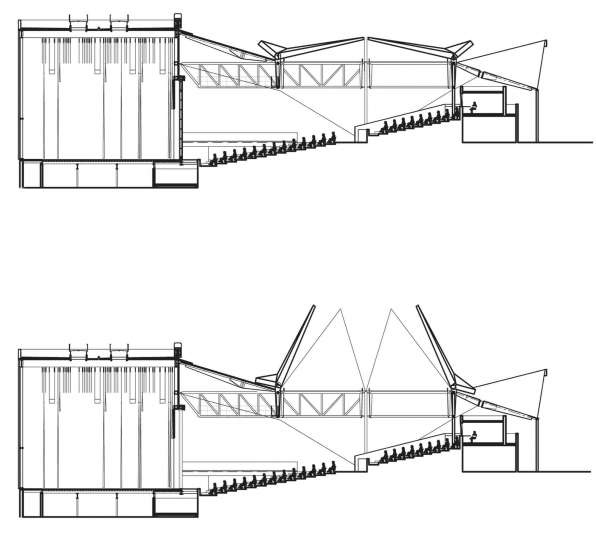
\includegraphics[width = 0.8\linewidth]{Figures/Bengt_theatre.jpg}
    \caption{Schematic Diagram of Bengt sjostrom starlight theatre, Image credit: www.archdaily.com}
    \label{fig:Bengt_theatre}
\end{figure} 

According to Maxwell's Lemma, the lightest (and therefore most efficient) structure separates compressive and tensile elements, this leads to a special class of Deployable structures called Tensegrity, Tensional integrity or Floating compression. Such structures consist of compression members floating in a net of tension members and the compression members do not usually touch each other. Since there is no bending, such structures are extremely efficient and have high rigidity-to-weight ratio. \cite{pellegr}

\section{Mechanisms and States of self stress}
Pin jointed frameworks can be classified into truss and mechanisms based on their connectivity. While a truss is defined as a rigid structure capable of carrying loads when simply supported, according to classical definition, Mechanism is defined as a system of rigid elements connected through pins and joints capable of movement. These mechanisms are classified into several groups such as planar mechanisms, spatial mechanisms, spherical mechanisms and so on. This classification can also be examined in terms of Static and Kinematic Indeterminacy.\cite{Pelle}


The assemblies in which all member forces can be determined using the equations of equilibrium are classified as statically determinate structure. Another equivalent definition of static determinacy is that for a given system, the number of equations is equal to the number of unknowns and the coefficient matrix is non-singular. Similarly Kinematic determinate structures are the assemblies in which the position of the nodes can be determined exactly (on one side of the base plane) based on the lengths of bars. kinematically indeterminate structures are the assemblies in which position of nodes can not be determined uniquely and they have one or more mode of inextensional deformation. It means that such an assembly can distort without change in member lengths which essentially makes it a mechanism. In a similar manner, state of self stress is related to statically indeterminate structures. When an assembly has states of self stress, it's member can have forces without application of any external load. 

Deployable structures generated using mechanisms belong to the structural class. While the Maxwell's rule provides condition for the static and kinematic determinacy based on the equality of number of equations and number of unknowns when structure is adequately connected to the foundation as 
\begin{equation}
    b = dJ,
\label{eq:cacona}
\end{equation}

\noindent where b is the total number of bars, d is dimension of the problem and J is the number of non foundation joints.

However, exceptions exist to this rule in form of structures which satisfy Maxwell's rule but still are kinematically indeterminate.

A more exhaustive treatment of equilibrium and kinematic matrix provides a more complete explanation for these anomalies.

The equilibrium matrix of a structure is a $(3j - k)$ by $b$ matrix which relates the member tensions $\boldsymbol{t}$ with external loads $\boldsymbol{f}$ as
\begin{equation}
    \boldsymbol{A.t = f}
    \label{eq:cacona}
\end{equation}
\noindent where j is total number of joints, k is number of kinematic constraint on foundation joints and b is the total number of bars.

In a similar manner, for small deformations, member elongations $\boldsymbol{e}$ and displacements of joints $\boldsymbol{d}$ can be related using a $b$ by $(3j - k)$ matrix $\boldsymbol{B}$ as
\begin{equation}
    \boldsymbol{B.d = e}
    \label{eq:cacona}
\end{equation}

\noindent Using the principle of virtual work, one can show that $\boldsymbol{B = A^T}$. The fundamental sub-spaces associated with these matrices and there significance are as following:

\begin{enumerate}
    \item \textit{Column Space of A} : Provides the range of $\boldsymbol{f}$ that can be supported by the structure and modes of displacement that require elongation of one or more bars.

    \item\textit{Left nullspace of A} : Describes the range of $\boldsymbol{f}$ that can not be supported by the structure in its original configuration and it is the space spanned by inextensional mechanisms.

    \item\textit{Row Space of A} : Spans the space generated by bar tensions in equilibrium with the applied load and describes geometrically compatible bar elongations.

    \item\textit{Nullspace of A} : represents sets of tension which are in equilibrium with zero loads (states of self stress) and bar elongations forbidden by the geometry.
\end{enumerate}



The analysis of these sub-spaces associated with the matrices $\boldsymbol{A}$ and $\boldsymbol{B}$ results in modified Maxwell's equation as
\begin{equation}
    s = b - r_{A},  \hspace{1cm} m = 3j - k - r_{A},
    \label{eq:cacona}
\end{equation}
\noindent subtracting two equations we get
\begin{equation}
    s - m = b - 3j + k
    \label{eq:cacona}
\end{equation}
\noindent here s is the number of states of self stress, and m is the number of mechanisms present in the structure. $r_{A}$ is the rank of the matrix A.

Further investigation of these matrices provides us with a way to distinguish between finite and infinitesimal mechanisms. These insights coupled with the interpretation of fundamental sub-spaces provide the information necessary for design of mechanism based deployable structures\cite{Pelle}.


\section{Origami}
Origami is a Japanese word derived from ori meaning "folding", and kami meaning "paper" and stands for the art of paper folding. Another term closely associated with Origami is Kirigami, unlike origami cutting of the paper is allowed in Kirigami. The Origami technique comprises of several basic basic folds like valley and mountain folds, pleats, reverse folds, squash folds, and sinks, which are used to generated complex patterns and shapes using a single sheet of paper.


The art of Origami has found several applications in the industries such as medical and space industry and continues to inspire new techniques in other fields. The techniques of origami are currently being investigated for development of new materials and tools such as Metamaterials, Sandwich panels, drones and robots.

Origami aids in the development of deployable structures through the generative pathway\cite{rivas2015deployable}. Origami provides a way to pack the structures into compact spaces. The origami models can be morphed into real structure by developing the equivalent bar and hinge models\cite{FilipBarandHinge}. The simplicity of such models make them well suited for the engineering community, and their efficiency make them suitable for design problems such as optimization and parameterization of geometric origami variations.The application of origami for development of deployable structures can be best illustrated by examples as shown in the Fig~\ref{fig:OrigamiEx}.
\begin{figure}[htbp]
    \centering
    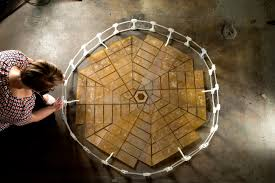
\includegraphics[width = 0.8\linewidth]{Figures/Origami_NASA.jpg}
    \caption{Origami based deployable solar panel for space application, Image credit: NASA}
    \label{fig:OrigamiEx}
\end{figure}


Furthermore the concepts of origami combined with the metamaterials provide a way for the structures which follow different energy pathways during deployment and contraction, which makes them highly desirable since they can be designed to resist immediate collapse by providing an energy barrier in their contraction pathway\cite{Zha}. This also adds to the reliability for use of deployable structures making their stability less dependent on locking mechanisms. In addition to this Origami can also be used for programming curvatures\cite{Dud}, and development of metamaterials\cite{Filip}.

In simple cases of pure origami based deployable hollow triangulated cylinders, based on the energy required the structures can be classified as easy-deploy-easy-collapse (requiring no or minimal energy for deployment as well as collapse) or hard-deploy-hard-collapse (requiring significant amount of energy for deployment as well as collapse). Easy-deploy-easy-collapse structures generate minimal strain in members of their equivalent bar and hinge model while hard-deploy-hard-collapse structure create large strains leading to even failure in case of conventional materials\cite{Zha,FilipBarandHinge}. The tubes can be designed to fall in one of the types by varying simple parameters which is shown in the next chapter.

\section{Mechanical Metamaterials}
Metamaterials are defined as the materials which are engineered for the properties that are not present in naturally occurring materials. Metamterials gain their property from their internal structure and connectivity rather than the materials properties. Based on the property with which a metamaterial is concerned, it is classified into one of the several sub-divisions such as Electromagnetic Metamaterials, Thermo-Electric Metamaterials and so on. Mechanical metamaterials are concerned with mechanical properties of matter and focuses on achieving unusual values for mechanical parameters such as density, Poisson's ratio, and compressibility. Recent development in the field are associated with the development of exotic functionalities such as pattern and shape transformation in response to mechanical forces, unidirectional guiding of motion and waves and reprogrammable stiffness\cite{Berto, Surj}.

The domain of metamaterials which deals with materials having tunable stiffness forms a connection between metamaterials and deployable structure. Simplest instance of use of metamaterials in deployables is in the structures which have different energy paths for deployment and collapse, as explained earlier. Using a conventional material, if an element experiences compression during the process of deployment, it will experience tension while collapsing and usually the stiffness in tension as well as compression is same for materials and thus energy path followed is same for two deployment as well as collapse, however for material which exhibit different stiffness for tension and compression will have different profiles for two process and can lead to structures which deploy easily but offer resistance for collapsing and vice versa.\cite{Zha} 

Furthermore soft metamaterials and materials at the verge of instability have parameters which can be tuned to develop hinges and joints as part of elements engendering the possibility of a unified deployable systems without any external joints.\cite{Baardink489, Rock}

Design of metamaterials also draws from Origami, Mechanism, Topology, and form finding making a cohesive whole of all these ideas\cite{Filip, Rock}.

\section{Form Finding}
The primary motive of the form-finding process is to identify the geometry that sustains the load coming on the structure most efficiently or the shape a structure takes under a given load. In cases when elasticity and geometric constraints are intertwined, for example structure such as elastic gridshells which buckle by design, actuated shapes are difficult to predict using classical methods. Such cases suggest the presence of multi-stable states and the analysis requires inclusion of higher modes of the structure. Such techniques can applied in the opposite direction as well to determine the boundary conditions and forces that need to be applied on the structure to achieve the desired shape.\cite{Baek75} 

The ideas of form finding are usually applied in the reverse direction to determine the boundary conditions which will lead to the structure taking the desired shape. The deformations involved are usually large and material needs to be elastic during the entire process so that the structure can be deployed and collapsed a number of times, this provides another entry point for the application of metamaterials.

An example where this relationship is elicited is that of form finding in elastic gridshells. Initially planar elastic grid is actuated into a shell like structure by loading their extremities. It was observed that the resulting shapes are complex even for simple configuration and indicated the presence of multi-stable states and higher order modes in the actuated grid. However it is possible to parameterize these complex shape and by varying these parameters desired actuated shape can be obtained\cite{Baek75}.

\section{Elastic Bilayers}
Elastic Bilayers stands for shape shifting thin sheets made up of active materials that respond to stimuli such as heat, light and humidity. Such layers are designed by solving the geometric inverse problem of determining the growth factors and directions for a given isotropic elastic bilayer to grow into a target shape by posing and solving an elastic energy minimization problem. Such techniques aid in engineering complex functional shapes in tissues, and actuation systems in soft robotics.\cite{va}

In general nonuniform in-plane growth of thin sheets results in out of plane buckling. This process is responsible for several process in nature such as shaping of leaf and blooming of flowers. Generally, such sheets settle in residually strained configuration which is a local minima of the energetic cost of stretching and bending the sheet. Since it's a local minima, this state might not be unique. By solving the inverse problem one can design the layer such that it can be used to achieve any target surface shape from any reference shape\cite{va}. Similar to the case of form finding, this involves parameterizing the surface and solving the inverse problem.

\section{Topological Mechanics}
In Mathematics, Topology is defined as the study of properties of a geometric object that are preserved under continuous deformations, such as stretching, twisting, crumpling and bending. The concepts from Topology are aiding the development of novel materials such as topological insulators, and topological photonics. In the recent times, the concepts from electronic topological states are being applied to mechanics to identify topological mechanical properties. Topological mechanics encompasses the study of topological phonon modes of the material, which has applications in development of mechanical insulators and metamaterials with topologically protected mechanical properties.\cite{Ma, Rock, Baardink489, Che}

Topology involves the study of connectivity of different elements in a system and is essential to the idea of deployable structures. Topology plays an important role in determining the member connectivity in deployable trusses and folding motions of Origami and Kirigami\cite{Che}.

In addition to the deployable structures, It has a huge role in development of metamaterial\cite{Rock, Berto, Surj} and lattice mechanics\cite{Ma}. Topology can be used to control the mechanical properties of a material along an edge or around a localized defect, topological polarization of a network governs along with its variation and orientation define the rigidity of the network. The topology of the lattices can be varied to move between states with dramatically varying mechanical properties such as elastic modulus, wave characteristics and so on. 

\section{Lattices \& Non-Affine Deformations}
Lattice is an ordered arrangement of particles which repeats infinitely in all dimensions of the lattice. The unit cell of a lattice is defined as the smallest repeating unit having the full symmetry of the lattice and Structure of a lattice is described by its unit cell. A lattice may have more than one unit cell which when translated can generate entire lattice. A special class of lattices are termed as Maxwell lattices. Maxwell lattices are mechanical frames having average coordination number equal to twice their spatial dimension, this leaves them on verge of mechanical instability. Fourier Transform of these lattices also results in lattices, which are called Reciprocal Lattices and present the lattice in reciprocal space. Reciprocal Lattices are used for determining the phonon modes which helps in design of materials with topologically protected material properties.


Changes in the metric properties of a continuous body is defined as deformation, this indicates that a curve drawn on original body will change its length after the body is deformed. Usually deformations are affine which means that the deformations can be described in terms of affine transformation, or equivalently local strain in a sample after deformation is identical everywhere and equal to the macroscopic strain. All deformations other than affine deformations are termed as non-affine deformation. One of the principal sources of non-affinity is a space or time dependent elastic constant. The local environment in a disordered solid varies in space, depending crucially on local connectivity or coordination such that the local displacement $\textbf{u}$ may not be simply related to the applied stress $\boldsymbol{\sigma}$. Such non-affine displacements are present even at zero temperature, are material dependent, and vanish only for homogeneous crystalline media without defects\cite{Gang}.

The deployable structure connects with the lattices at two level, on a trivial level, the lattices can be considered as a special kind of structure and mechanisms involved in such structures connect them directly with the ideas of deployable structure. Lattices require special attention owing to their periodic boundary conditions. Depending on the topology of lattice, actuation may propagate throughout the lattice or may cease within a few unit cells \cite{Neli}. Furthermore, it can be shown that static determinacy and kinematic determinacy can not exist in these structures concurrently \cite{Gues}. 

On a more elaborate level, Metamaterials connect the deployable structures with lattices since design of metamaterials requires realization and application of lattice mechanics and properties which is ultimately utilized for development of deployable structures. Lattice mechanics is essential to the development of metamaterials with unusual elastic modulus and phonon gaps.\cite{Ma}


\chapter{ Origami Models: Simulations and Findings}

%Check for mail with subject "Energy diagrams for hexagonal cell"

\section{Deployable Origami Tubes}
Two types of triangulated Origami tubes were developed and were tested for deployability. In accordance with the idea of energy profile based on the sum of two angles of the triangular units of the tubes easy-deploy-easy-collapse and hard-deploy-hard-collapse tubes were developed\cite{Zha}. 

The cylindrical tube is generated by joining two edges of the sheet show in the Fig~\ref{fig:AlphaBeta}. For the angles shown in Fig~\ref{fig:AlphaBeta}, if $\alpha + \beta < 90^{\circ}$ the tube is of the easy-deploy-easy-collapse (Fig~\ref{fig:EDEC}) type and if the sum is greater than $90^{\circ}$ i.e $\alpha + \beta > 90^{\circ}$ the mechanism is of hard-deploy-hard-collapse type(Fig~\ref{fig:HDHC}). It was observed from analysis of numerical model that for the hard-deploy-hard-collapse model ($\alpha = 50^{\circ}, \beta = 50^{\circ}$), the strain in equivalent bar hinge model would be of the order 20\% and hence the collapse is not possible in normal paper model. Also the hard-deploy-hard-collapse model carried significant lode before the paper model underwent local buckling at its creases.
\begin{figure}[htbp]
\centering
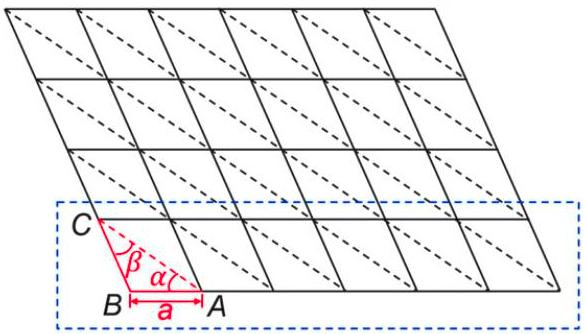
\includegraphics[width=0.6\linewidth]{Figures/AlphaBeta.jpg}
\caption{Crease Pattern For Cylindrical Tube}
\label{fig:AlphaBeta}
\end{figure}

\begin{figure}
\centering
\begin{minipage}{.5\textwidth}
  \centering
  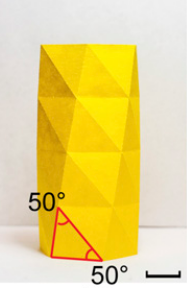
\includegraphics[width=.4\linewidth]{Figures/HardDeploy.png}
  \captionof{figure}{Hard-Deploy-Hard-Collapse}
  \label{fig:EDEC}
\end{minipage}%
\begin{minipage}{.5\textwidth}
  \centering
  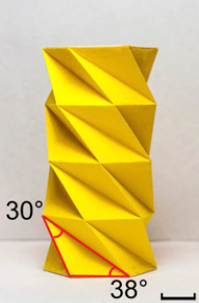
\includegraphics[width=.4\linewidth]{Figures/EasyDeploy.png}
  \captionof{figure}{Easy-Deploy-Easy-Collapse}
  \label{fig:HDHC}
\end{minipage}
\end{figure}


\section{Energy Profiles}
The simulated energy profiles for the origami tubes are shown in the Fig~\ref{fig:EnergyProfile}. The simulation was performed for the equivalent bar hinge model.
\begin{figure}[htbp]
\centering
	\subfigure[Easy-Collapse-Easy-deploy energy profile ]{
	\centering
		\label{fig:ECEDEP}
        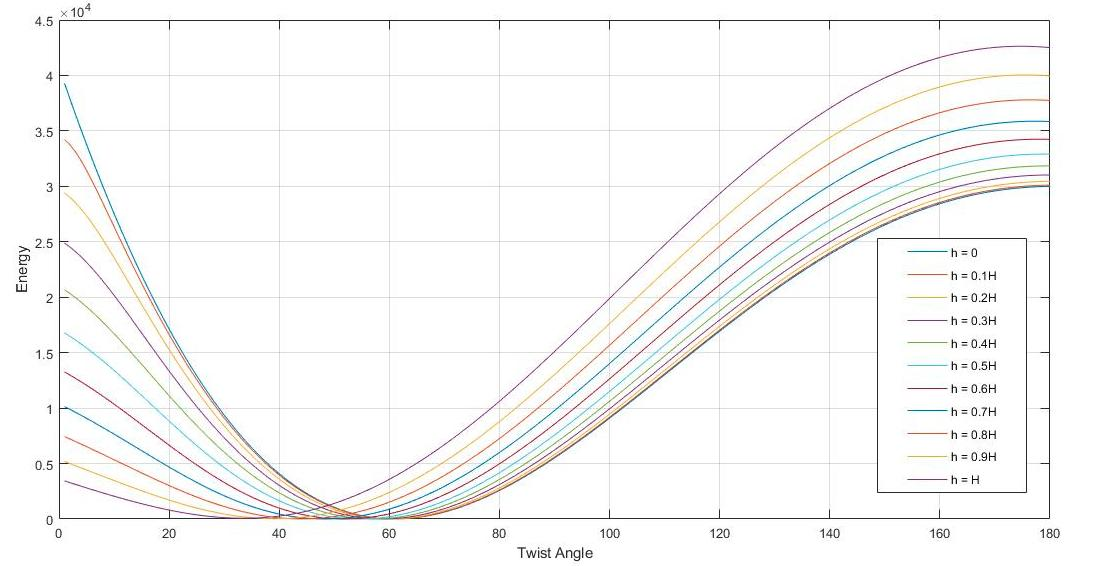
\includegraphics[width=1\linewidth]{Figures/EDEC.jpg}}
	\subfigure[Hard-Collapse-Hard-deploy energy profile]{
	\centering
		\label{fig:HCHDEP}
		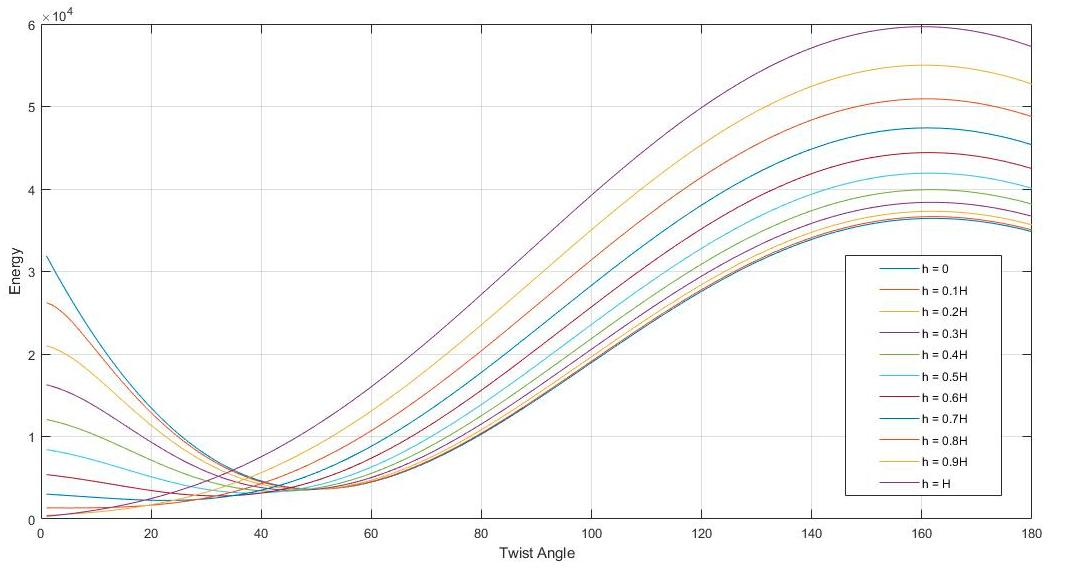
\includegraphics[width=1\linewidth]{Figures/HDHC.jpg}}
	\caption{Energy Profiles}
	\label{fig:EnergyProfile}
\end{figure}

As it can be seen from the energy profile obtained by computing energy in the structure at various stages of deployment, the easy-deploy-easy-collapse structure presents negligible energy barrier as opposed to the hard-deploy-hard-collapse structure in which significant energy barrier is present for process of deployment as well as collapse. 

Using metamaterials, a structure which presents no energy barrier during deployment but exhibits resistance to collapse can be developed. This will provide the reliability to the deployable structure without being dependent on locking mechanisms for its stability.

\section{Physical Models}
Physical models of the lattice were also developed to qualitatively validate the energy profiles obtained from simulation. The folding patterns used for the models are shown in the Fig~\ref{fig:HCHD_fold} and Fig~\ref{fig:ECED_fold}.
\begin{figure}[htbp]
    \centering
    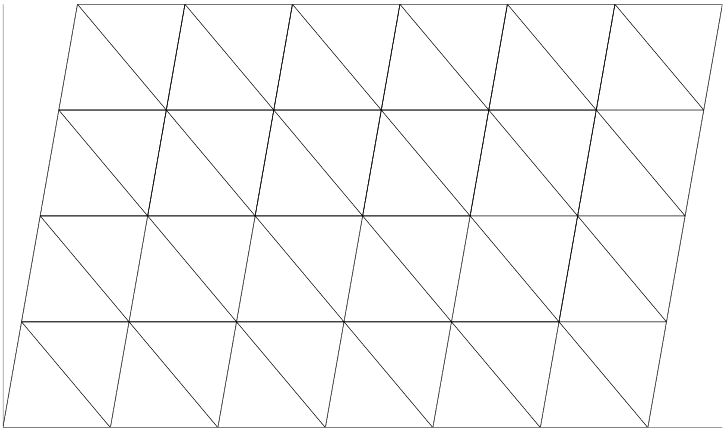
\includegraphics[width = 0.5\linewidth]{Figures/50_50_180_fold.png}
    \caption{Folding pattern for Hard-Collapse-Hard-Deploy Origami tube}
    \label{fig:HCHD_fold}
\end{figure}
\begin{figure}[htbp]
    \centering
    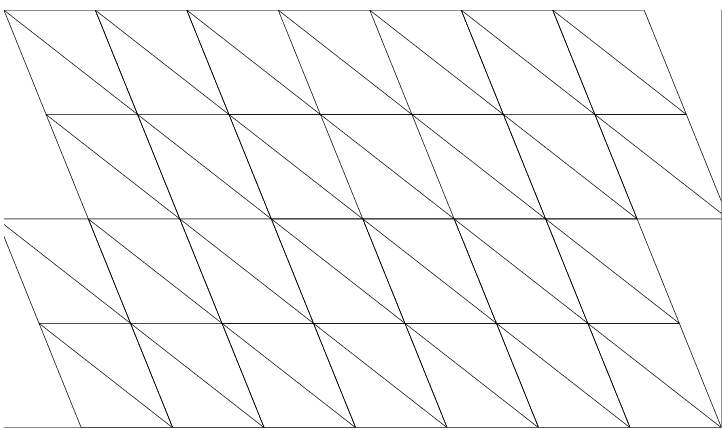
\includegraphics[width = 0.5\linewidth]{Figures/38_30_112_fold.png}
    \caption{Folding pattern for Easy-Collapse-Easy-Deploy Origami tube}
    \label{fig:ECED_fold}
\end{figure}

The models developed using these folding patterns are shown in the figures below. As predicted using the energy profiles, Easy-Deploy-Easy-Collapse type origami tube easily collapse under very small load from state shown in Fig~\ref{fig:EDEC_model} to the state shown in Fig~\ref{fig:EDEC_Model_Collapsed}. Also, the Hard-Deploy-Hard-Collapse (Fig~\ref{fig:HDHC_model}) type tube did not collapse in a way similar to Easy-Deploy-Easy-Collapse type tube even under high load (Fig~\ref{fig:HDHC_Model_Loaded}), but as stated earlier, due to developing high strains the paper began to tear and tube buckled.

\section{Conclusion}
From the models and simulation of origami tubes stated above we can conclude that modelling these origami tubes using bar hinge models and using metamaterials with different strengths in elongation and compression we can modify the energy profiles during deployment and collapse such that we have an selective Easy-Deploy-Hard-Collapse or Hard-Deploy-Easy-Collapse type structure.

\begin{figure}[htbp]
\centering
\begin{minipage}{.4\textwidth}
  \centering
  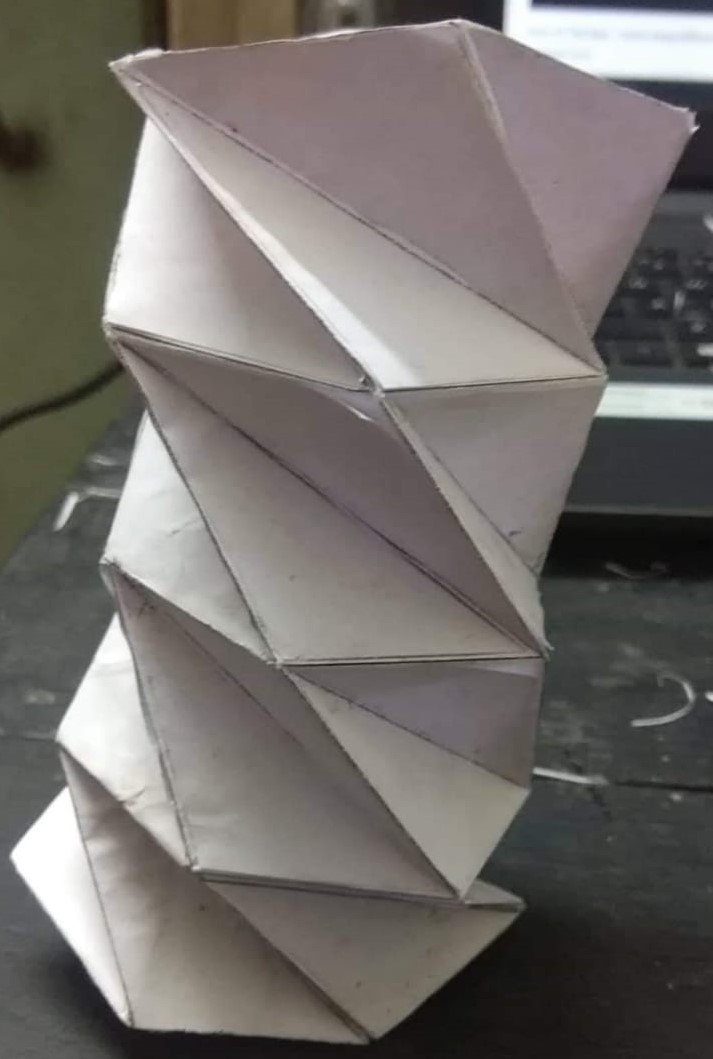
\includegraphics[width=.4\linewidth]{Figures/EDEC_Model.jpeg}
  \captionof{figure}{Easy-Deploy-Easy-Collapse physical model}
  \label{fig:EDEC_model}
\end{minipage}%
\hspace{2cm}
\begin{minipage}{.4\textwidth}
  \centering
  \vspace{2cm}
  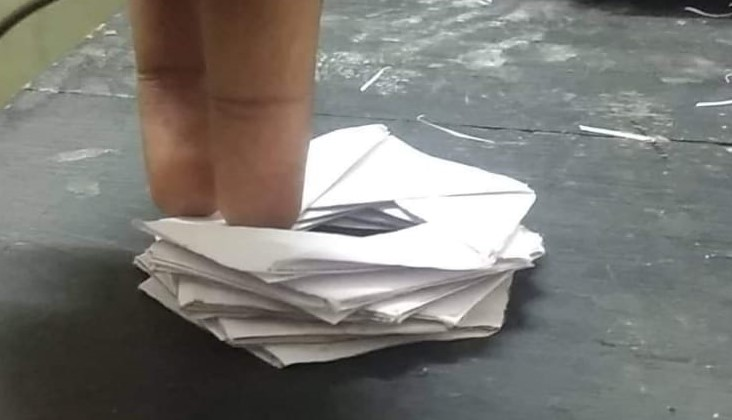
\includegraphics[width=.4\linewidth]{Figures/EDEC_Model_collapsed.jpeg}
  \captionof{figure}{Collapsed state of Easy-Deploy-Easy-Collapse Model}
  \label{fig:EDEC_Model_Collapsed}
\end{minipage}
\end{figure}
\vspace{-3cm}

\begin{figure}[htbp]
\centering
\begin{minipage}{.4\textwidth}
  \centering
  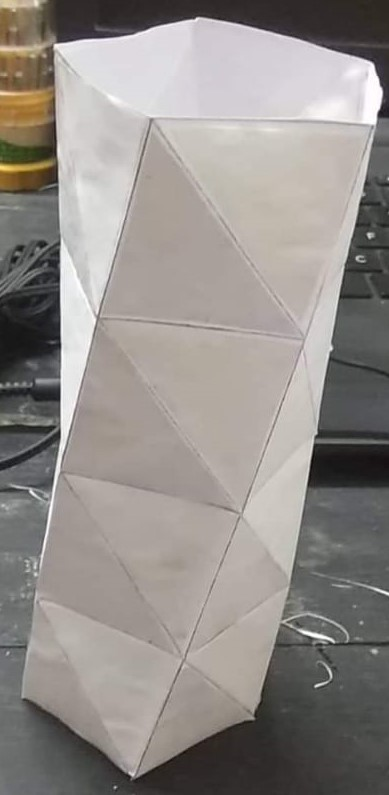
\includegraphics[width=.4\linewidth]{Figures/HDHC_Model.jpeg}
  \captionof{figure}{Hard-Deploy-Hard-Collapse physical model}
  \label{fig:HDHC_model}
\end{minipage}%
\hspace{2cm}
\begin{minipage}{.4\textwidth}
  \centering
  \vspace{0.4cm}
  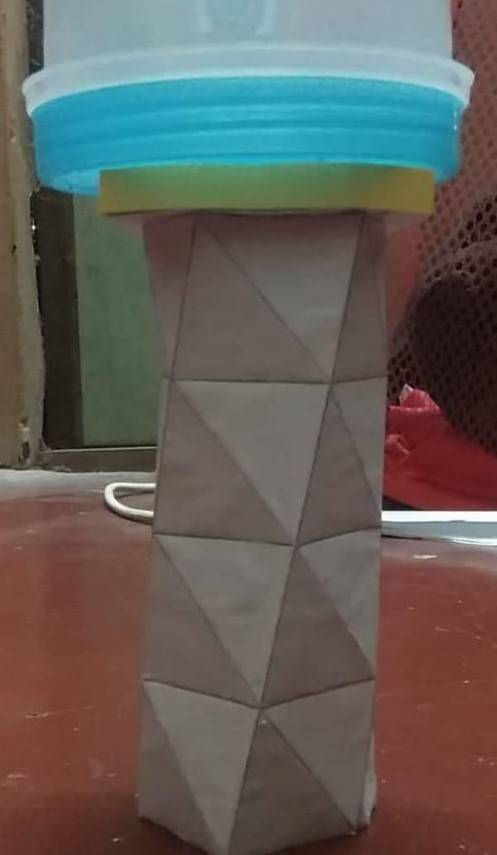
\includegraphics[width=.4\linewidth]{Figures/HDHC_Model_loaded.jpeg}
  \captionof{figure}{Hard-Deploy-Hard-Collapse Model under loading}
  \label{fig:HDHC_Model_Loaded}
\end{minipage}
\end{figure}
\chapter{Plate Models: Simulations and Findings}

The program models plates as spring ball systems with linear springs and is developed in Python 3.6. It employs an energy minimization based approach to determine the displacements of the plate at which balls are located. These displacements can be interpolated to estimate the displacements of any point on the plate.

The program primarily generated rectangular model and can generate several kind of models such as plane single layer rectangular lattice with all possible combinations of in-plane diagonals (Fig~\ref{fig:plane_rectangular}, Fig~\ref{fig:Plane_rect_with_bracing1}, and Fig~\ref{fig:Plane_rect_with_bracing2}), and cuboidal lattices with all kinds of diagonals possible (Fig~\ref{fig:3D_rect1}, Fig~\ref{fig:3d_rect2}, and Fig~\ref{fig:3d_rect3}). In addition the support conditions in X-, Y- and Z- direction can be specified at any of the nodes independently, as shown in the figures with triangular symbols.


\begin{figure}[htbp]
\begin{minipage}{0.3\textwidth}
    \centering
    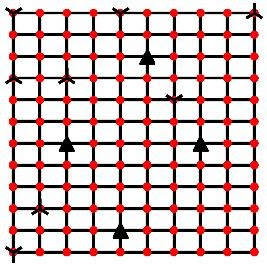
\includegraphics[width = 1\textwidth]{Figures/10x12simple_plane.jpg}
    \caption{Plane rectangular lattice}
    \label{fig:plane_rectangular}
\end{minipage}
\hspace{5mm}
\begin{minipage}{0.3\textwidth}
    \centering
    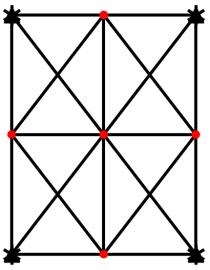
\includegraphics[width = 1\textwidth]{Figures/3x3braced_plane.jpg}
    \caption{Plane rectangular lattice with both bracing}
    \label{fig:Plane_rect_with_bracing1}
\end{minipage}
\hspace{5mm}
\begin{minipage}{0.3\textwidth}
    \centering
    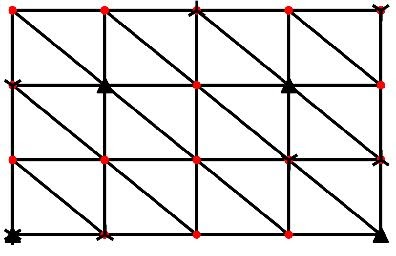
\includegraphics[width = 1\textwidth]{Figures/5x4_braced_plane.jpg}
    \caption{Plane rectangular lattice with one bracing}
    \label{fig:Plane_rect_with_bracing2}
\end{minipage}
\end{figure}

\begin{figure}[!htbp]
\begin{minipage}{0.3\textwidth}
    \centering
    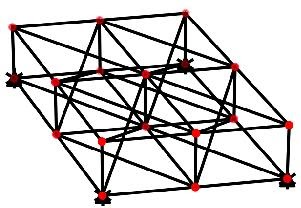
\includegraphics[width = 1\textwidth]{Figures/3x3reduced_bracings3d.jpg}
    \caption{3D rectangular lattice with few braces}
    \label{fig:3D_rect1}
\end{minipage}
\hspace{5mm}
\begin{minipage}{0.3\textwidth}
    \centering
    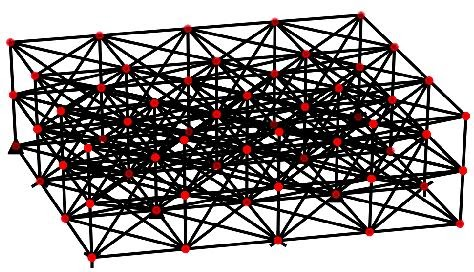
\includegraphics[width = 1\textwidth]{Figures/5x43d3layer.jpg}
    \caption{3D rectangular 3-layer lattice with braces}
    \label{fig:3d_rect2}
\end{minipage}
\hspace{5mm}
\begin{minipage}{0.3\textwidth}
    \centering
    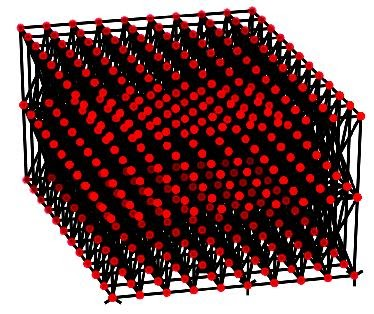
\includegraphics[width = 1\textwidth]{Figures/10x12braced3d3layer.jpg}
    \caption{3D rectangualar 3-layer lattice with all possible braces}
    \label{fig:3d_rect3}
\end{minipage}
\end{figure}

\section{Model Details}
The model works on energy minimization principles and can simulate all kind of strain fields and loading. The model uses L-BFGS-B optimization algorithm from scipy.optimize toolbox of Python. Broyden–Fletcher–Goldfarb–Shanno (BFGS) algorithm is an iterative method for solving unconstrained nonlinear optimization problems. L-BFGS-B is Limited memory-BFGS algorithm extended to handle simple box constraints (support conditions in our case). 

Design variables are the coordinates of the nodes stacked together. These variable determine the length of the springs in any given state which in turn determines the energy of the system.

Energy of the system is defined as:
\begin{equation}
    E = \sum_{i = 1}^{N}\frac{1}{2}k_i (l_i - l_{0i})^2 - \boldsymbol{f.\Delta r}
\end{equation}
where:\\
\\
    $E$: Total energy of the system\\
    $N$: total number of springs\\
    $K_i$: Stiffness of the $i^{th}$ spring\\
    $l_i$: current length of $i^{th}$ spring\\
    $l_{0i}$: Natural length of $i^{th}$ spring\\
    $\boldsymbol{f}$: Load vector\\
    $\Delta r$: Displacement vector\\
    
The optimization program also uses the derivatives, which are given as:
\begin{equation}
    \frac{\partial E}{\partial x_i} = \sum_{j \in T_i} k_j(x_j - x_{0j})(1 - \frac{l_{0j}}{\sqrt{(x_j - x_{0j})^2 + (y_j - y_{0j})^2 + (z_j - z_{0j})^2}}) - f_{x_i}
\end{equation}
\begin{equation}
    \frac{\partial E}{\partial y_i} = \sum_{j \in T_i} k_j(y_j - y_{0j})(1 - \frac{l_{0j}}{\sqrt{(x_j - x_{0j})^2 + (y_j - y_{0j})^2 + (z_j - z_{0j})^2}}) - f_{y_i}
\end{equation}
\begin{equation}
    \frac{\partial E}{\partial z_i} = \sum_{j \in T_i} k_j(z_j - z_{0j})(1 - \frac{l_{0j}}{\sqrt{(x_j - x_{0j})^2 + (y_j - y_{0j})^2 + (z_j - z_{0j})^2}}) - f_{z_i}
\end{equation}

where\\
$T_i$: set of all springs connected to node $i$\\
$f_{x_i}$, $f_{y_i}$, and $f_{z_i}$: force at node $i$ in $X-$, $Y-$, and $Z-$ directions respectively

\section{Theory}
The models are validated for point load at centre using Classical Plate Theory (CPT), also known as Kirchhoff-Love theory and First-order Shear deformation Theory (FSDT), also known as Mindlin–Reissner plate theory. A point load applied at the centre of the plate is used for the calibration and validation. More details about the models are in their respective sections.

\subsection{Classical Plate Theory}
According to classical plate theory, displacement field is based on the following assumptions, called Kirchhoff hypothesis
\begin{enumerate}
    \item Straight line perpendicular to the mid-surface (i.e., transverse normals) before deformation remain straight after deformation.
    \item The transverse normals do not experience elongation (i.e., they are in inextensible).
    \item The transverse normals rotate such that they remain perpendicular to middle surface after deformation.
\end{enumerate}

Following these assumptions, the strains are found to be as given in eq~\ref{eq:CPT_strain1} - eq~\ref{eq:CPT_strains_last}.

\begin{equation}
    \epsilon_{xx} = \frac{\partial u_0}{\partial x} + \frac{1}{2}(\frac{\partial w_0}{\partial x})^2 - z\frac{\partial^2 w_0}{\partial x^2}
    \label{eq:CPT_strain1}
\end{equation}
\begin{equation}
    \epsilon_{yy} = \frac{\partial v_0}{\partial y} + \frac{1}{2}(\frac{\partial w_0}{\partial y})^2 - z\frac{\partial^2 w_0}{\partial y^2}
\end{equation}
\begin{equation}
    \epsilon_{zz} = \frac{1}{2}(\frac{\partial u_0}{\partial y} + \frac{\partial v_0}{\partial x} + \frac{\partial w_0}{\partial x}\frac{\partial w_0}{\partial y} - 2z\frac{\partial^2 w_0}{\partial x\partial y})
\end{equation}
\begin{equation}
    \epsilon_{xz} = \epsilon_{yz} = \epsilon_{zz} = 0
    \label{eq:CPT_strains_last}
\end{equation}

Using the principle of virtual displacement and strains defined above, the governing equation for CPT is obtained as eq~\ref{eq:gov_eqn} for a homogenous isotropic plate.

\begin{equation}
    \label{eq:gov_eqn}
    D\nabla^2\nabla^2 w_0 + kw_0 = q - \frac{1}{ 1 - \nu}\nabla^2 M_T
\end{equation}
where\\
\begin{equation}
    D = \frac{Eh^3}{12(1 - \nu^2)}
    \label{eq:D}
\end{equation}

using Navier's solution for a point load of magnitude $Q_0$ applied at the centre of a square plate of dimension $a$, the analytical equation obtained for transverse displacement at centre using first ten element of the series is:
\begin{equation}
    w_0(x_c, y_c) = 0.0116\frac{Q_0a^2}{D}
    \label{eq:w_CPT}
\end{equation}

Eq~\ref{eq:w_CPT} will be used to calibrate and validate the model as shown later.

\subsection{First-order Shear Deformation Theory}
The first-order shear deformation theory is arrived at by relaxing the third assumption of the Kirchhoff-Love plate theory, which states that transverse normal remain perpendicular to middle surface after deformation, by allowing for an arbitrary constant rotation of transverse normals. The assumption that transverse normals remain straight after deformation holds for first order theory by can be dismissed by using higher order theories.

using the modified assumptions, the strains are as following:

\begin{equation}
    \epsilon_{xx} = \frac{\partial u_0}{\partial x} + \frac{1}{2}(\frac{\partial w_0}{\partial x})^2 + z\frac{\partial\phi_x}{\partial x}
    \label{eq:FSDT_strain1}
\end{equation}
\begin{equation}
    \epsilon_{yy} = \frac{\partial v_0}{\partial y} + \frac{1}{2}(\frac{\partial w_0}{\partial y})^2 + z\frac{\partial\phi_y}{\partial y}
\end{equation}
\begin{equation}
    \epsilon_{zz} = 0
    \label{eq:strain_z_FSDT}
\end{equation}
\begin{equation}
    \gamma_{xy} = (\frac{\partial u_0}{\partial y} + \frac{\partial v_0}{\partial x} + \frac{\partial w_0}{\partial x}\frac{\partial w_0}{\partial y}) - z(\frac{\partial\phi_x}{\partial y} + \frac{\partial\phi_y}{\partial x})
\end{equation}
\begin{equation}
    \gamma_{xz} = \frac{\partial w_0}{\partial x} + \phi_x
\end{equation}
\begin{equation}
    \gamma_{yz} = \frac{\partial w_0}{\partial y} + \phi_y
    \label{eq:FSDT_last}
\end{equation}

Using the strains from eq~\ref{eq:FSDT_strain1} - eq~\ref{eq:FSDT_last}, for small deflection and rotation, we get governing equation for bending as,

\begin{equation}
    K_sGh(\Delta^2w_0 + \frac{\partial\phi_x}{\partial x} + \frac{\partial\phi_y}{\partial y}) + q(x, y) = 0
    \label{eq:gov_eq_FSDT1}
\end{equation}
\begin{equation}
    D(\frac{\partial^2\phi_x}{\partial x^2} + \nu\frac{\partial^2\phi_y}{\partial x\partial y}) + \frac{D(1 - \nu)}{2}(\frac{\partial^2\phi_x}{\partial y^2} + \frac{\partial^2\phi_y}{\partial x\partial y}) - K_sGh(\frac{\partial w_0}{\partial x} + \phi_x) = 0
\end{equation}
\begin{equation}
    \frac{Gh^3}{12}(\frac{\partial^2\phi_x}{\partial x\partial y} + \frac{\partial^2\phi_y}{\partial x^2}) + D(\nu\frac{\partial^2\phi_x}{\partial x\partial y} + \frac{\partial^2\phi_y}{\partial y^2}) - K_sGh(\frac{\partial w_0}{\partial y} + \phi_y) = 0
    \label{eq:gov_eq_FSDT3}
\end{equation}

The solution to the eq~\ref{eq:gov_eq_FSDT1} - eq~\ref{eq:gov_eq_FSDT3} is obtained for the case of point load applied at the centre is obtained using Navier Solution. 

\section{Models and Results}
To validate the Python program and models developed, deflections resulting from a point load applied at the centre are checked with respect to analytical solutions available from theories described above. Following the comparison, possible reason for deviations, limitations and advantages are discussed.

The study is carried out with three kinds of model. Further, each model has three variant with varying number number of nodes and springs. Two types of studies are carried out for each variant, namely Constant Stiffness studies in which springs have constant stiffness irrespective of its length, and Constant Axial rigidity studies in which $EA$ is held constant for springs and their stiffness$(= EA/l)$ is inversely proportional to their lengths. Also to ensure that $\epsilon_{zz}$ is zero or at least close to zero (eq~\ref{eq:strain_z_FSDT} and eq~\ref{eq:CPT_strains_last}) the vertical spring are provided with stiffness orders of magnitude higher than in plane spring stiffness. Details of each of them can be found in their respective sections.

\subsection{Model 1}
The model 1 is composed of of a 3-layer simple cubic lattice type model. Dimension of the plate is 1~m x 1~m x 0.02~m. Stiffness of the springs in model are calibrated for displacement at centre for a 2 kN point load applied at centre with displacements at centre of an equivalent plate with $E = 2$ GPa and $\nu = 0.25$).

\subsubsection{Model 1 - Type A}
These models are type 1 model with 4 x 4 x 2 structure of cuboids of dimension 0.25~m x 0.25~m x 0.01~m stacked together as shown in the fig~\ref{fig:M1_a_XY} - fig~\ref{fig:M1_a_3D}.

\begin{figure}[!htbp]
\begin{minipage}{0.3\textwidth}
    \centering
    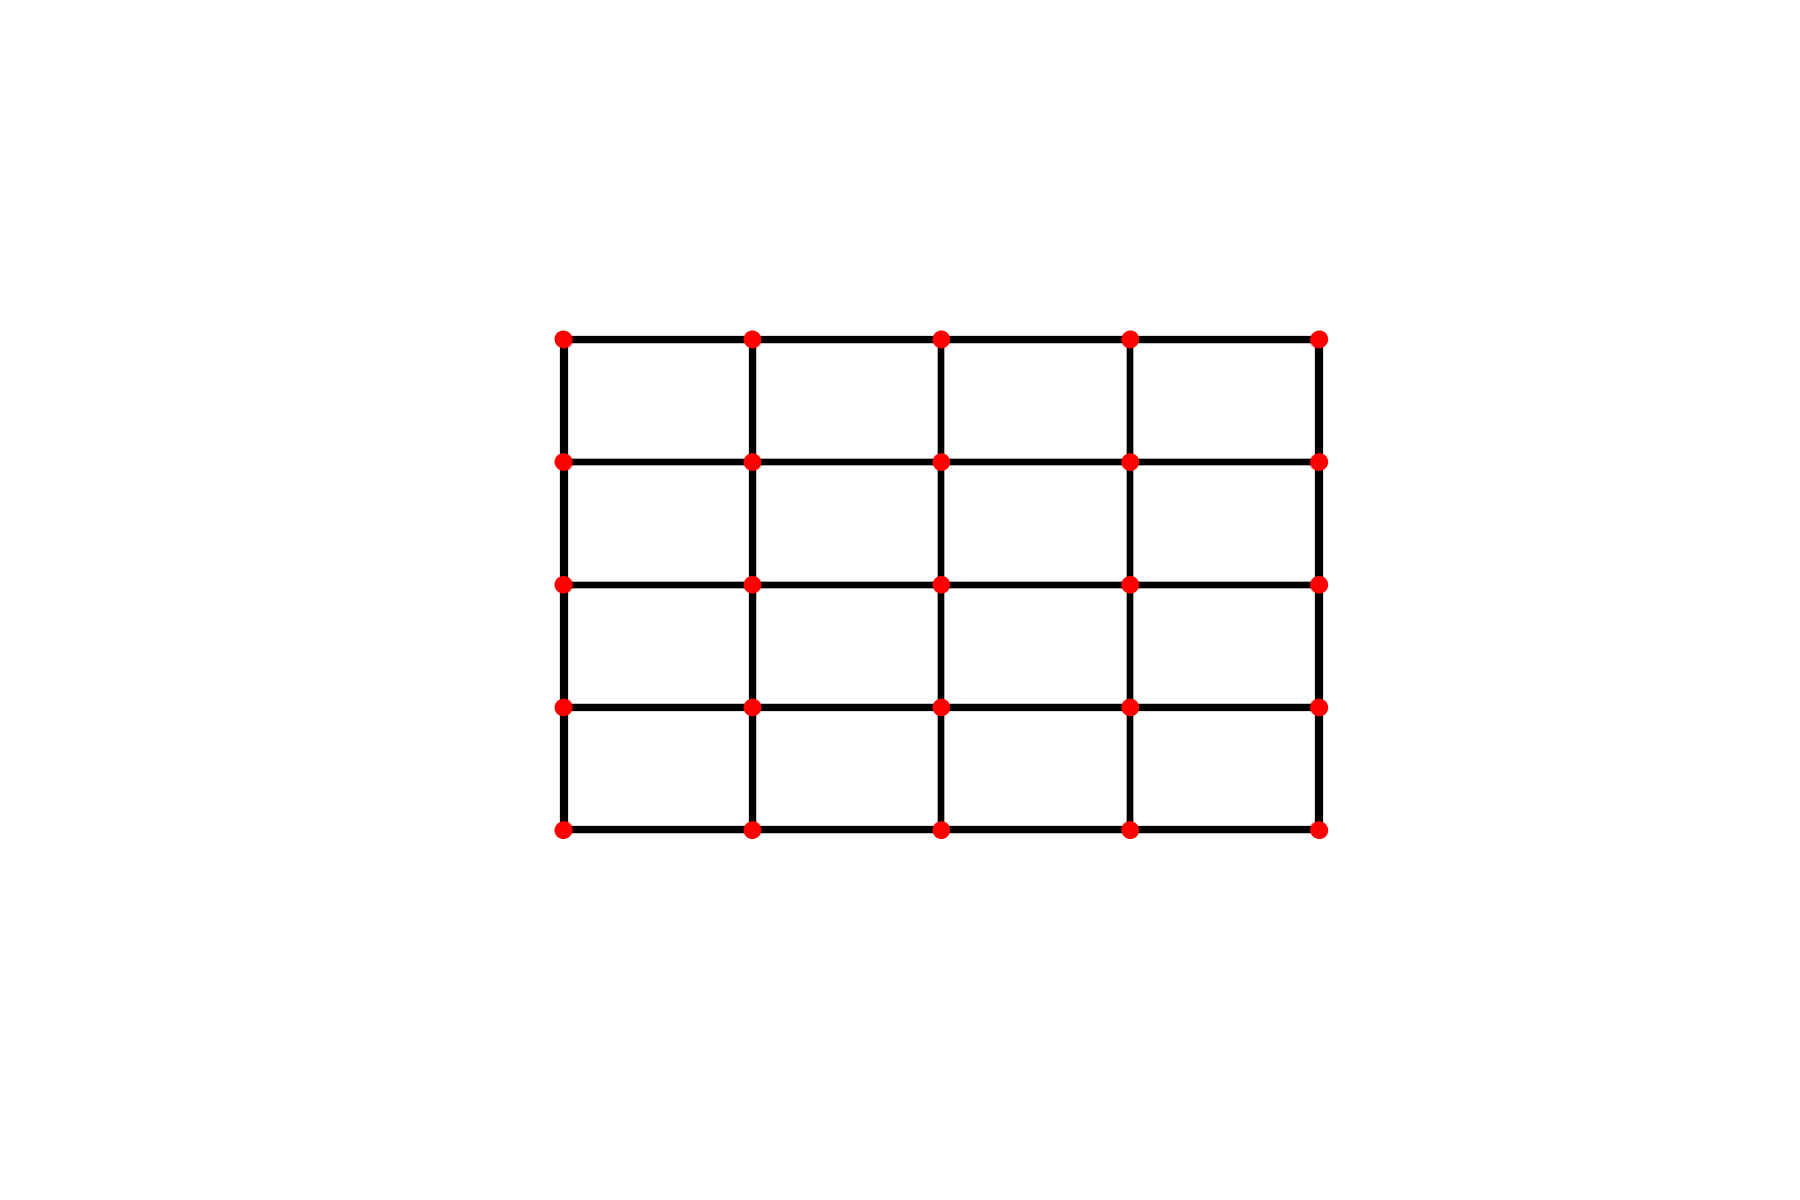
\includegraphics[width = 1\textwidth]{Figures/M1_type_a_XY.png}
    \caption{Model 1 - Type A - XY Projection}
    \label{fig:M1_a_XY}
\end{minipage}
\hspace{5mm}
\begin{minipage}{0.3\textwidth}
    \centering
    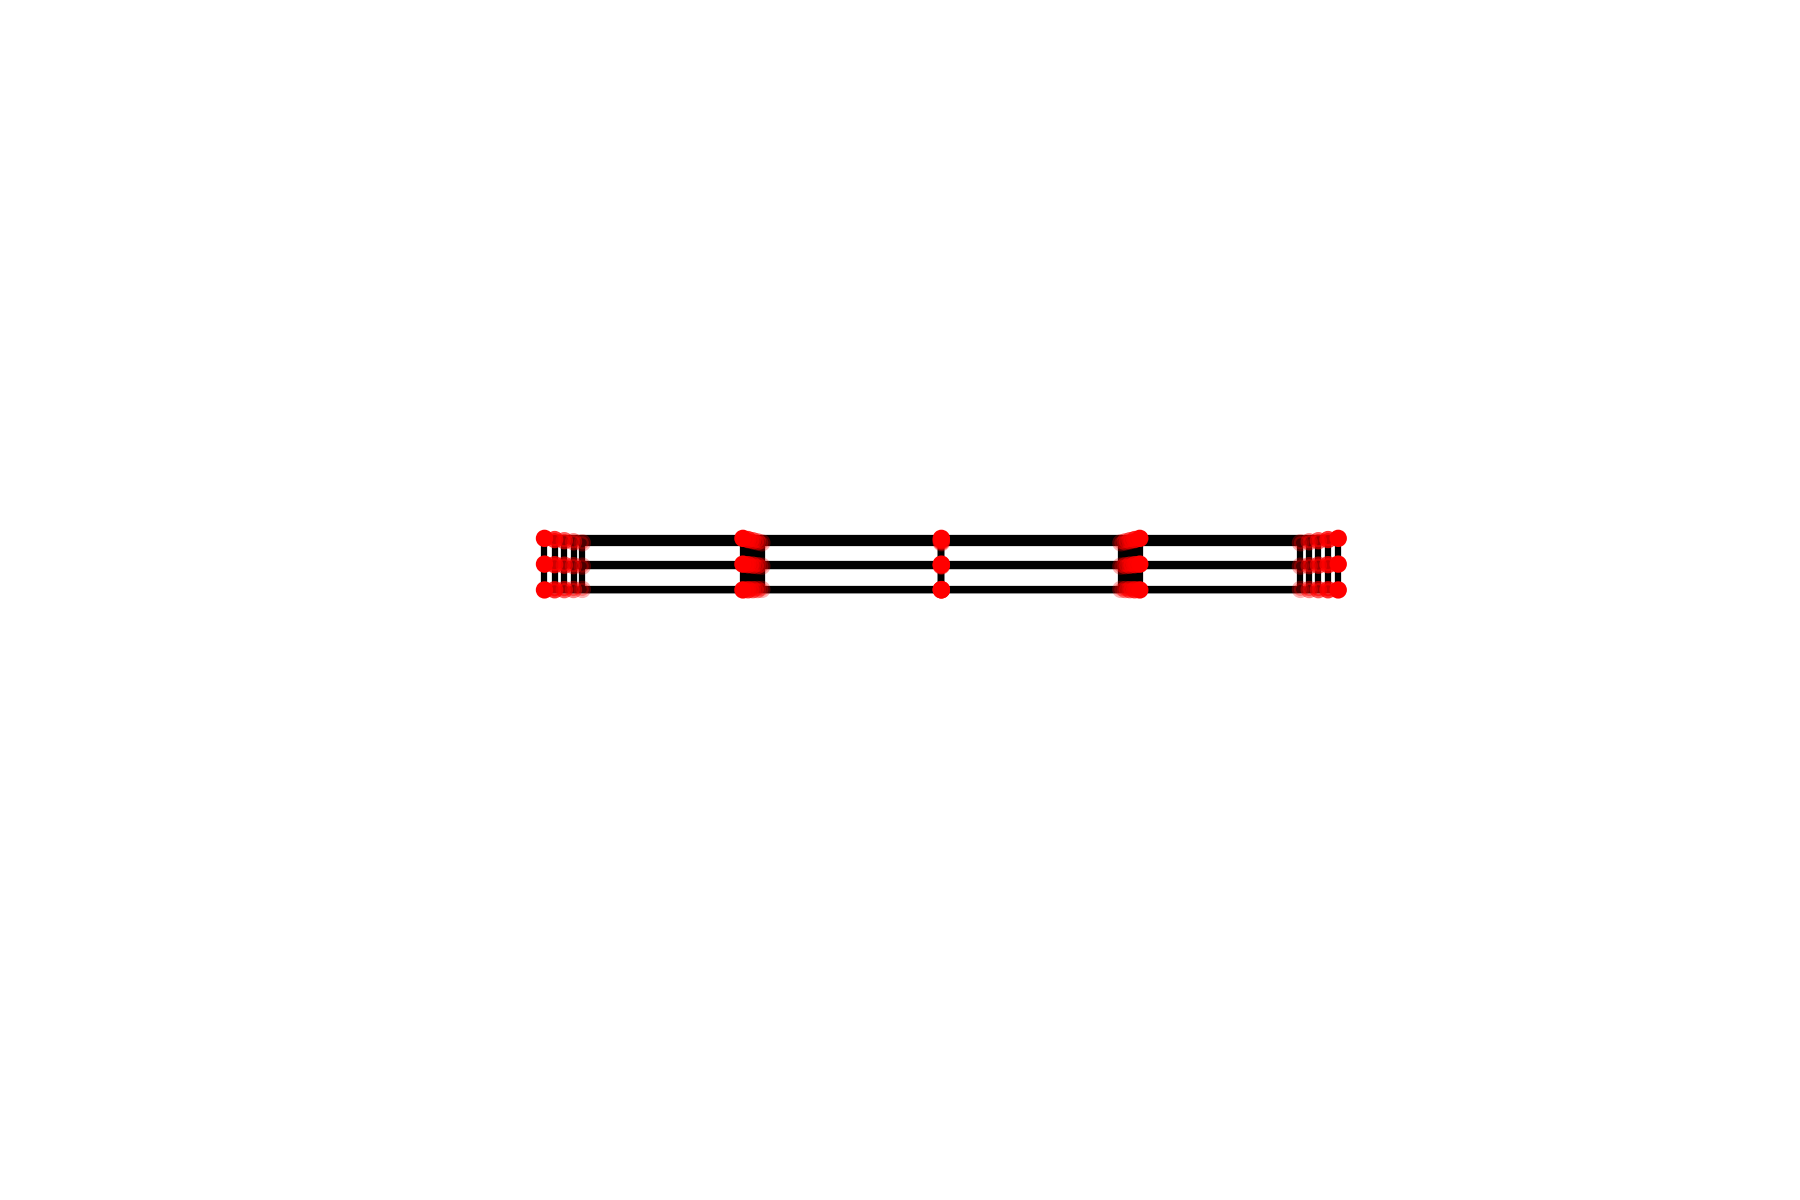
\includegraphics[width = 1\textwidth]{Figures/M1_type_a_YZ.png}
    \caption{Model 1 - Type A - YZ Projection}
    \label{fig:M1_a_YZ}
\end{minipage}
\hspace{5mm}
\begin{minipage}{0.3\textwidth}
    \centering
    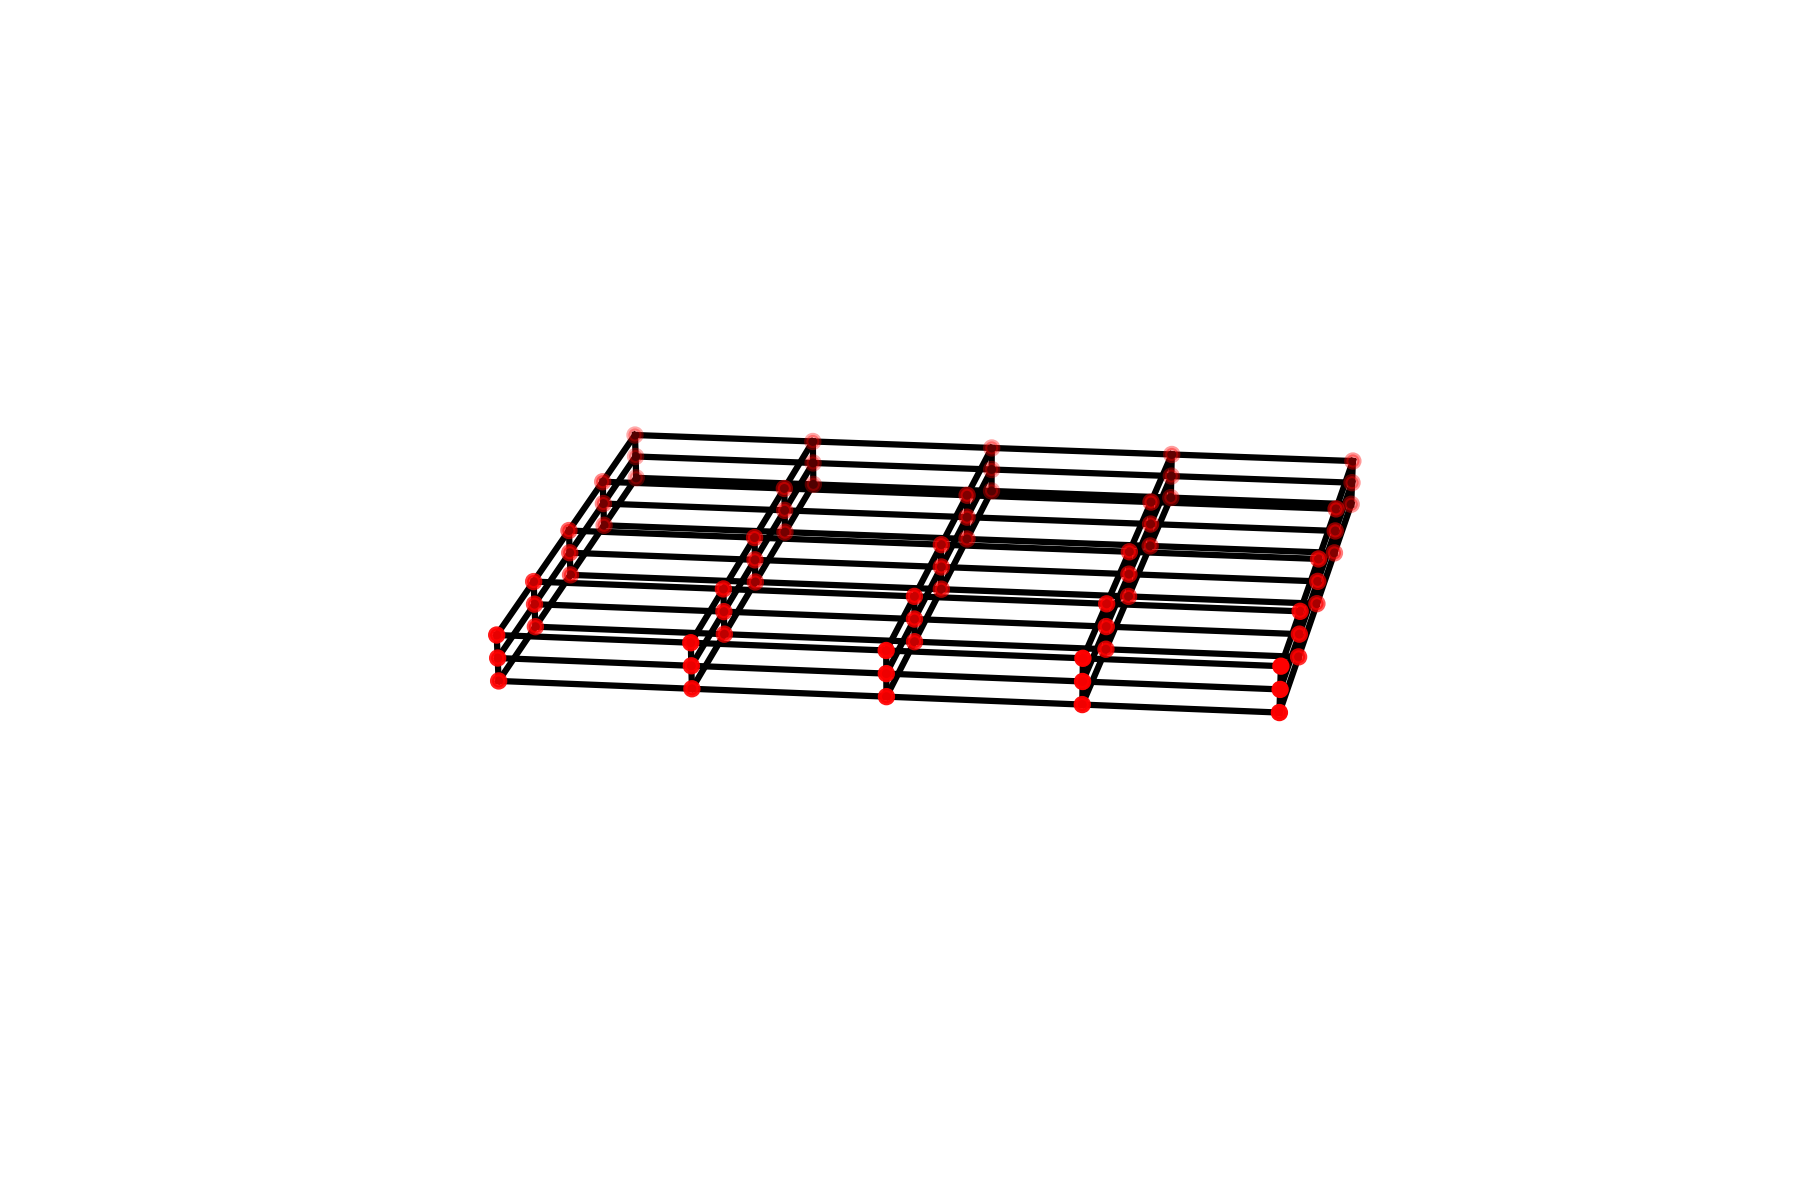
\includegraphics[width = 1\textwidth]{Figures/M1_type_a_3D.png}
    \caption{Model 1 - Type A - 3D View}
    \label{fig:M1_a_3D}
\end{minipage}
\end{figure}

The plots for vertical deflections at centre with respect to point load applied at the centre for Constant Stiffness and Constant Axial rigidity are shown in the fig~\ref{fig:M1_a_plt}.

\begin{figure}[!htbp]
    \centering
    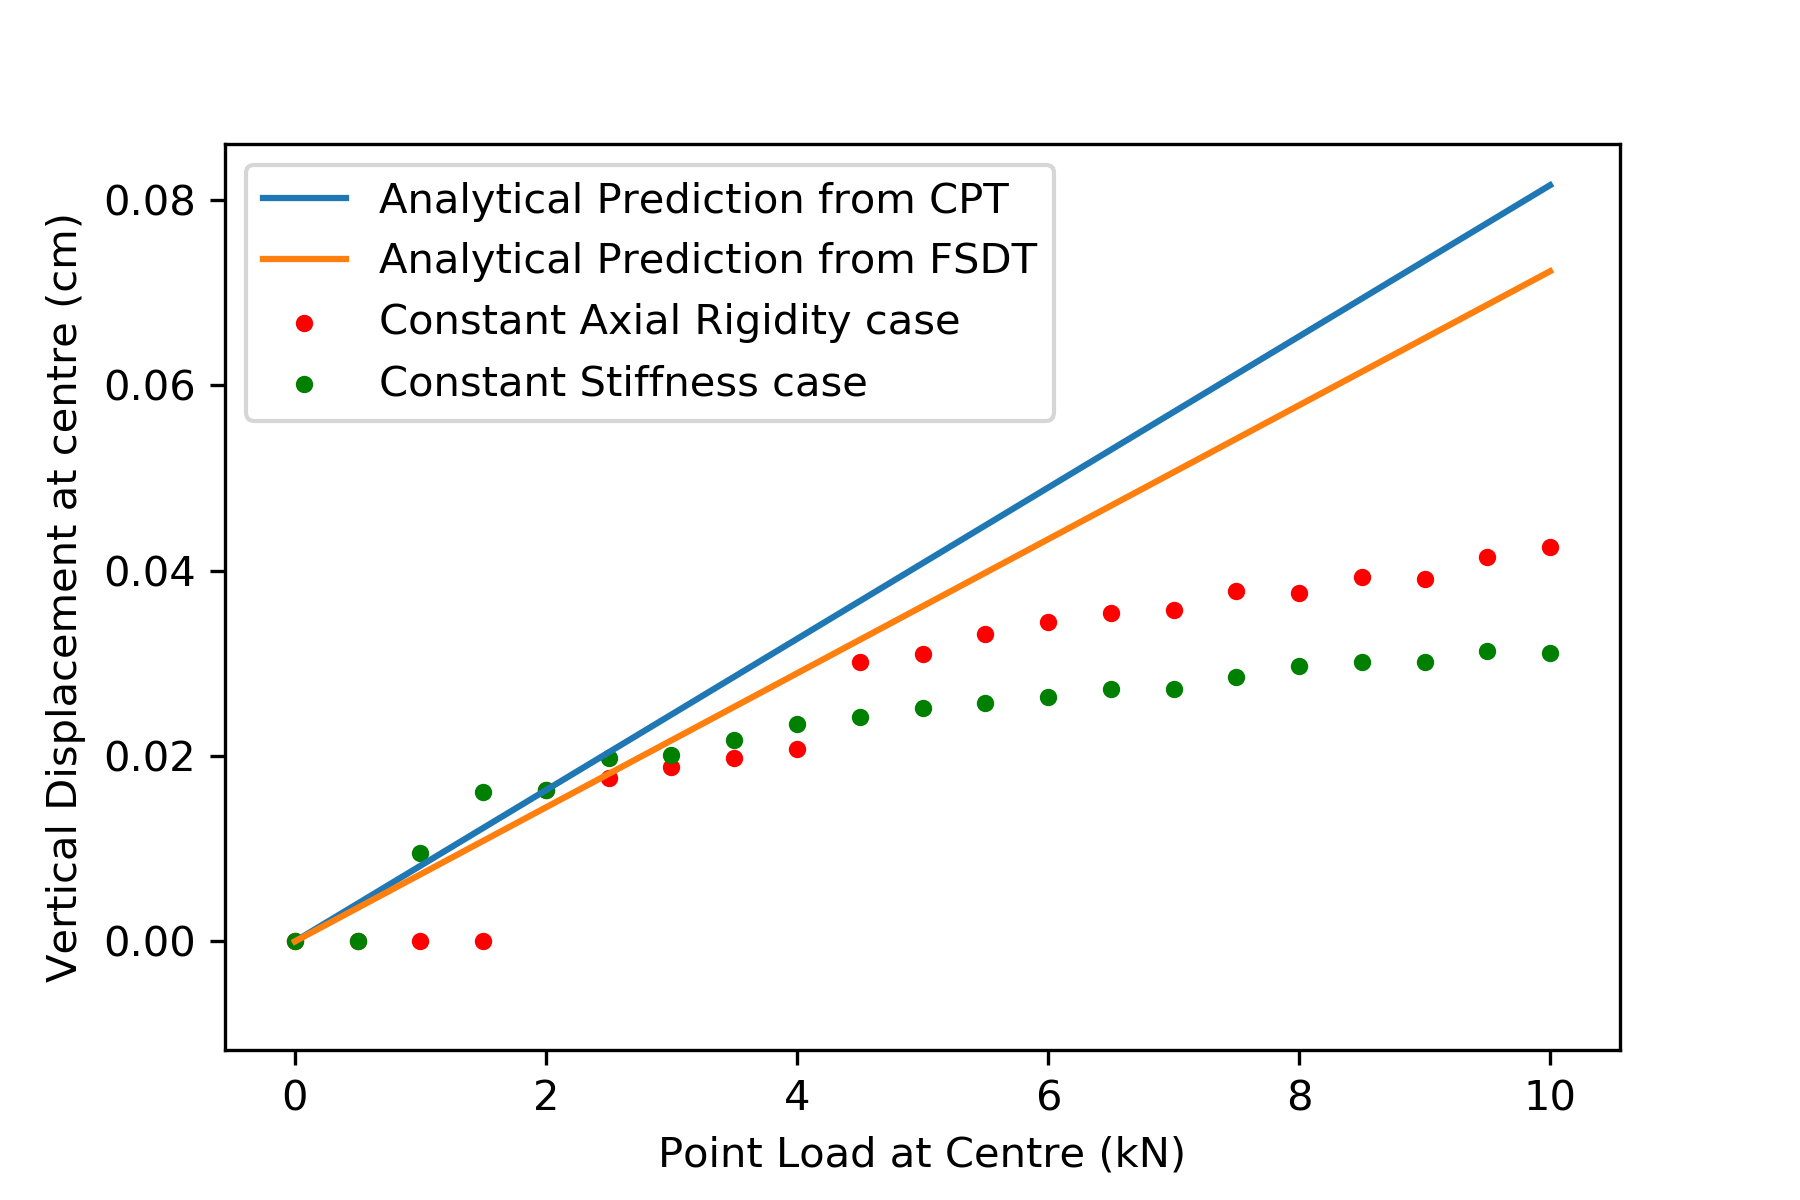
\includegraphics[width = 0.9\textwidth]{Figures/M1_a_plt.png}
    \caption{Model 1 - Type A - vertical Displacement with respect to Point Load at centre}
    \label{fig:M1_a_plt}
\end{figure}

\begin{figure}[!htbp]
    \centering
    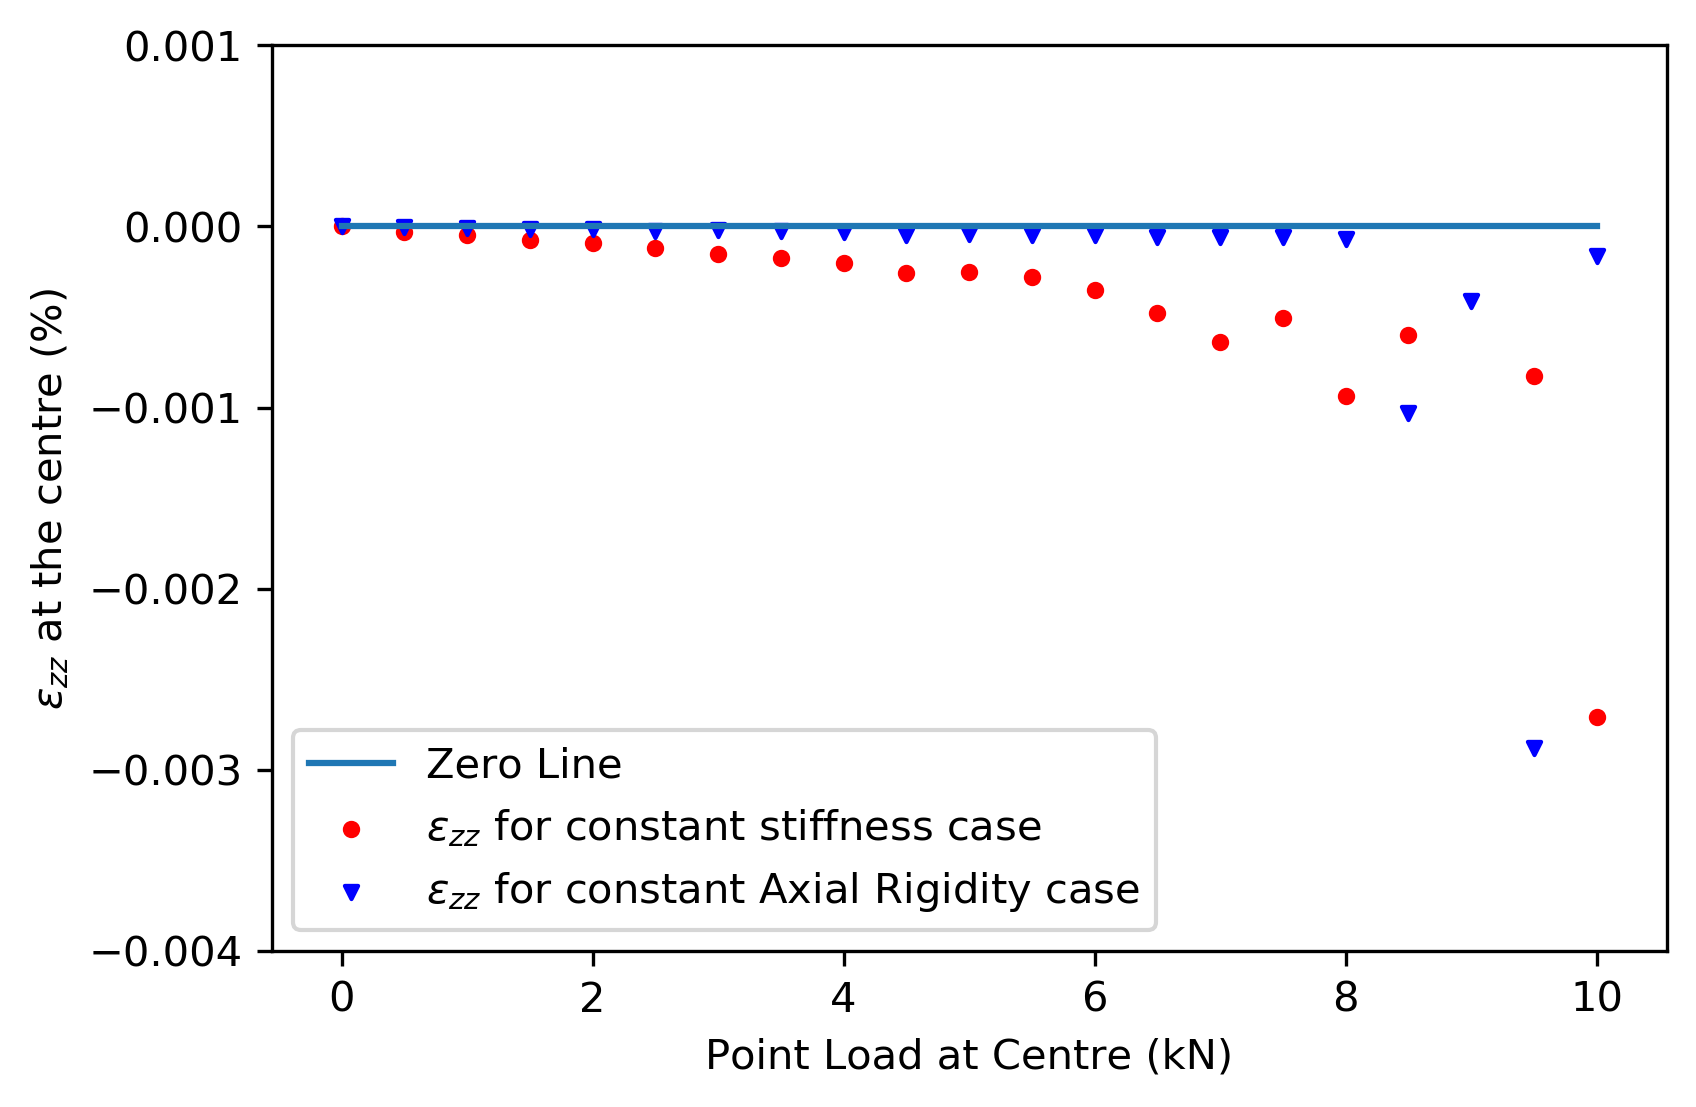
\includegraphics[width = 0.9\textwidth]{Figures/M1_a_strain.png}
    \caption{Model 1 - Type A - $\epsilon_{zz}$ with respect to Point Load at centre}
    \label{fig:M1_a_strain_plt}
\end{figure}

As it can be seen from the fig~\ref{fig:M1_a_plt}, there are significant deviations from the analytical results. The zero initial values corresponding to lower load are due to numerical difficulties in which the values in the associated matrices differ by order of magnitude and as a result are ill conditioned. This results in almost singular matrices which lead to zero displacements even when the load is applied. Also, the model underestimates the displacements at larger force magnitudes, and the predictions lie closer to the analytical solution obtained by First-order Shear Deformation Theory (FSDT) than Classical Plate Theory (CPT). This behavior can be attributed to the deviation of $\epsilon_{zz}$ from zero values (eq~\ref{eq:CPT_strains_last} and eq~\ref{eq:strain_z_FSDT} as shown in fig~\ref{fig:M1_a_strain_plt}, and non linear behavior (reaction response) of horizontal spring system as they undergo displacements in vertical direction.
%see if this can be included in appendix

\begin{figure}[!htbp]
    \centering
    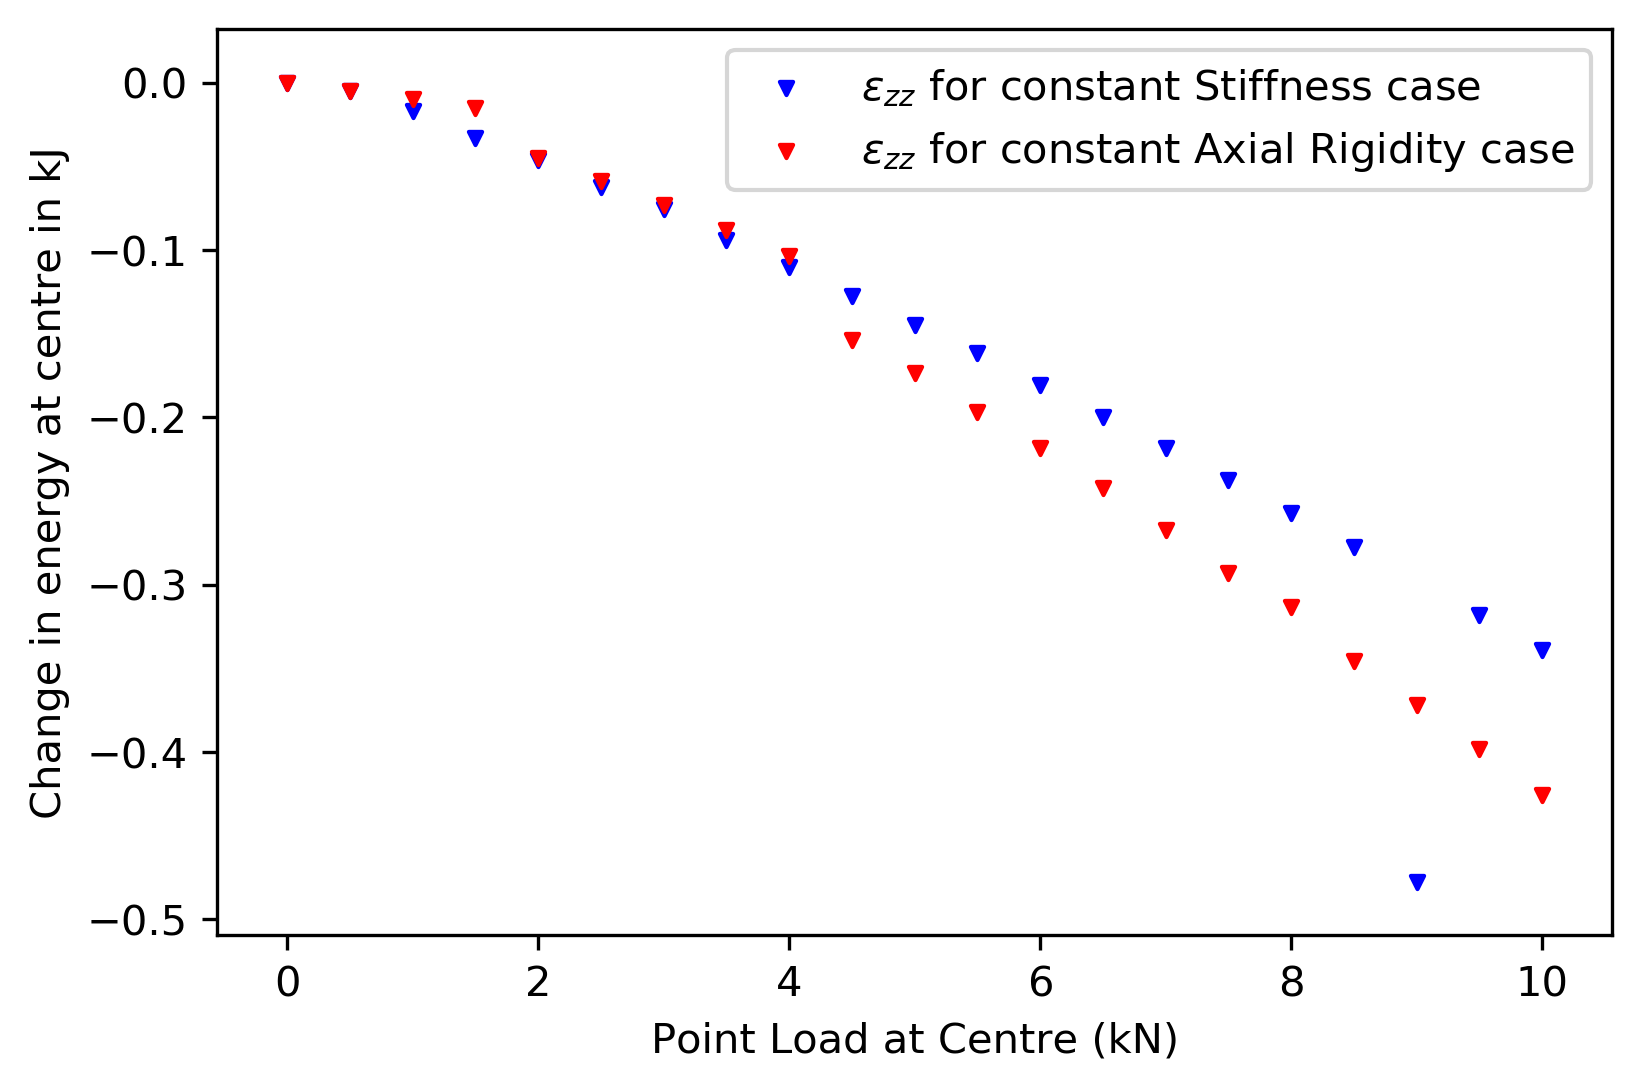
\includegraphics[width = 0.9\textwidth]{Figures/M1_a_energy.png}
    \caption{Model 1 - Type A - Change in Energy with respect to Point Load at centre}
    \label{fig:M1_a_energy}
\end{figure}

In fig~\ref{fig:M1_a_energy}, energies in the undeformed states for all forces are zero.

\subsubsection{Model 1 - Type B}
Model 1 - Type B is 10 x 10 x 2 structure of Model 1 cuboids of dimensions 0.1~m x 0.1~m x 0.01~m. The model is shown in fig~\ref{fig:M1_b_XY} - fig~\ref{fig:M1_b_3D}

\begin{figure}[!htbp]
\begin{minipage}{0.3\textwidth}
    \centering
    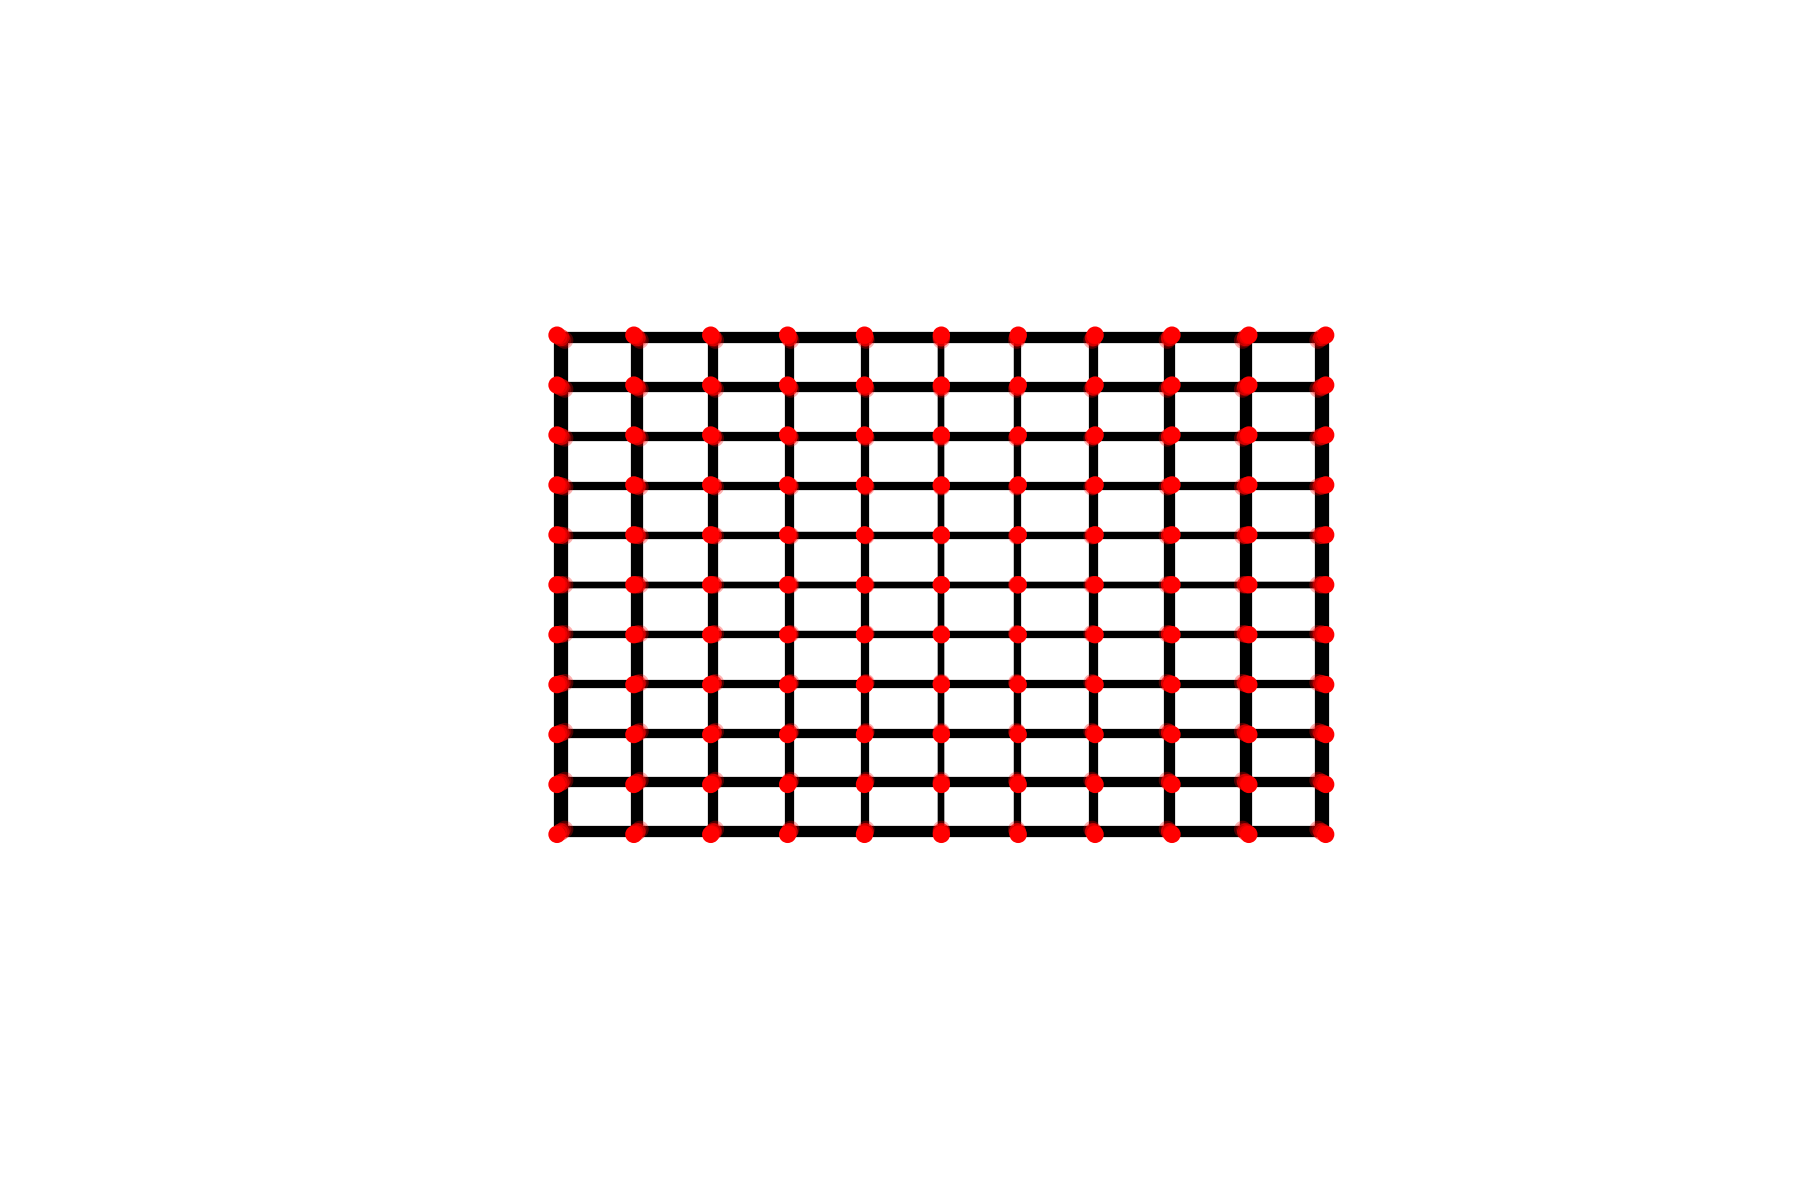
\includegraphics[width = 1\textwidth]{Figures/M1_b_XY.png}
    \caption{Model 1 - Type B - XY Projection}
    \label{fig:M1_b_XY}
\end{minipage}
\hspace{5mm}
\begin{minipage}{0.3\textwidth}
    \centering
    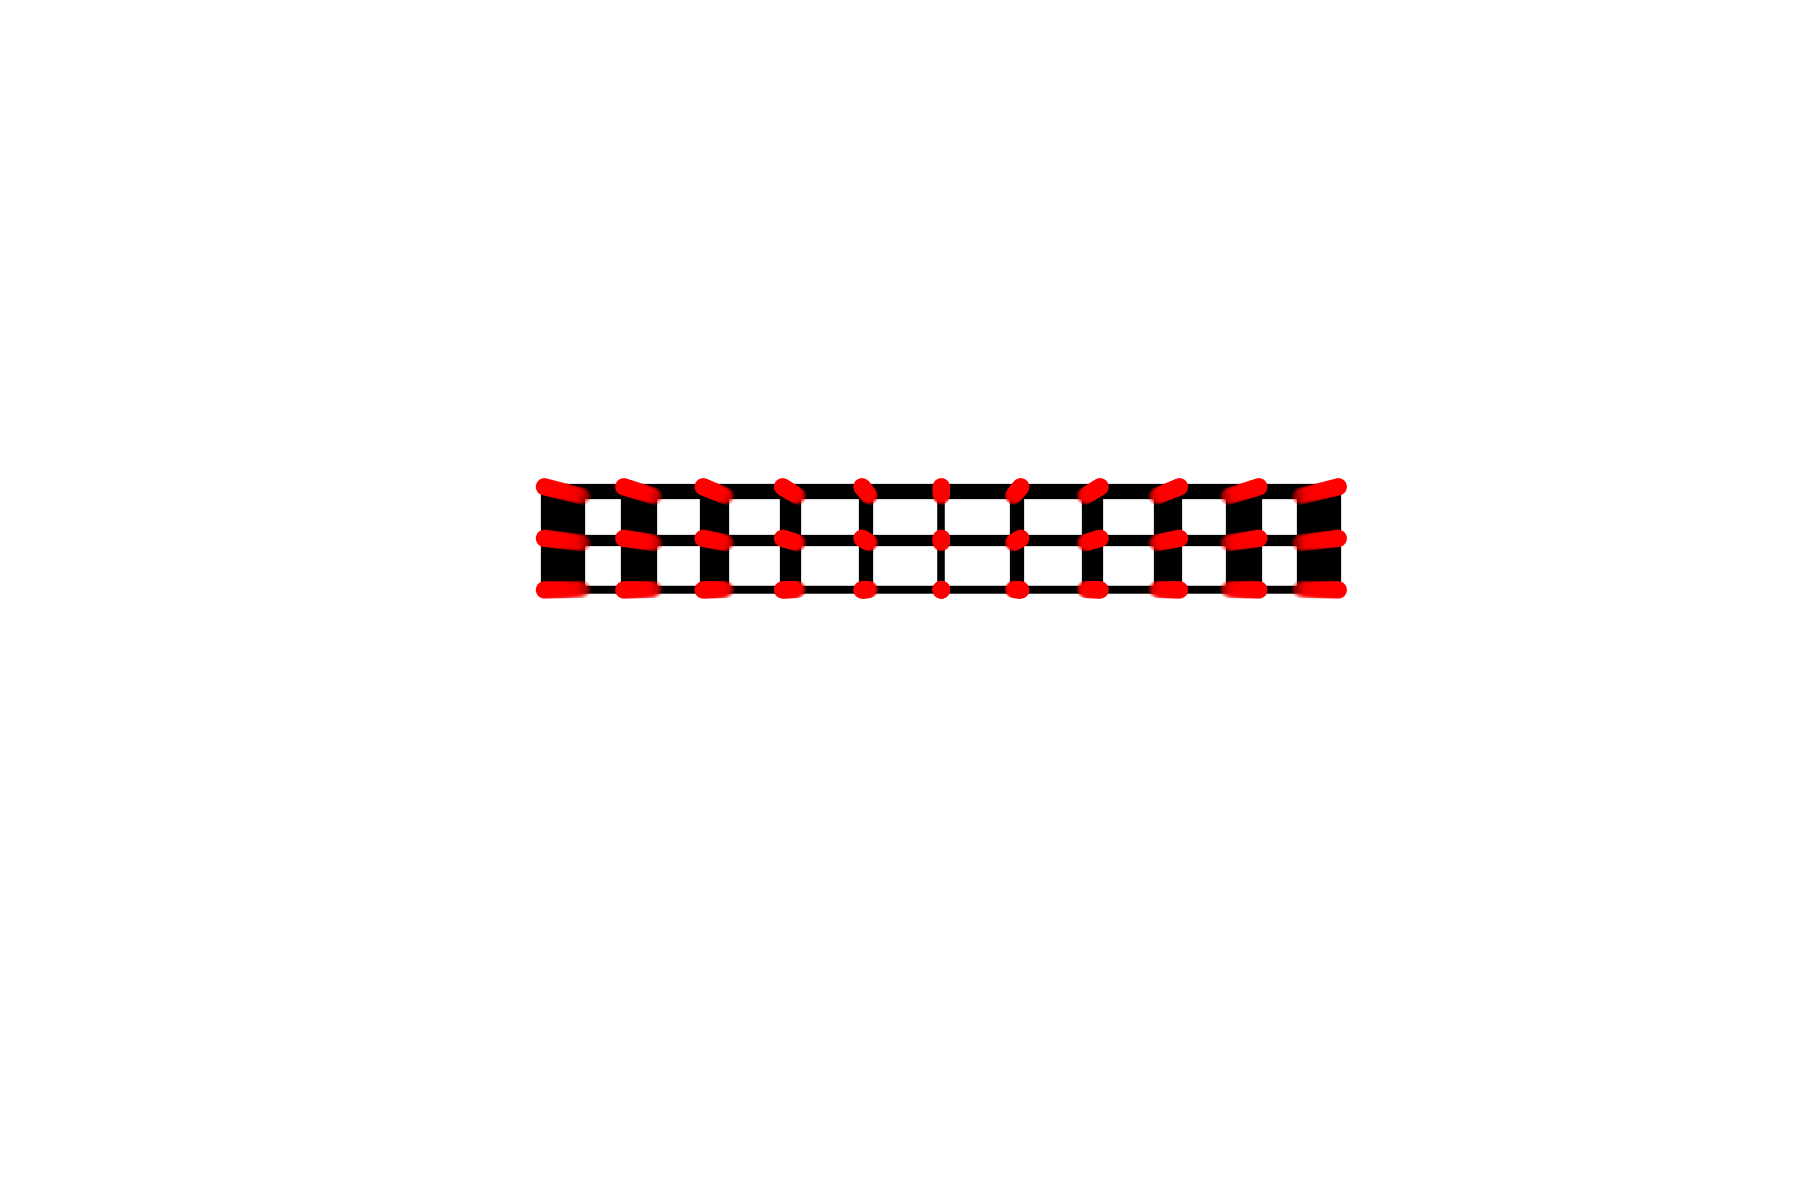
\includegraphics[width = 1\textwidth]{Figures/M1_b_YZ.png}
    \caption{Model 1 - Type B - YZ Projection}
    \label{fig:M1_b_YZ}
\end{minipage}
\hspace{5mm}
\begin{minipage}{0.3\textwidth}
    \centering
    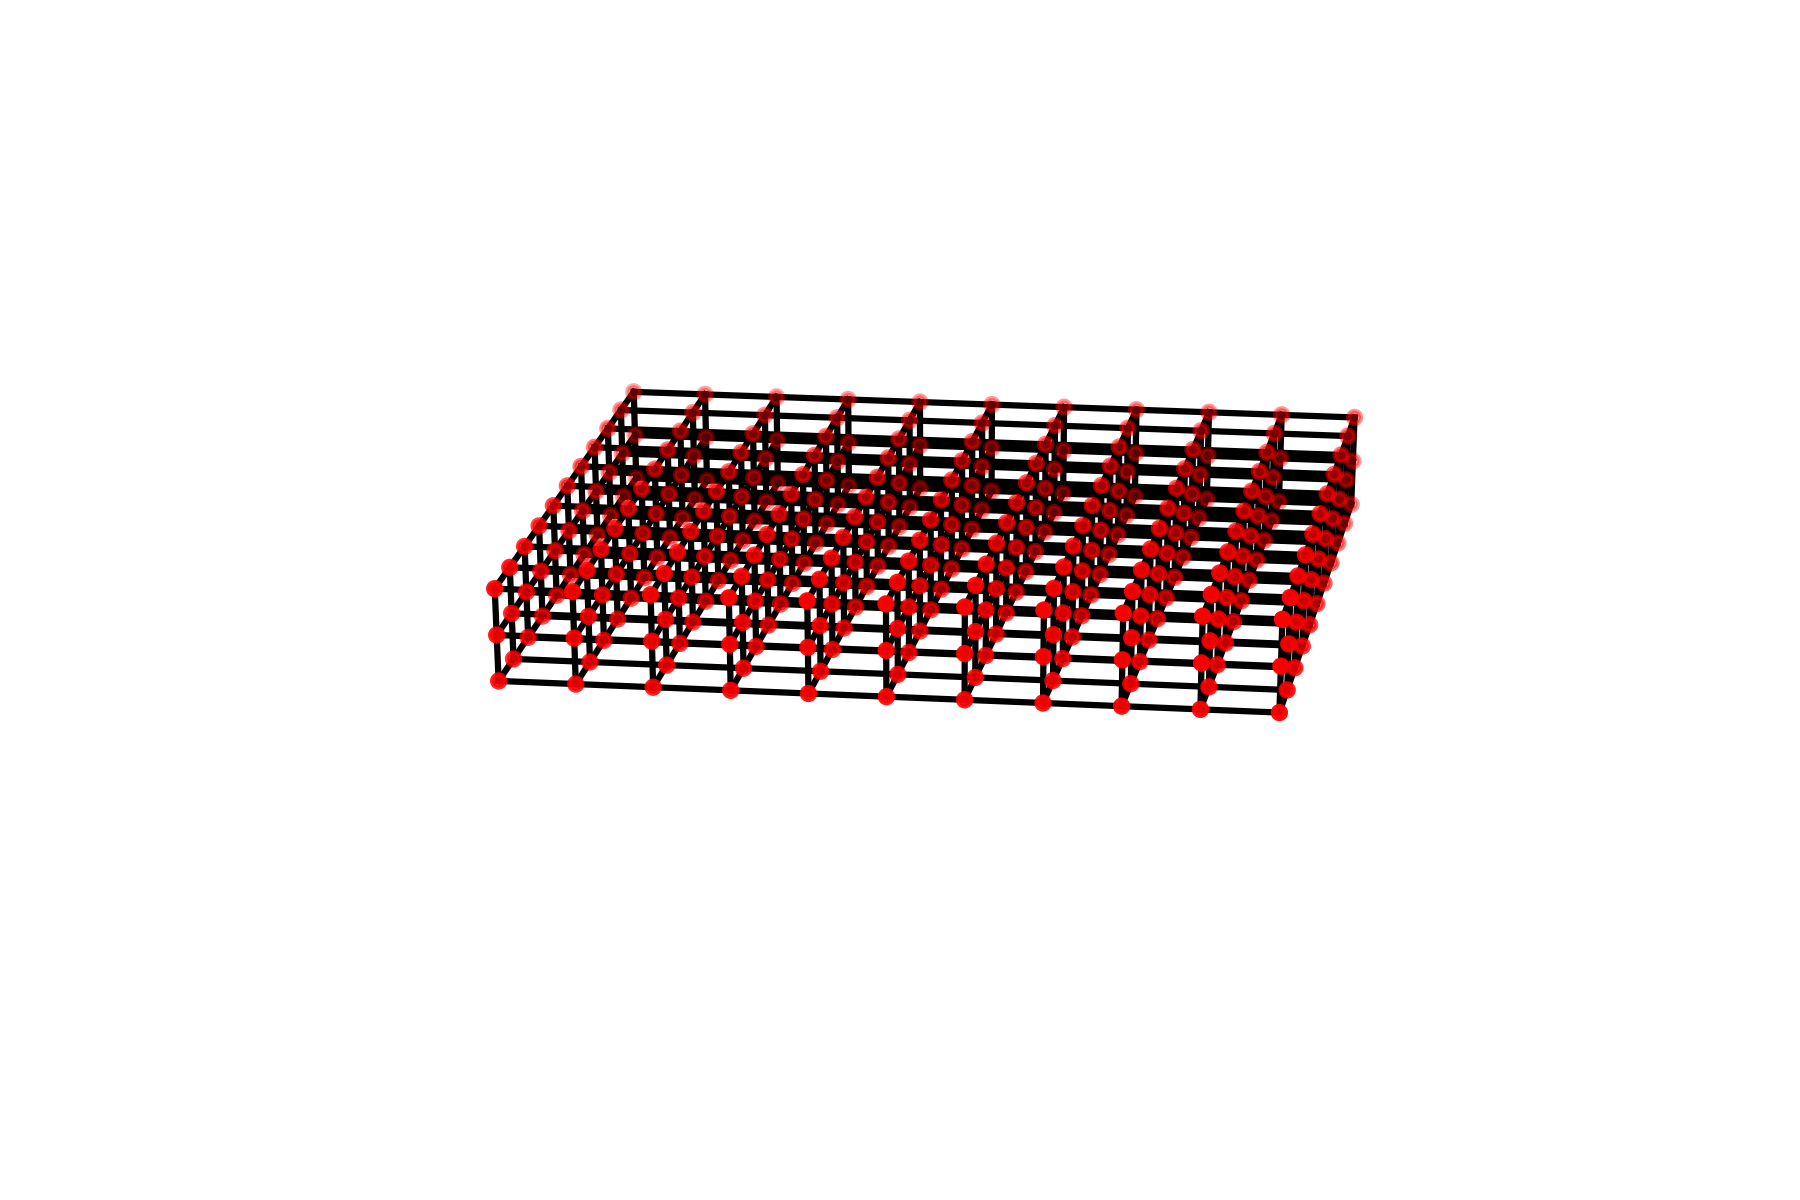
\includegraphics[width = 1\textwidth]{Figures/M1_b_3D.png}
    \caption{Model 1 - Type B - 3D View}
    \label{fig:M1_b_3D}
\end{minipage}
\end{figure}

The plots corresponding to Model 1 - Type B are shown in fig~\ref{fig:M1_b_plt} - fig~\ref{fig:M1_b_energy}.

\begin{figure}[!htbp]
    \centering
    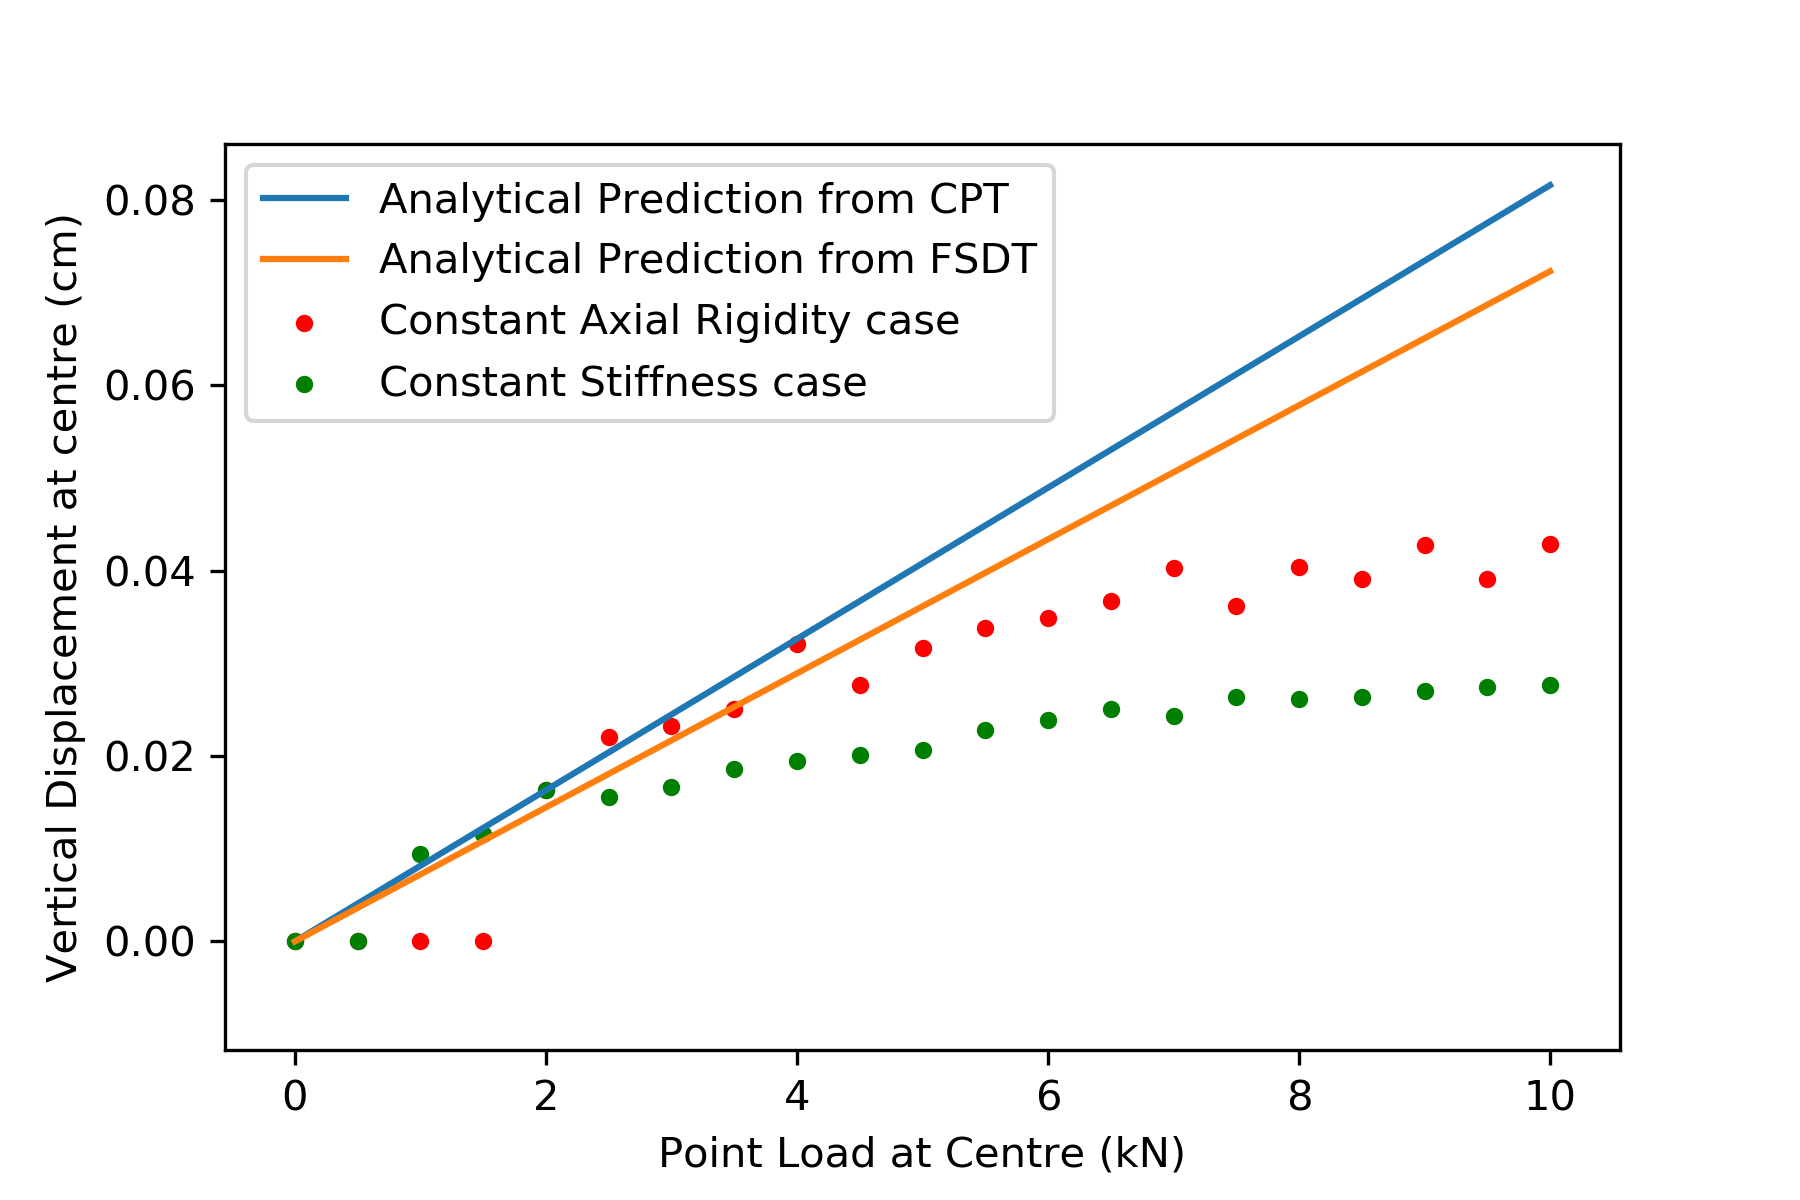
\includegraphics[width = 0.8\textwidth]{Figures/M1_b_plt.png}
    \caption{Model 1 - Type B - vertical Displacement with respect to Point Load at centre}
    \label{fig:M1_b_plt}
\end{figure}

\begin{figure}[!htbp]
    \centering
    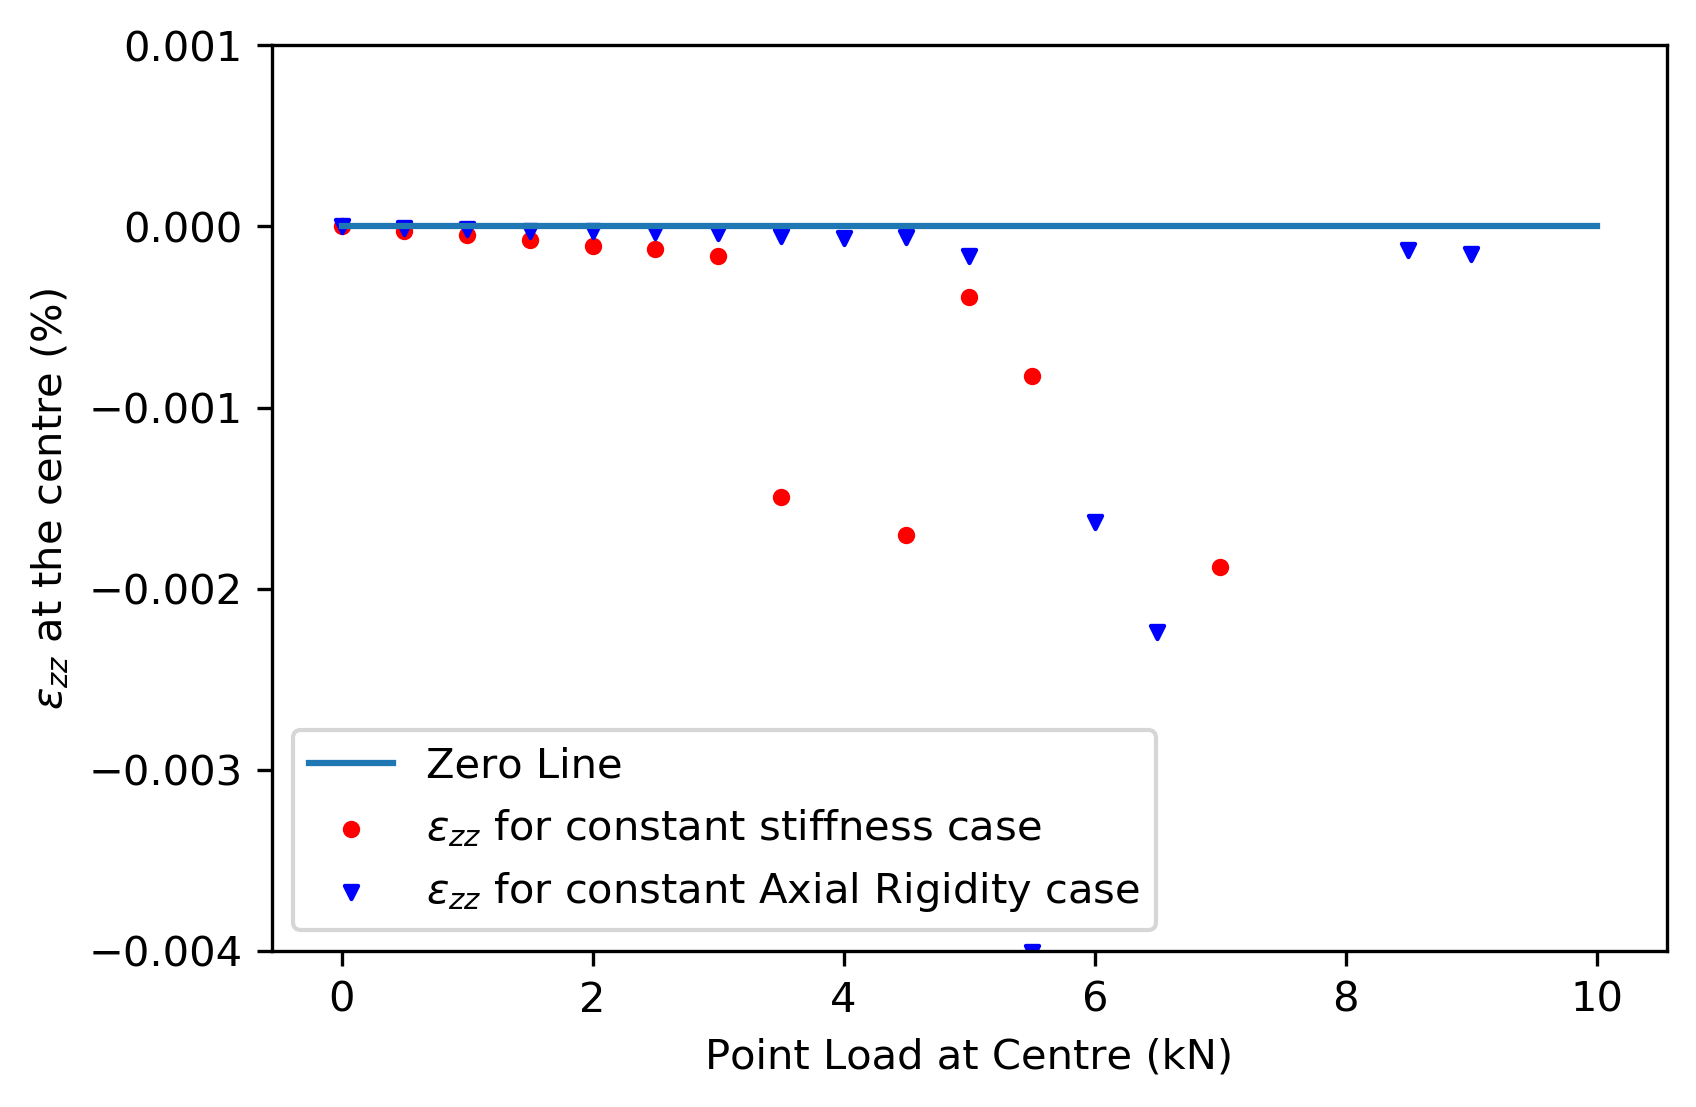
\includegraphics[width = 0.9\textwidth]{Figures/M1_b_strain.png}
    \caption{Model 1 - Type B - $\epsilon_{zz}$ with respect to Point Load at centre}
    \label{fig:M1_b_strain_plt}
\end{figure}

Type B Model follows the analytical predictions for displacement more closely as compared to Type A as evident from the fig~\ref{fig:M1_b_plt}. Among the two study cases, Constant Axial Rigidity model provides better results compared to Constant Stiffness model. The normal strain in Z-direction $\epsilon_{zz}$ obtained from the model is quite erratic for loads higher than 3 kN for constant Stiffness case and loads higher than 5.5 kN for constant Axial Rigidity case as shown in the fig~\ref{fig:M1_b_strain_plt}. Some of the points not shown in fig~\ref{fig:M1_b_strain_plt} correspond to very high strain resulting from complete crushing of the vertical springs at centre under the load as shown in fig~\ref{fig:crushed_M1_b}.


\begin{figure}[!htbp]
    \centering
    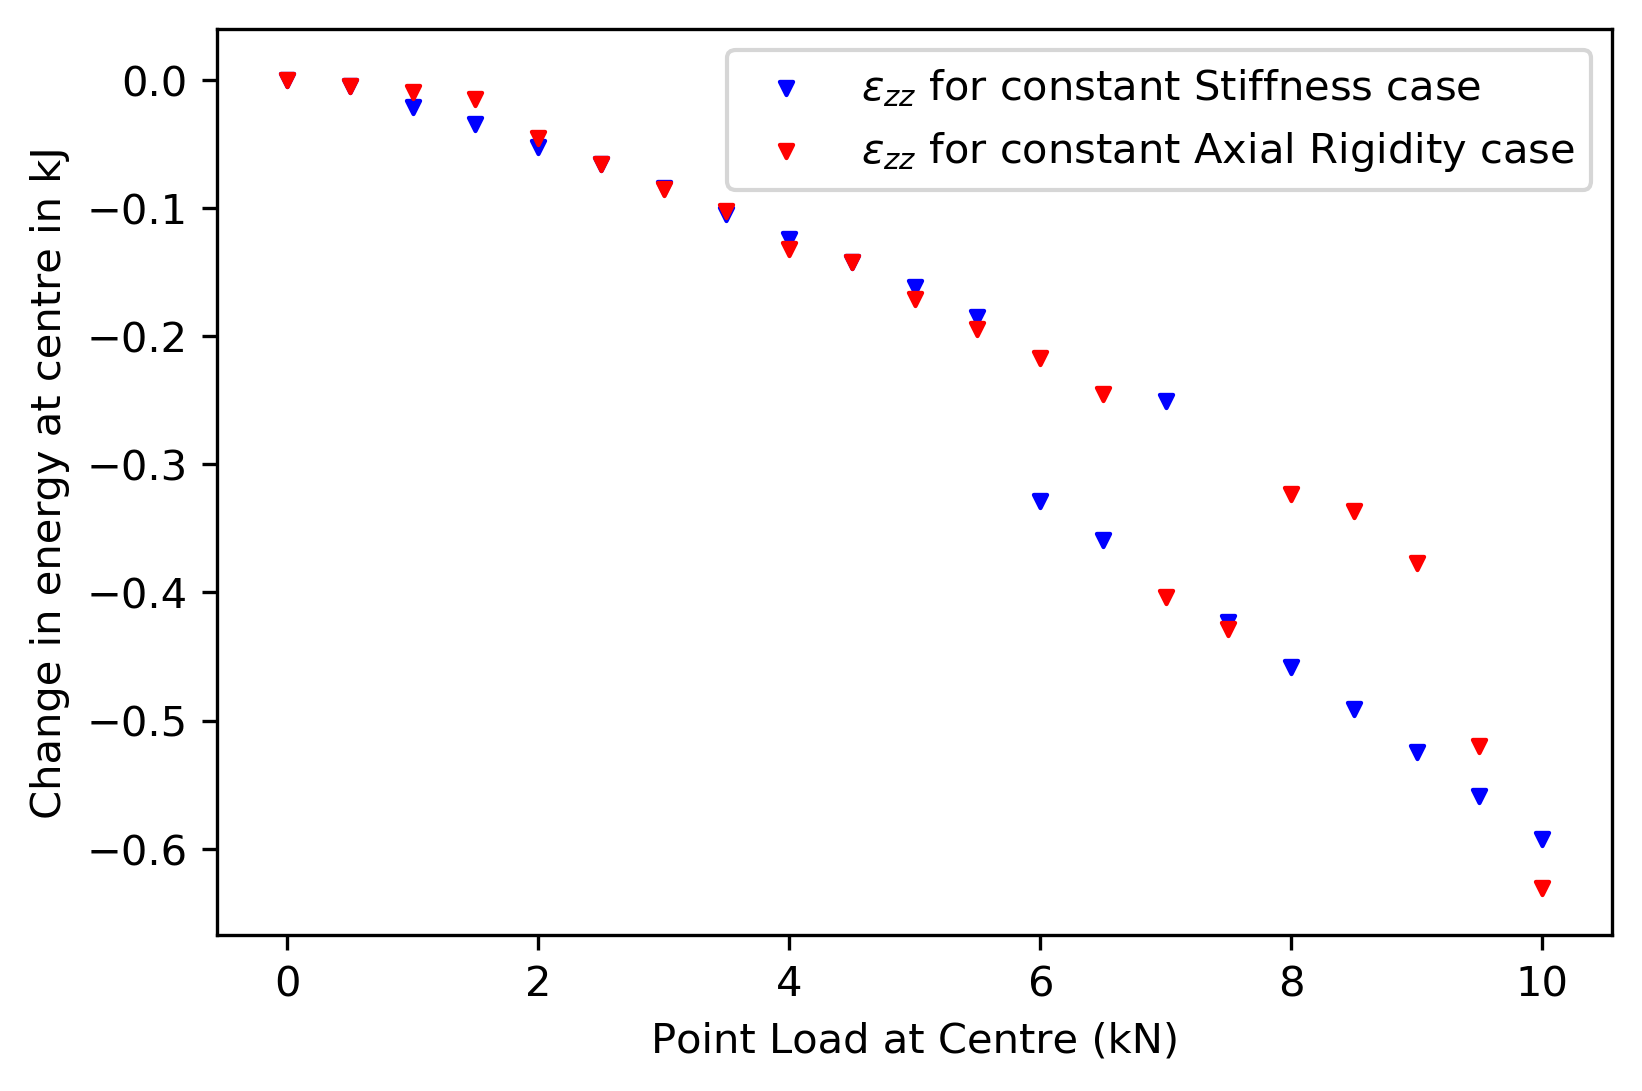
\includegraphics[width = 0.9\textwidth]{Figures/M1_b_energy.png}
    \caption{Model 1 - Type B - Change in Energy with respect to Point Load at centre}
    \label{fig:M1_b_energy}
\end{figure}

In fig~\ref{fig:M1_b_energy}, energies in the undeformed states for all forces are zero.

\begin{figure}[!htbp]
    \centering
    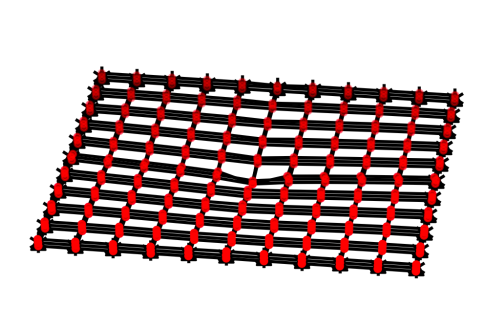
\includegraphics[width = 0.6\textwidth]{Figures/crushed_M1_b.png}
    \caption{Model 1 - Type B - Crushed vertical springs under loading of 8 kN resulting in very high $\epsilon_{zz}$}
    \label{fig:crushed_M1_b}
\end{figure}

 From fig~\ref{fig:M1_b_energy}, we can see that there is a discontinuity in energy profile for Constant Stiffness case at around load of 6 kN, Some irregularities are also present in energy variation of both the cases. Interestingly, for Constant Axial Rigidity case, the point where there is a discontinuity in energy field (around 6 kN) is the same point at which the predictions for vertical displacements start deviating from the analytical results obtained from First-order Shear Deformation theory and strains turn sporadic, even though energies after discontinuity in energy profiles are lower compared to the energies at the same loading if they continued the earlier pattern. This suggests a sharp change in the properties of the model or some kind of instability which leads to such results. 
 
 \subsubsection{Model 1 - Type C}
 Model 1 - Type C is 20 x 20 x 2 structure of Model 1 cuboids of dimensions 0.05~m x 0.05~m x 0.01~m. The model is shown in fig~\ref{fig:M1_c_XY} - fig~\ref{fig:M1_c_3D}

\begin{figure}[!htbp]
\begin{minipage}{0.3\textwidth}
    \centering
    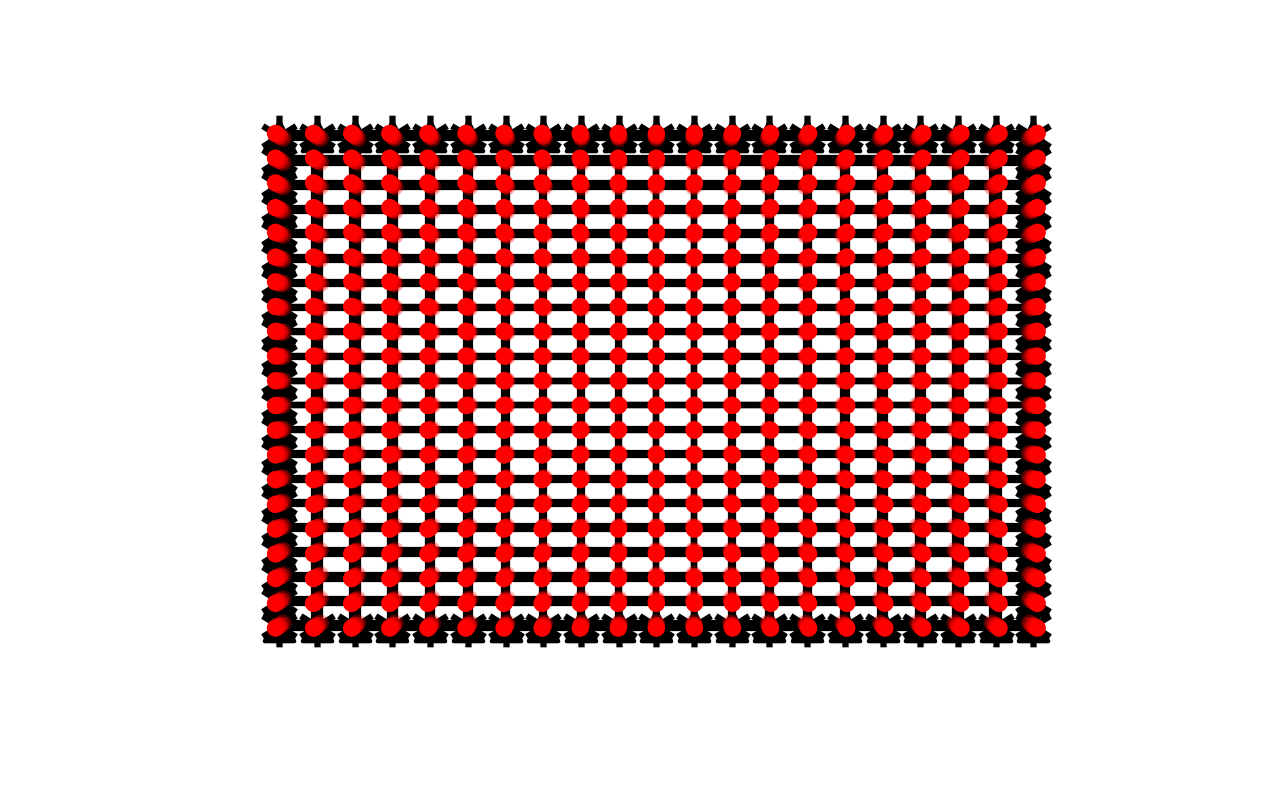
\includegraphics[width = 1\textwidth]{Figures/M1_type_c_XY.png}
    \caption{Model 1 - Type C - XY Projection}
    \label{fig:M1_c_XY}
\end{minipage}
\hspace{5mm}
\begin{minipage}{0.3\textwidth}
    \centering
    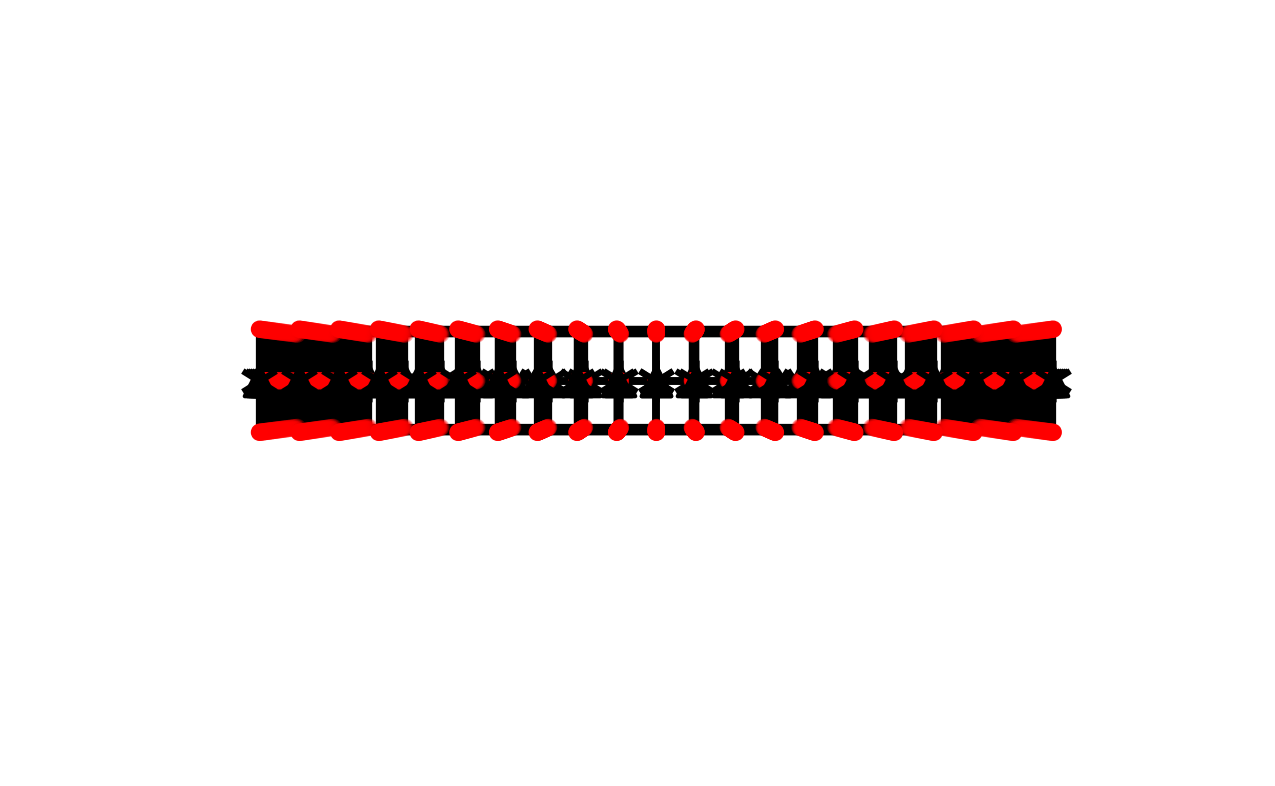
\includegraphics[width = 1\textwidth]{Figures/M1_type_c_YZ.png}
    \caption{Model 1 - Type C - YZ Projection}
    \label{fig:M1_c_YZ}
\end{minipage}
\hspace{5mm}
\begin{minipage}{0.3\textwidth}
    \centering
    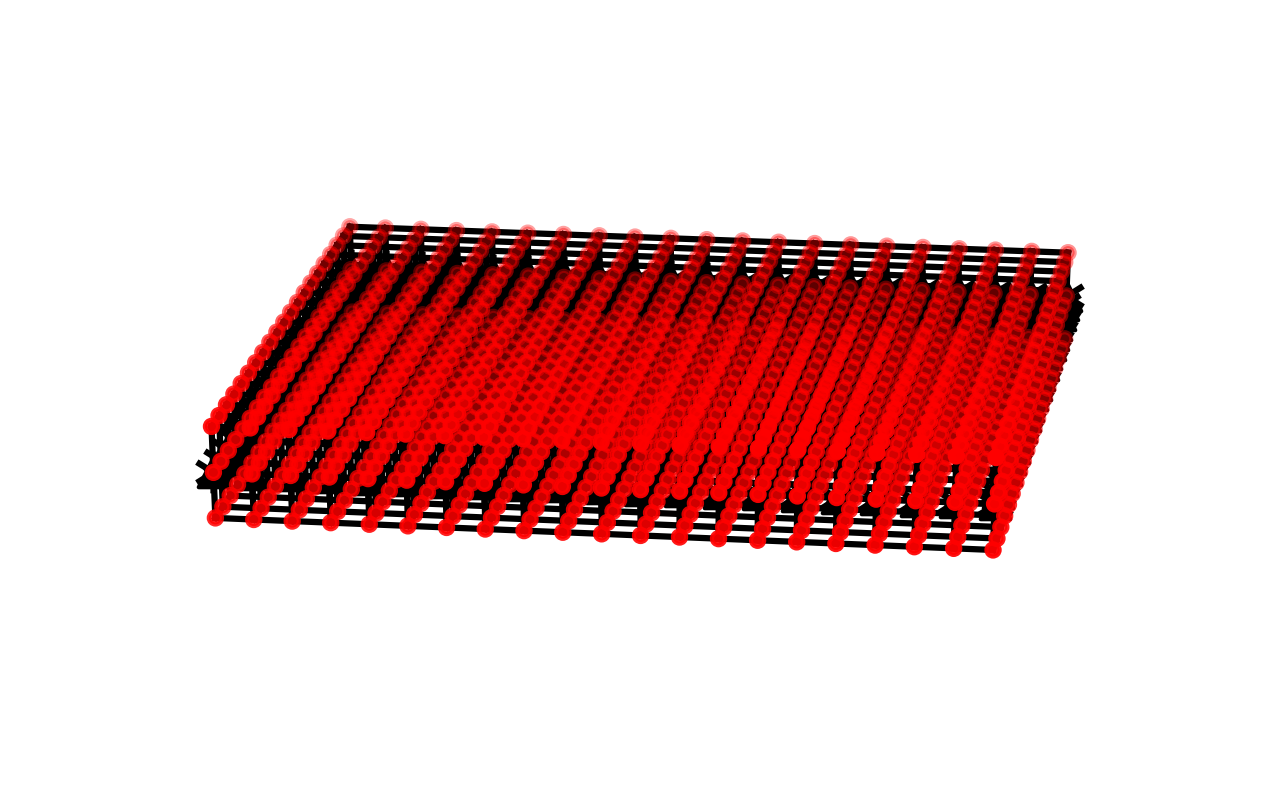
\includegraphics[width = 1\textwidth]{Figures/M1_type_c_3D.png}
    \caption{Model 1 - Type C - 3D View}
    \label{fig:M1_c_3D}
\end{minipage}
\end{figure}

The plots corresponding to Model 1 - Type C are shown in fig~\ref{fig:M1_c_plt} - fig~\ref{fig:M1_c_energy}


Model 1 - Type C predictions for vertical deflection at centre are similar to that predicted by Model 1 - Type B, however the predictions are more uniform and closely follow the analytical prediction at smaller loads. In this case both, Constant Axial Rigidity and Constant Stiffness, study predict almost similar deflection. However, unlike Model 1 - Type A and Model 1 - Type B, Constant stiffness study predicts deflection closer to analytical predictions, although marginally, compared to Constant Axial Rigidity study.

\begin{figure}[!htbp]
    \centering
    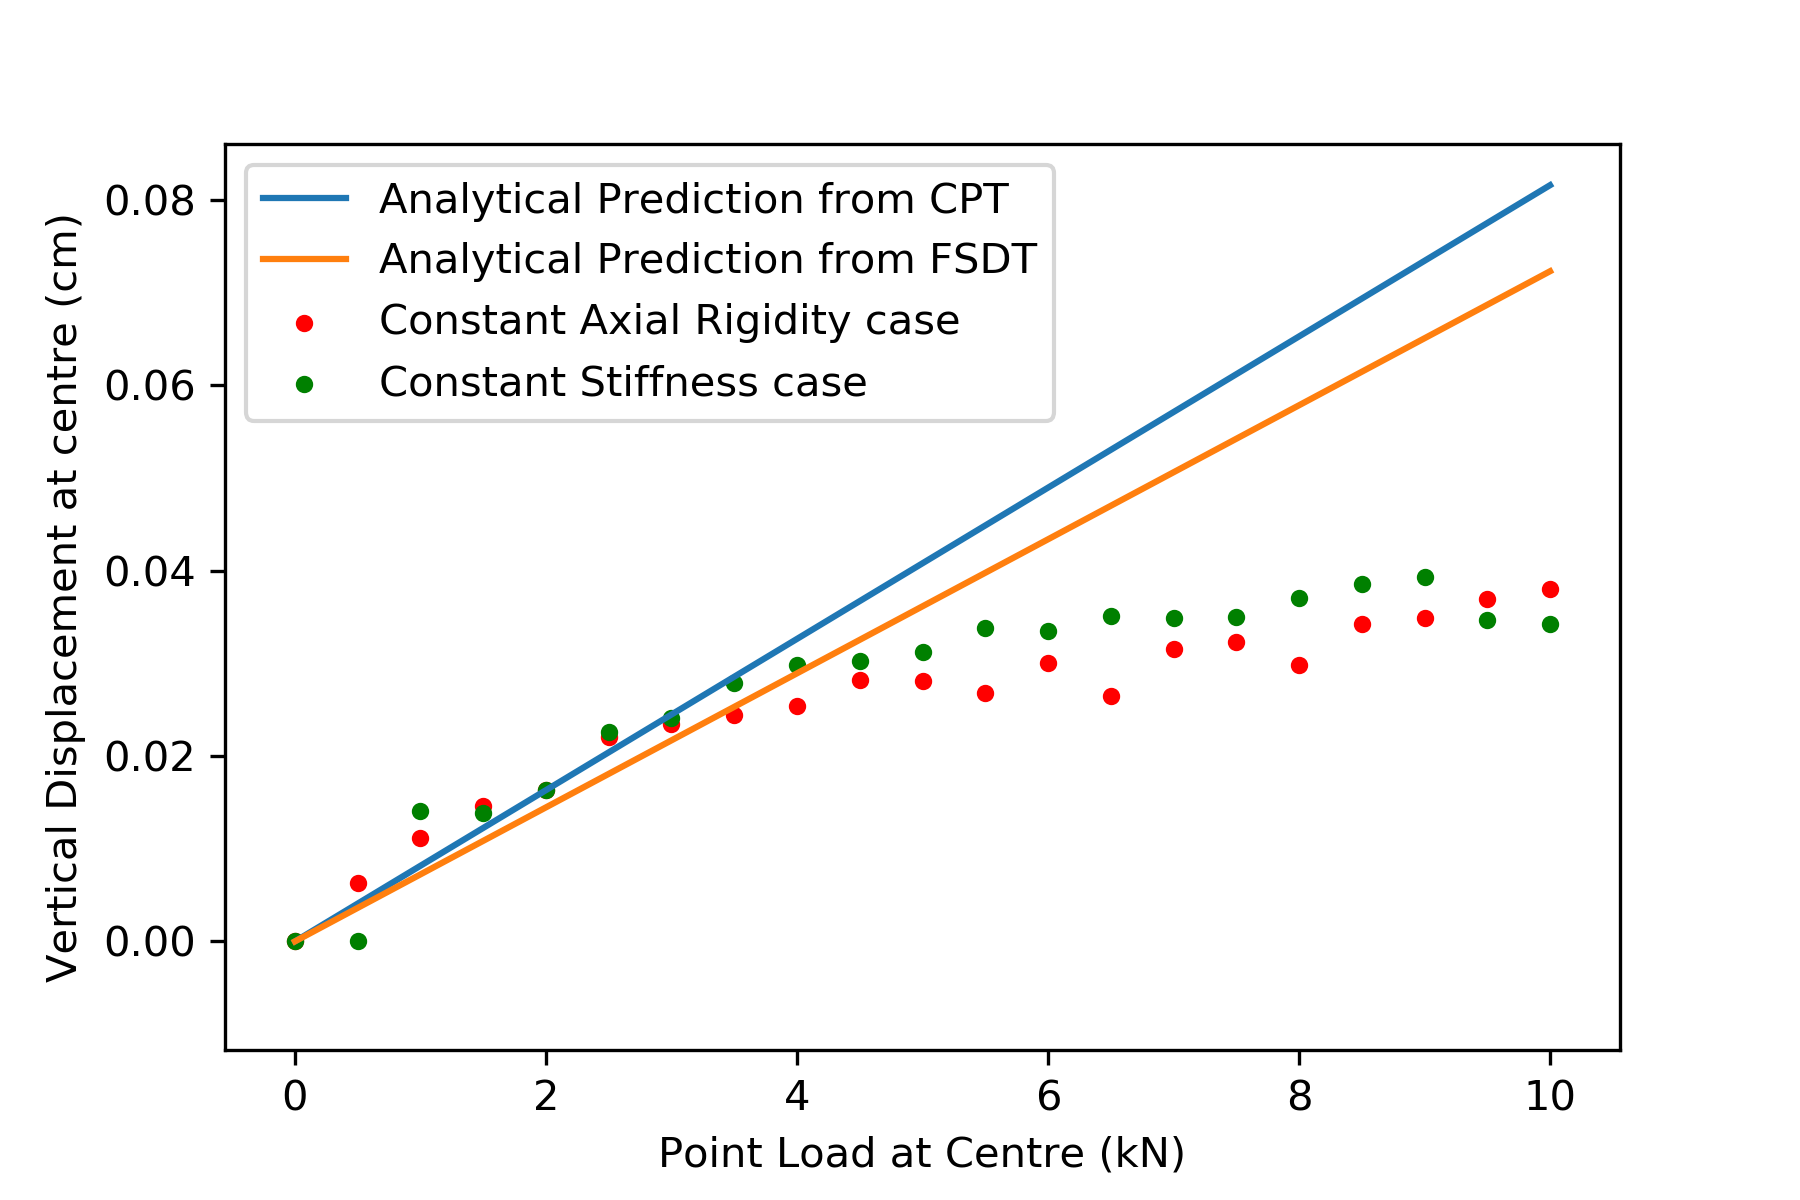
\includegraphics[width = 0.8\textwidth]{Figures/M1_c_plt.png}
    \caption{Model 1 - Type C - vertical Displacement with respect to Point Load at centre}
    \label{fig:M1_c_plt}
\end{figure}

\begin{figure}[!htbp]
    \centering
    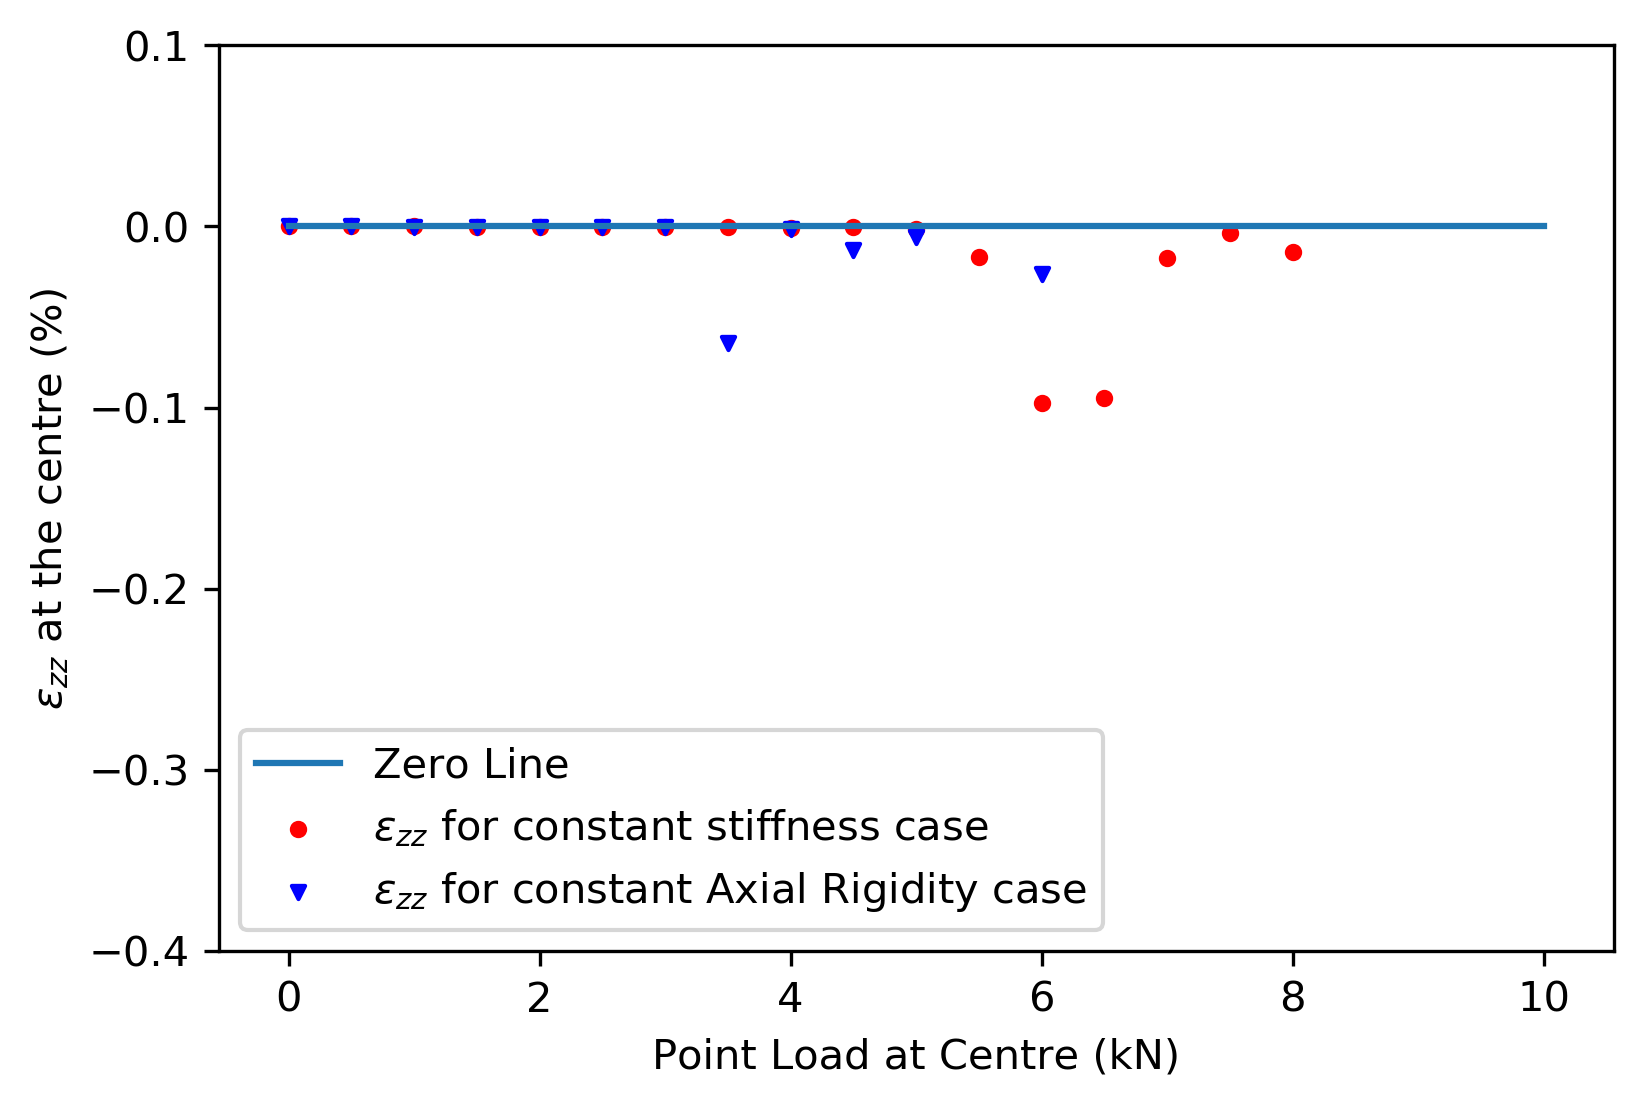
\includegraphics[width = 0.9\textwidth]{Figures/M1_c_strain.png}
    \caption{Model 1 - Type C - $\epsilon_{zz}$ with respect to Point Load at centre}
    \label{fig:M1_c_strain_plt}
\end{figure}

Strains predicted by this model are similar to those predicted by Type A and Type B models at lower load, however the vertical strains turn to be very erratic and large for higher loading. Some of the points with very high strains are not shown in the fig~\ref{fig:M1_c_strain_plt}. 

\begin{figure}[!htbp]
    \centering
    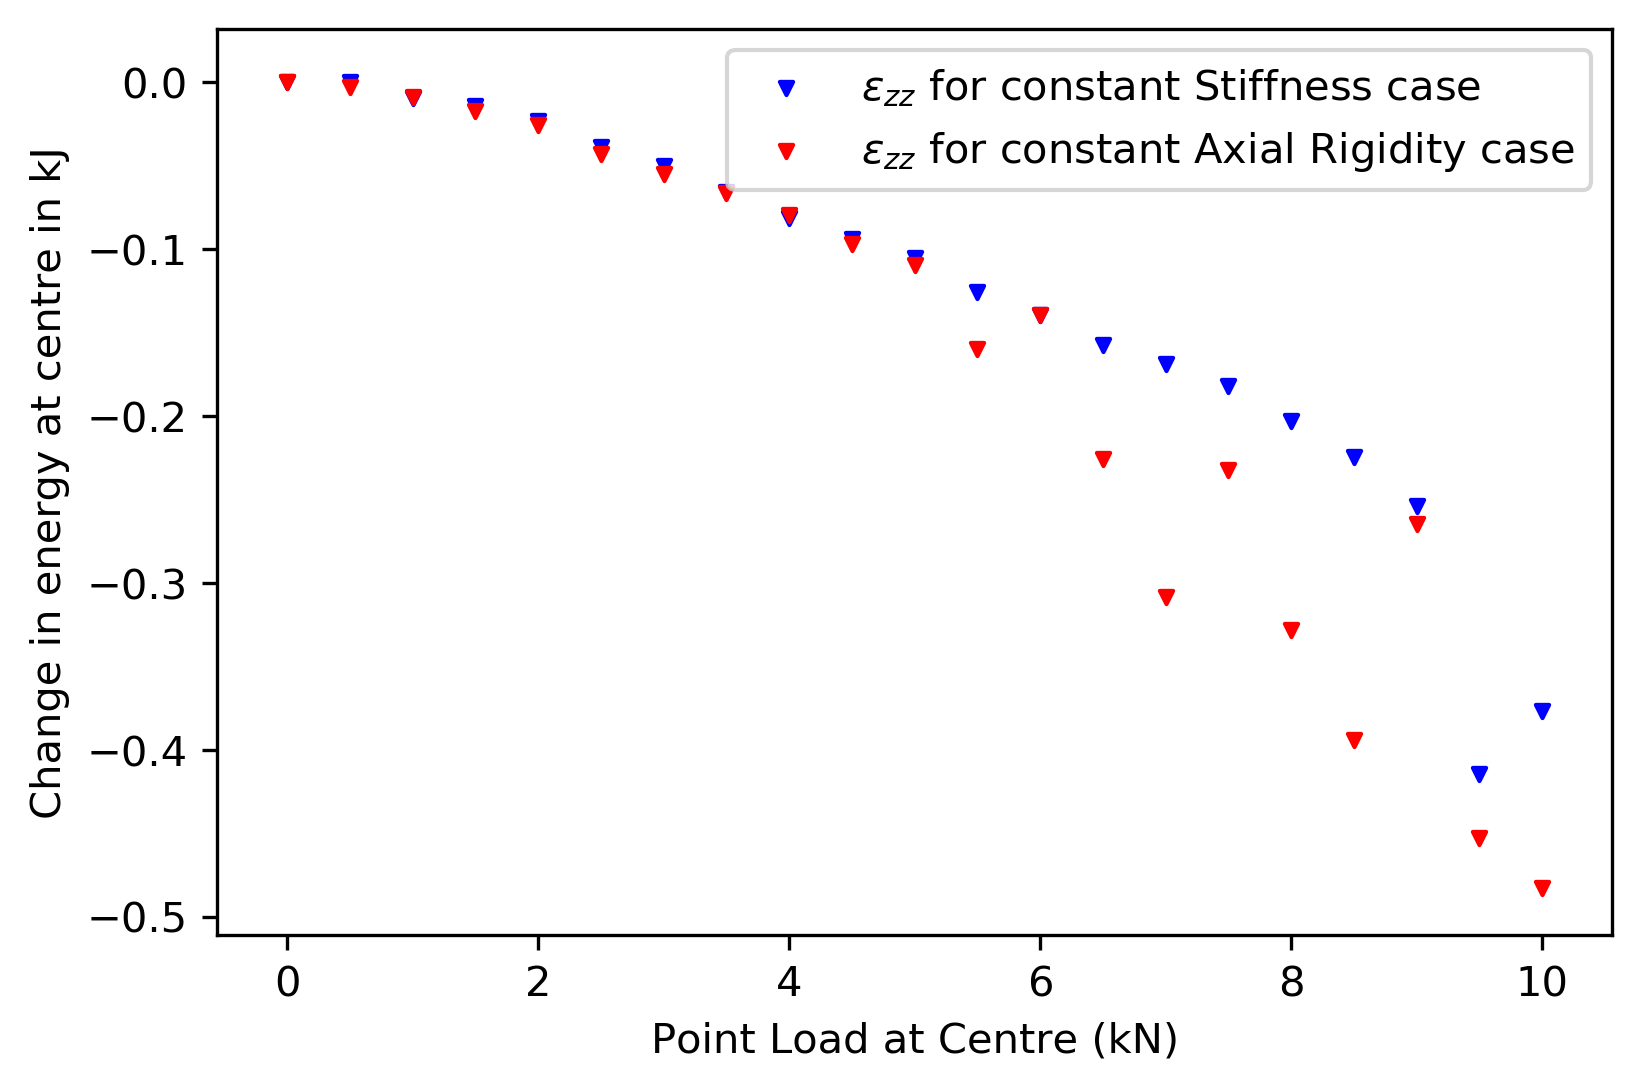
\includegraphics[width = 0.9\textwidth]{Figures/M1_c_energy.png}
    \caption{Model 1 - Type C - Change in Energy with respect to Point Load at centre}
    \label{fig:M1_c_energy}
\end{figure}

In fig~\ref{fig:M1_c_energy}, energies in the undeformed states for all forces are zero.

The energy profiles are smoother compared to the energy profiles of Type A and Type B models. The energy for Constant stiffness case at higher loading are higher than that of Constant Axial Rigidity case. Also there is a kind of oscillating pattern in the energy values obtained for Constant Axial Rigidity case for loads higher than 5 kN. 

\newpage
\subsection{Model 2}
Model 2 extends Model 1 by providing the planar layers of the Model with both in-plane bracings. Dimension of the plate is 1~m x 1~m x 0.02~m and stiffness of the springs in model are calibrated for displacement at centre for a 2 kN point load applied at centre with displacements at centre of an equivalent plate with $E = 2$ GPa and $\nu = 0.25$).

\subsubsection{Model 2 - Type A}
These models are type 2 model with 4 x 4 x 2 structure of cuboids of dimension 0.25~m x 0.25~m x 0.01~m stacked together as shown in the fig~\ref{fig:M2_a_XY} - fig~\ref{fig:M2_a_3D}.

\begin{figure}[!htbp]
\begin{minipage}{0.3\textwidth}
    \centering
    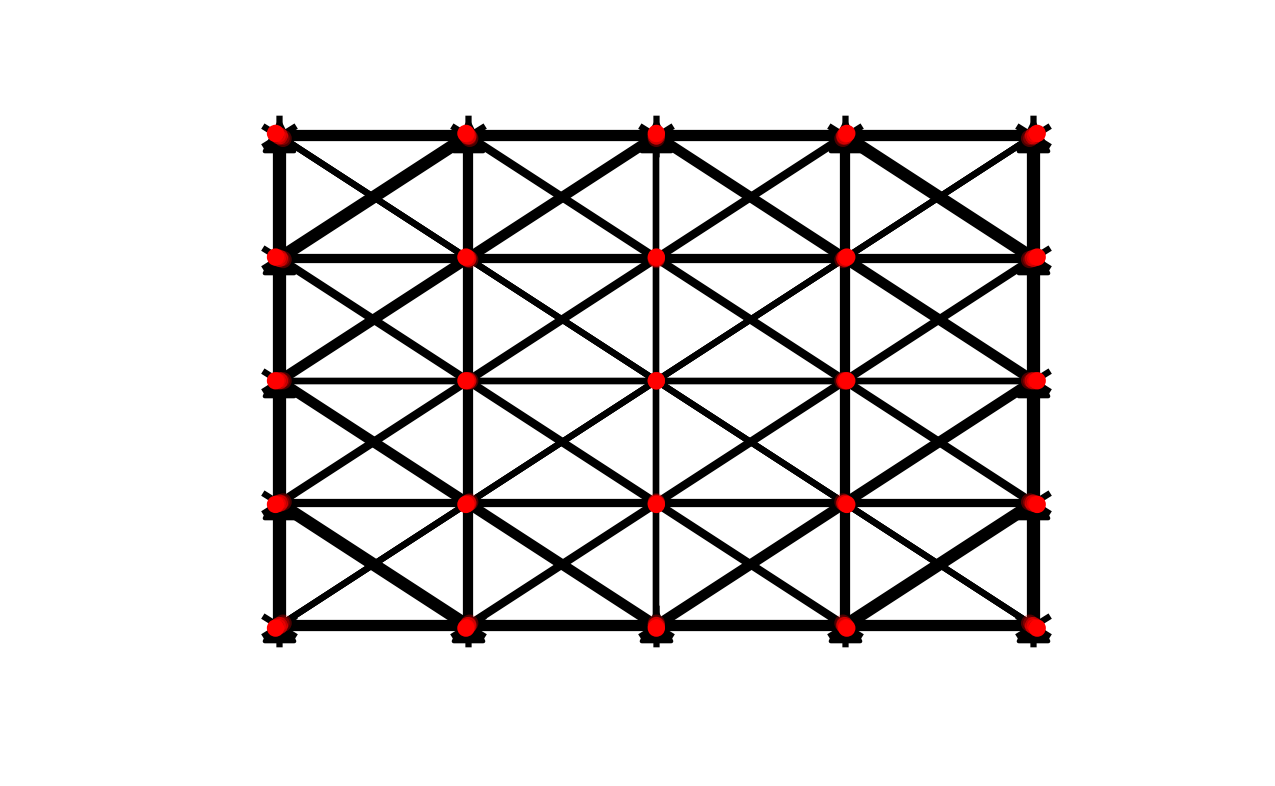
\includegraphics[width = 1\textwidth]{Figures/M2_type_a_XY.png}
    \caption{Model 2 - Type A - XY Projection}
    \label{fig:M2_a_XY}
\end{minipage}
\hspace{5mm}
\begin{minipage}{0.3\textwidth}
    \centering
    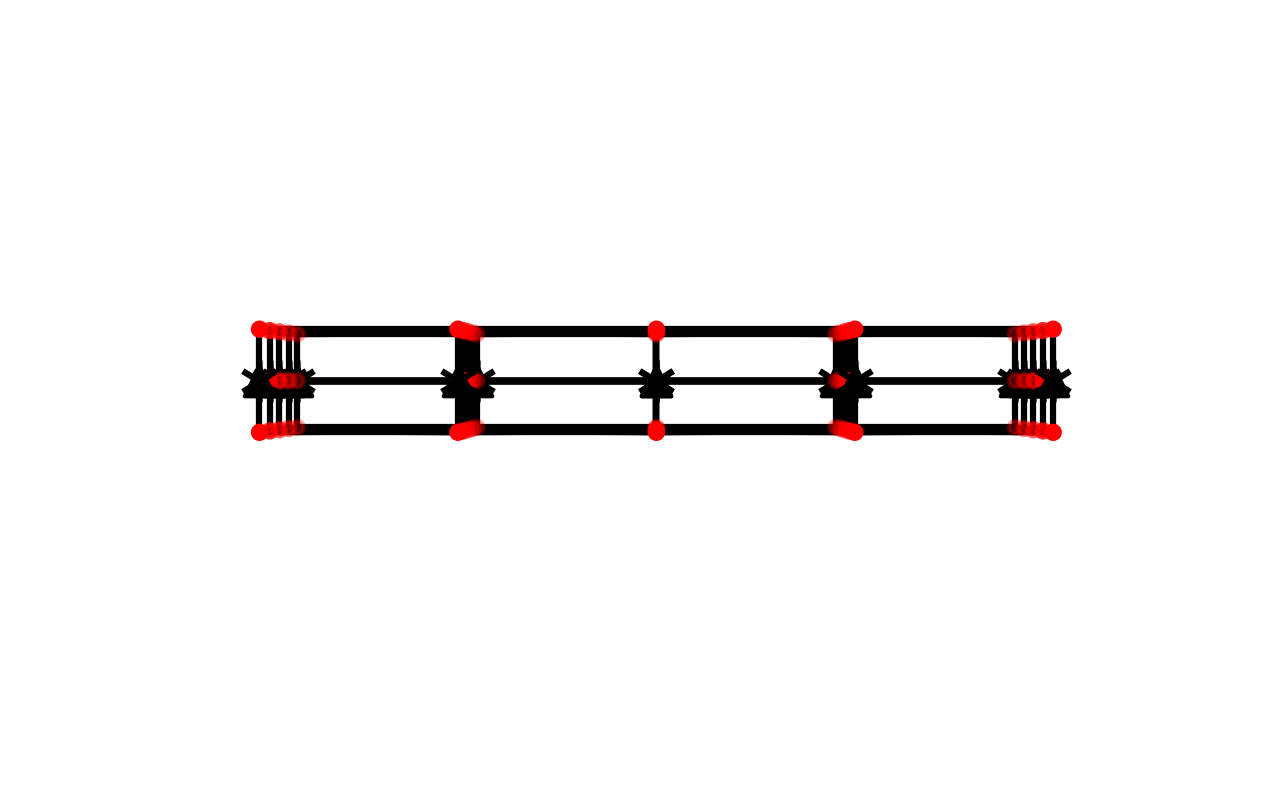
\includegraphics[width = 1\textwidth]{Figures/M2_type_a_YZ.png}
    \caption{Model 2 - Type A - YZ Projection}
    \label{fig:M2_a_YZ}
\end{minipage}
\hspace{5mm}
\begin{minipage}{0.3\textwidth}
    \centering
    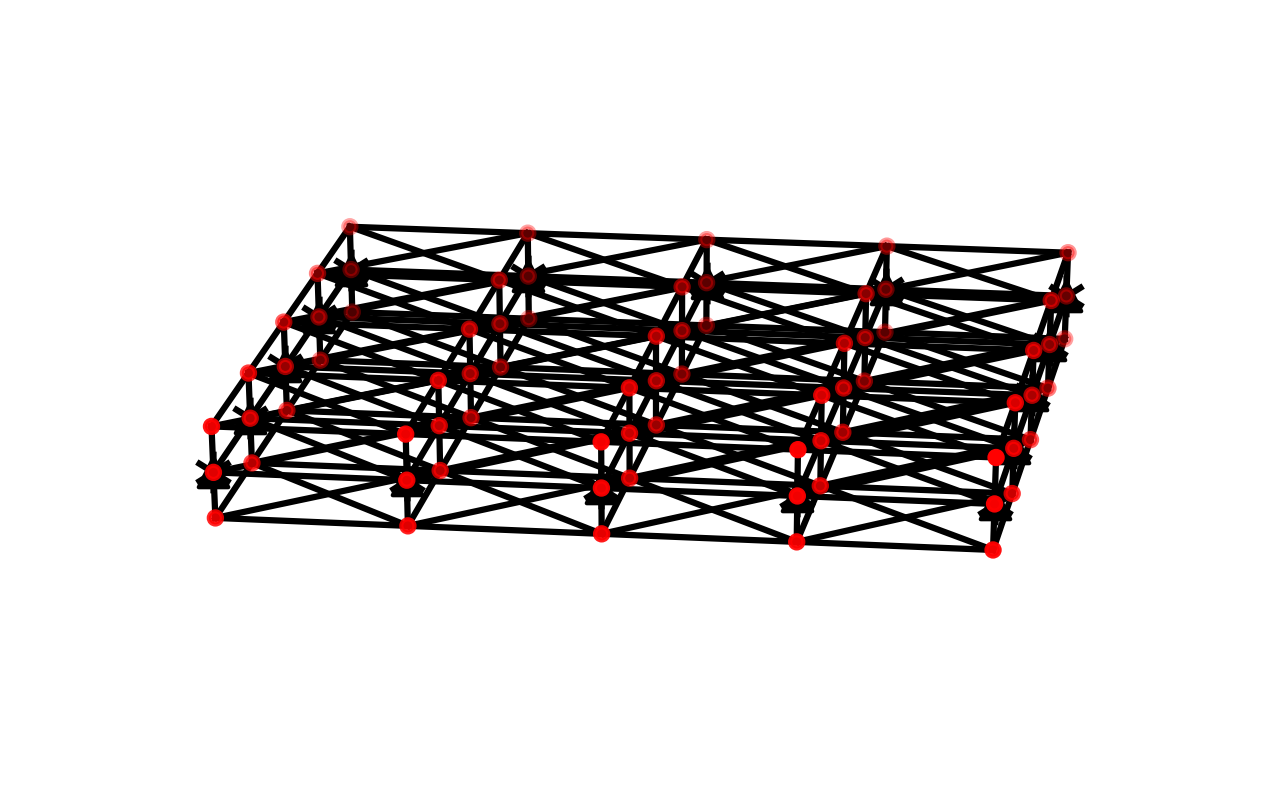
\includegraphics[width = 1\textwidth]{Figures/M2_type_a_3D.png}
    \caption{Model 2 - Type A - 3D View}
    \label{fig:M2_a_3D}
\end{minipage}
\end{figure}

The fig~\ref{fig:M2_a_plt} presents the plots for vertical deflections at centre with respect to point load applied at the centre for Constant Stiffness and Constant Axial rigidity cases.

\begin{figure}[!htbp]
    \centering
    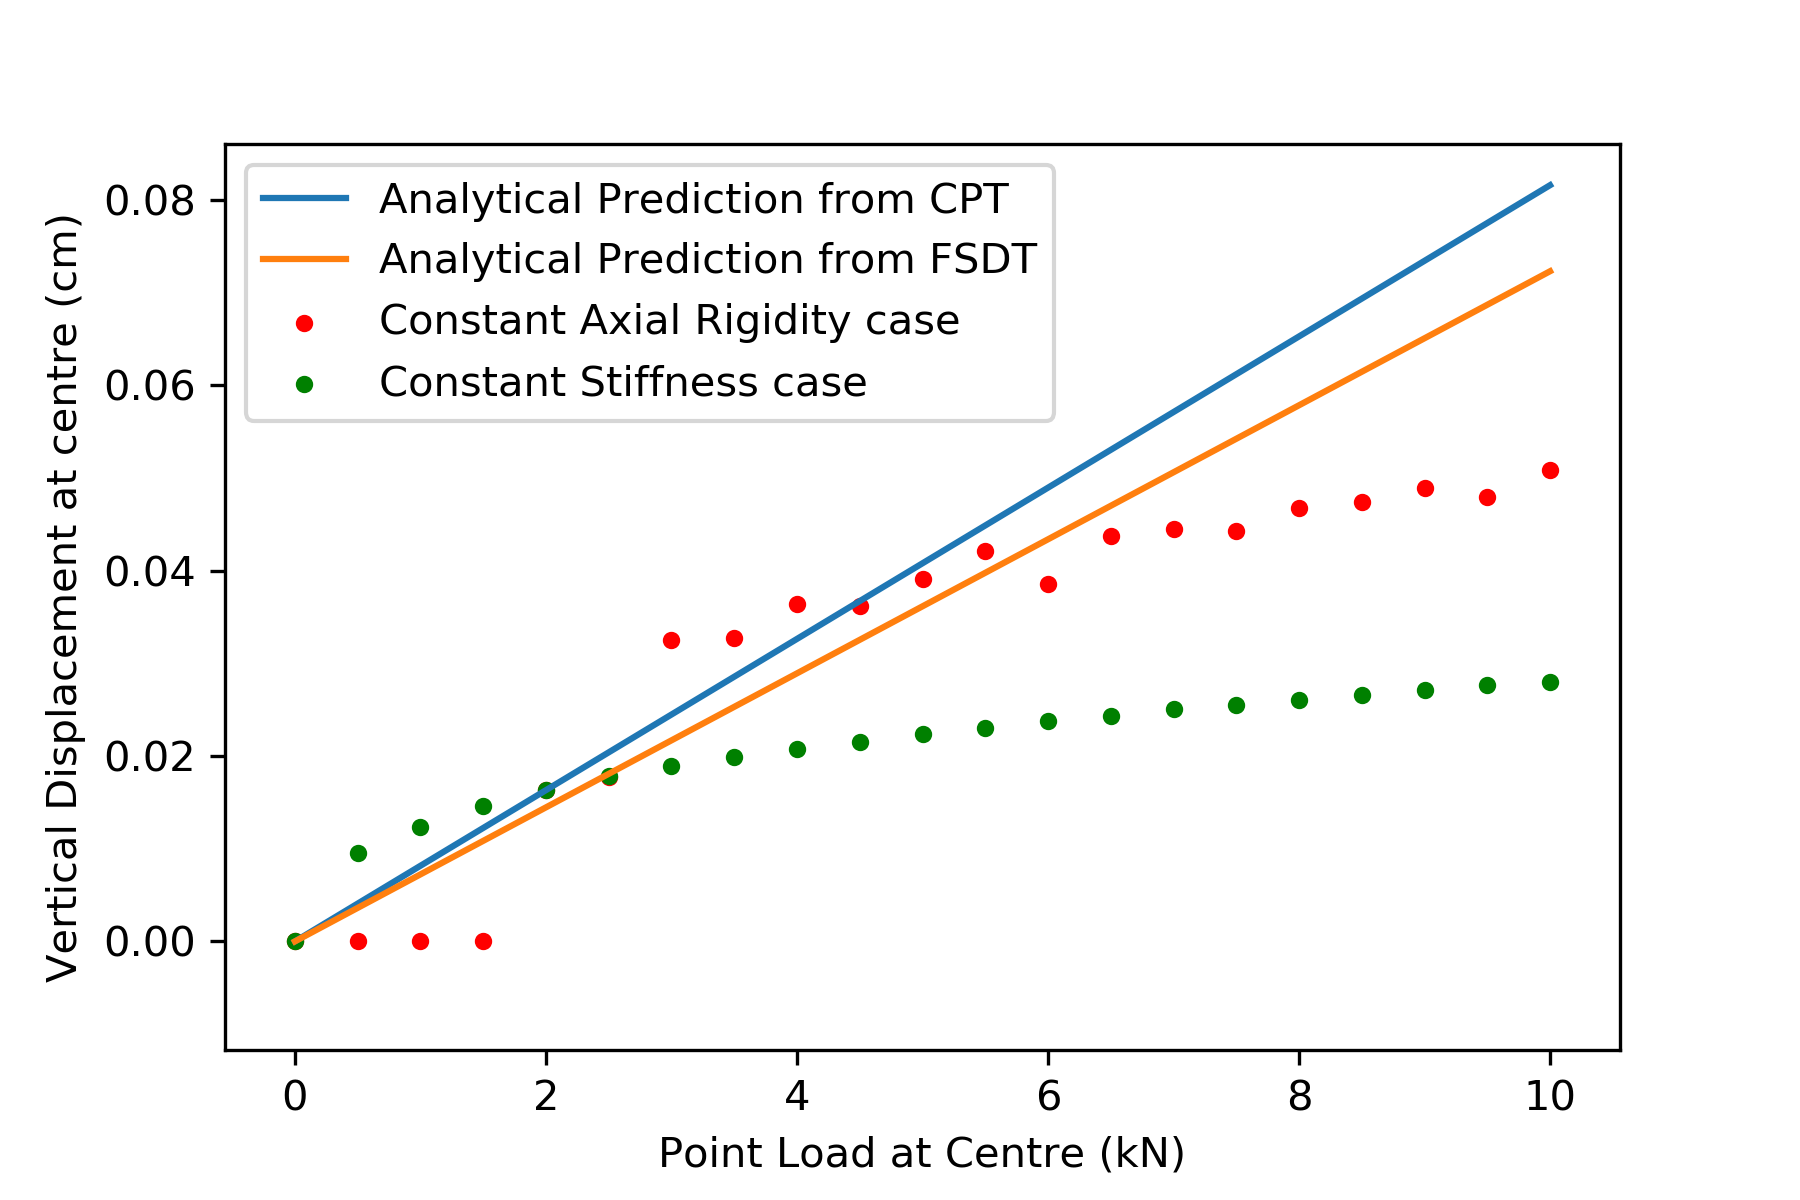
\includegraphics[width = 0.8\textwidth]{Figures/M2_a_plt.png}
    \caption{Model 2 - Type A - vertical Displacement with respect to Point Load at centre}
    \label{fig:M2_a_plt}
\end{figure}

\begin{figure}[!htbp]
    \centering
    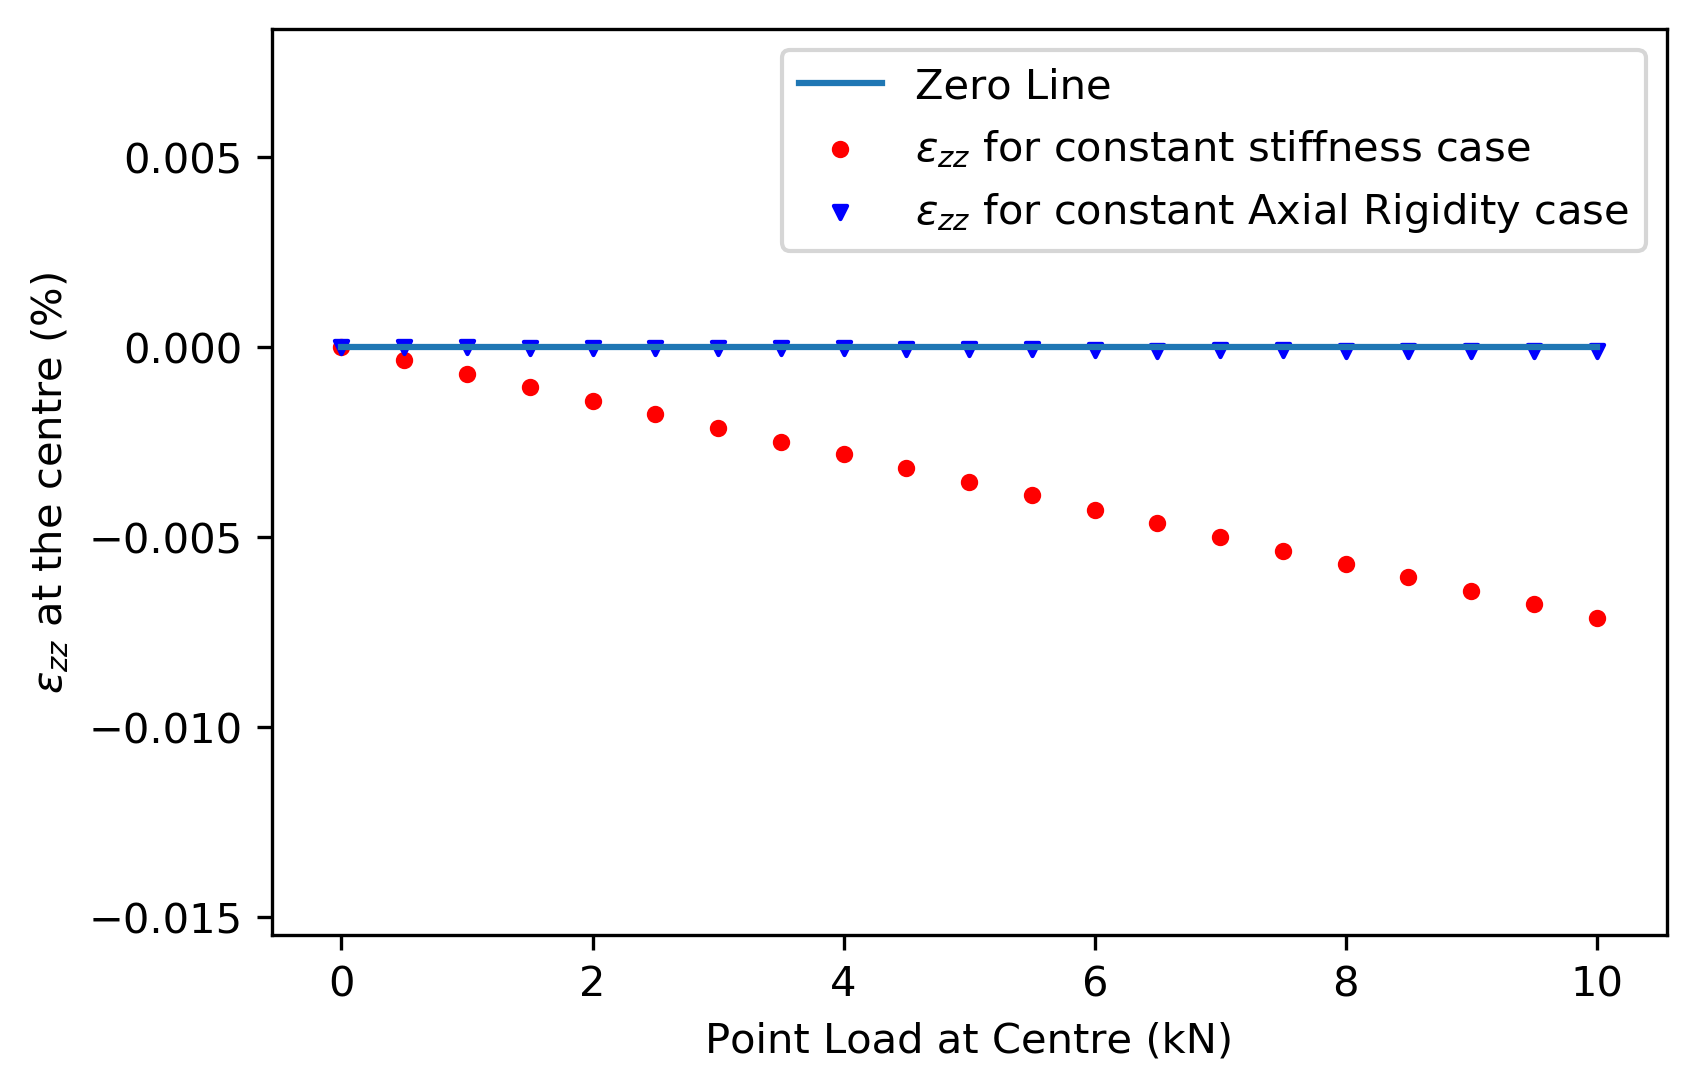
\includegraphics[width = 0.9\textwidth]{Figures/M2_a_strain.png}
    \caption{Model 2 - Type A - $\epsilon_{zz}$ with respect to Point Load at centre}
    \label{fig:M2_a_strain_plt}
\end{figure}

As evident from fig~\ref{fig:M2_a_plt}, the predictions for Constant Stiffness case, although smooth, assume a parabolic shape and achieve a plateau. They start behaving as a plate with very high stiffness at load of around 2 kN. In the case of Constant Axial Rigidity, the prediction of displacement is fragmented. Deflections at low load are zero due to ill conditioned matrices, underestimating the stiffness of plate for vertical deflection predictions then quickly rise above analytical values at a loading of around 3 kN, and finally overestimating the stiffness reaches below analytical values for higher loads. The predictions from Constant Axial Rigidity study lie closer to the analytical solution for higher loads. More close to the analytical solution from First-order Shear Deformation theory compared to Classical Plate theory.

The deviations from analytical values for Constant stiffness case can partly be explained using fig~\ref{fig:M2_a_strain_plt}. As it can be clearly seen that vertical strain is constantly increasing and the plat is being squished at the centre, this violates the assumption $\epsilon_{zz} = 0$ (eq~\ref{eq:CPT_strains_last} and eq~\ref{eq:strain_z_FSDT}). This reduces the deflection as vertical spring absorb some of the vertical deformations and as a result the Constant Stiffness study underpredicts the vertical deflection. Nonlinear behavior of the horizontal springs under action of vertical is also responsible for deviation from analytical values in two studies.

\begin{figure}[!htbp]
    \centering
    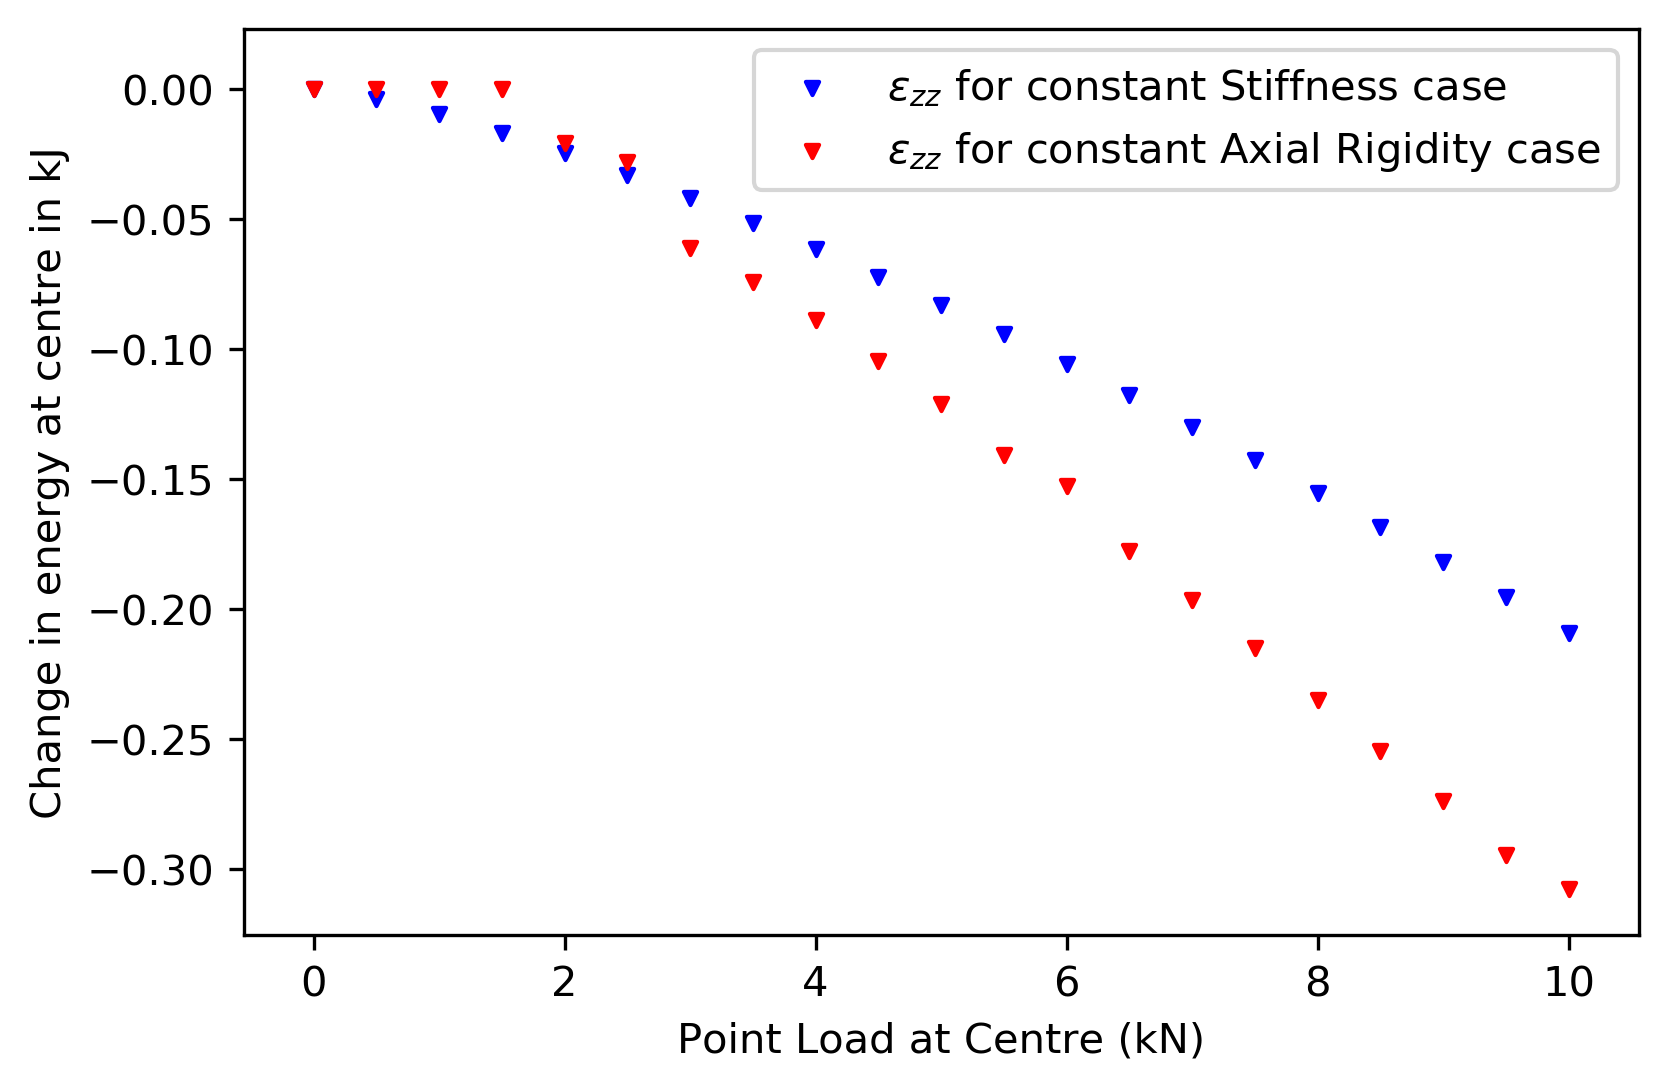
\includegraphics[width = 0.9\textwidth]{Figures/M2_a_energy.png}
    \caption{Model 2 - Type A - Change in Energy with respect to Point Load at centre}
    \label{fig:M2_a_energy}
\end{figure}

In fig~\ref{fig:M2_a_energy}, energies in the undeformed state for all forces are zero. Energy profile for Model 2 - Type A is smooth and is uniformly decreasing with force. The deflection is inversely related to the energy as it can be seen from fig~\ref{fig:M2_a_plt}. Constant Axial Rigidity model initially has higher energy than Constant stiffness case initially and as a result the deflections are lower than those predicted by Constant Stiffness Model. The energies Constant Axial Rigidity case soon drop below the energies from Constant Stiffness case and hence the deflection predicted by Axial Rigidity case are higher than Constant Stiffness case.

\subsubsection{Model 2 - Type B}
Model 2 - Type B is 10 x 10 x 2 structure of Model 2 cuboids of dimensions 0.1~m x 0.1~m x 0.01~m. The model is shown in fig~\ref{fig:M2_b_XY} - fig~\ref{fig:M2_b_3D}

\begin{figure}[!htbp]
\begin{minipage}{0.3\textwidth}
    \centering
    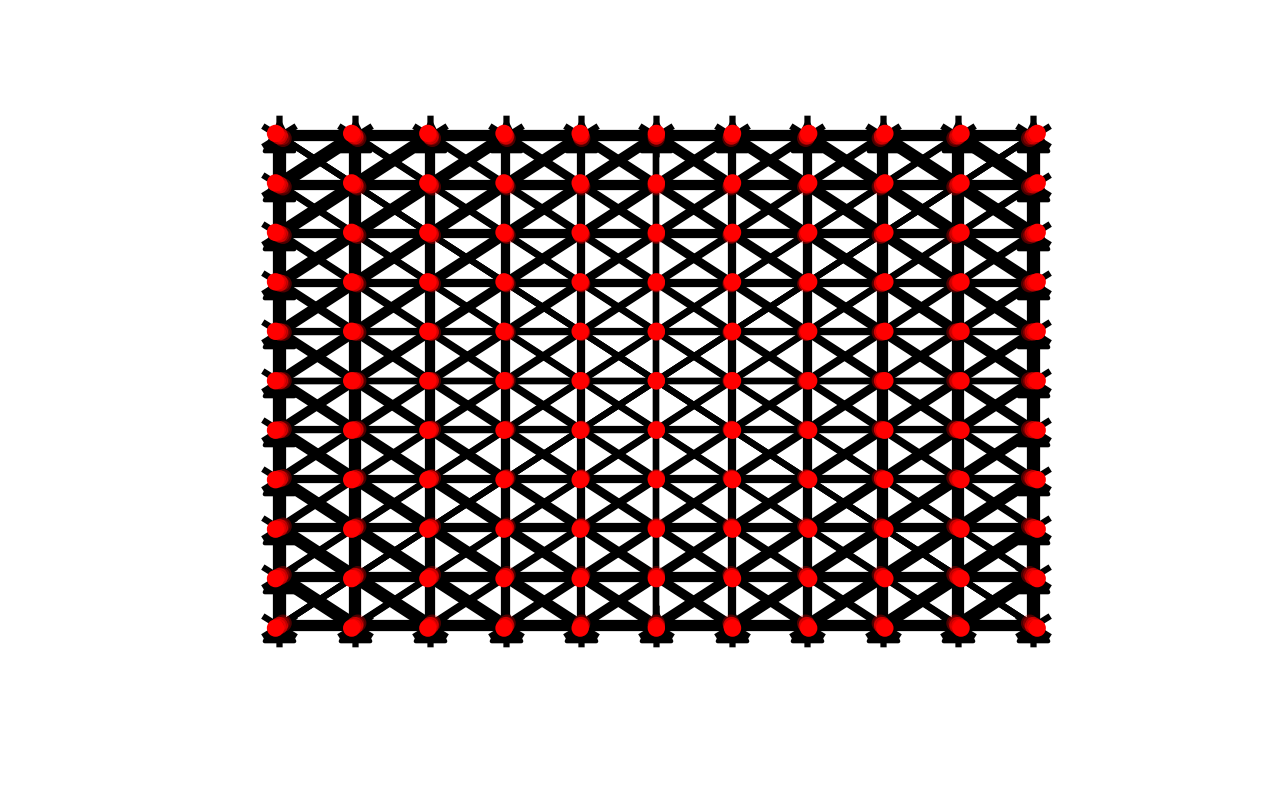
\includegraphics[width = 1\textwidth]{Figures/M2_b_XY.png}
    \caption{Model 2 - Type B - XY Projection}
    \label{fig:M2_b_XY}
\end{minipage}
\hspace{5mm}
\begin{minipage}{0.3\textwidth}
    \centering
    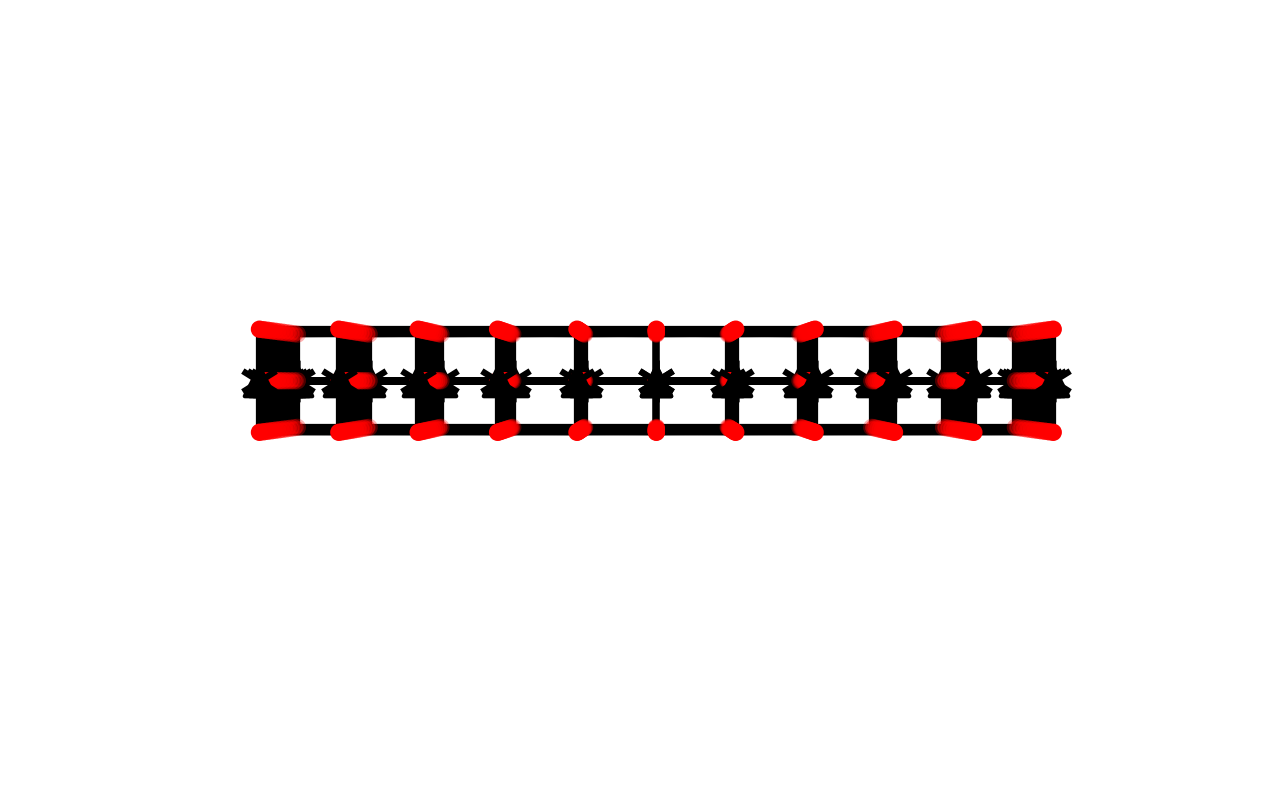
\includegraphics[width = 1\textwidth]{Figures/M2_b_YZ.png}
    \caption{Model 2 - Type B - YZ Projection}
    \label{fig:M2_b_YZ}
\end{minipage}
\hspace{5mm}
\begin{minipage}{0.3\textwidth}
    \centering
    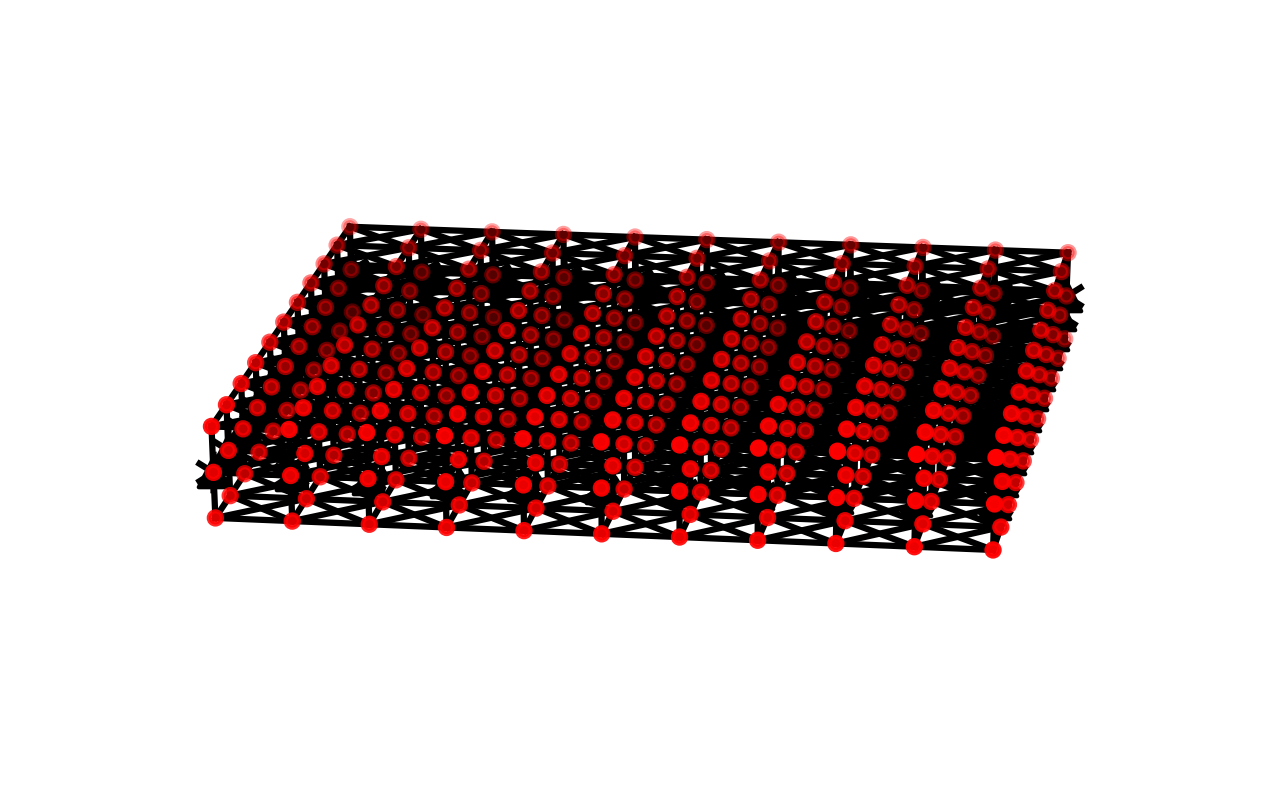
\includegraphics[width = 1\textwidth]{Figures/M2_b_3D.png}
    \caption{Model 2 - Type B - 3D View}
    \label{fig:M2_b_3D}
\end{minipage}
\end{figure}

The plots corresponding to Model 2 - Type B are shown in fig~\ref{fig:M2_b_plt} - fig~\ref{fig:M2_b_energy}. The deflection predictions for Constant Stiffness case assumes a parabolic shape similar to that in Model 2 - Type A. However, in Type B model, the predictions from Constant Axial Rigidity model closely follow the predictions from Constant Stiffness model, although this results in larger deviation from analytical results. The deviation of the prediction can again be explained through the combination of violation of the assumption $\epsilon_{zz} = 0$ and non-linear behavior of horizontal spring system under vertical loading as discussed in Model 2 - Type A section. The inverse relation between energy and deflection discussed in Model 2 - Type A section also holds.

\begin{figure}[!htbp]
    \centering
    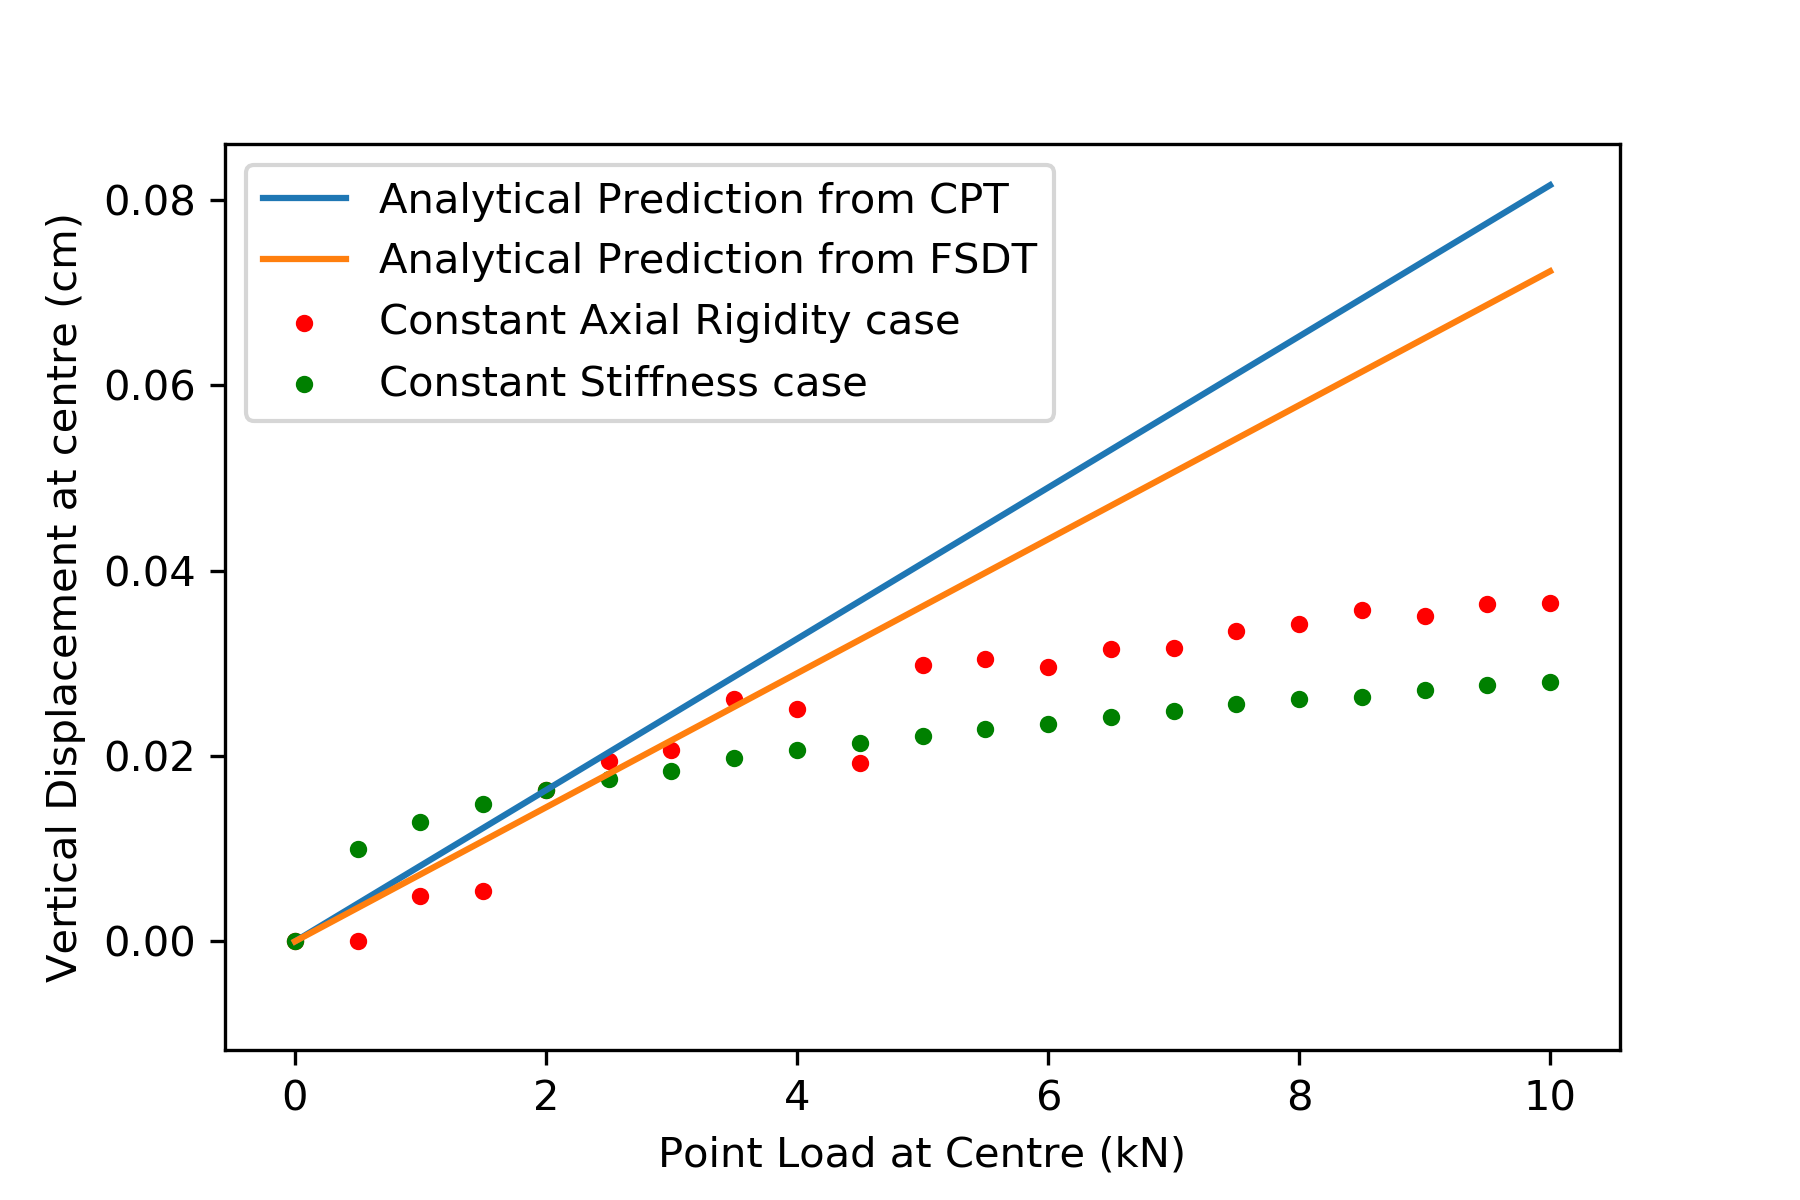
\includegraphics[width = 0.8\textwidth]{Figures/M2_b_plt.png}
    \caption{Model 2 - Type B - vertical Displacement with respect to Point Load at centre}
    \label{fig:M2_b_plt}
\end{figure}

\begin{figure}[!htbp]
    \centering
    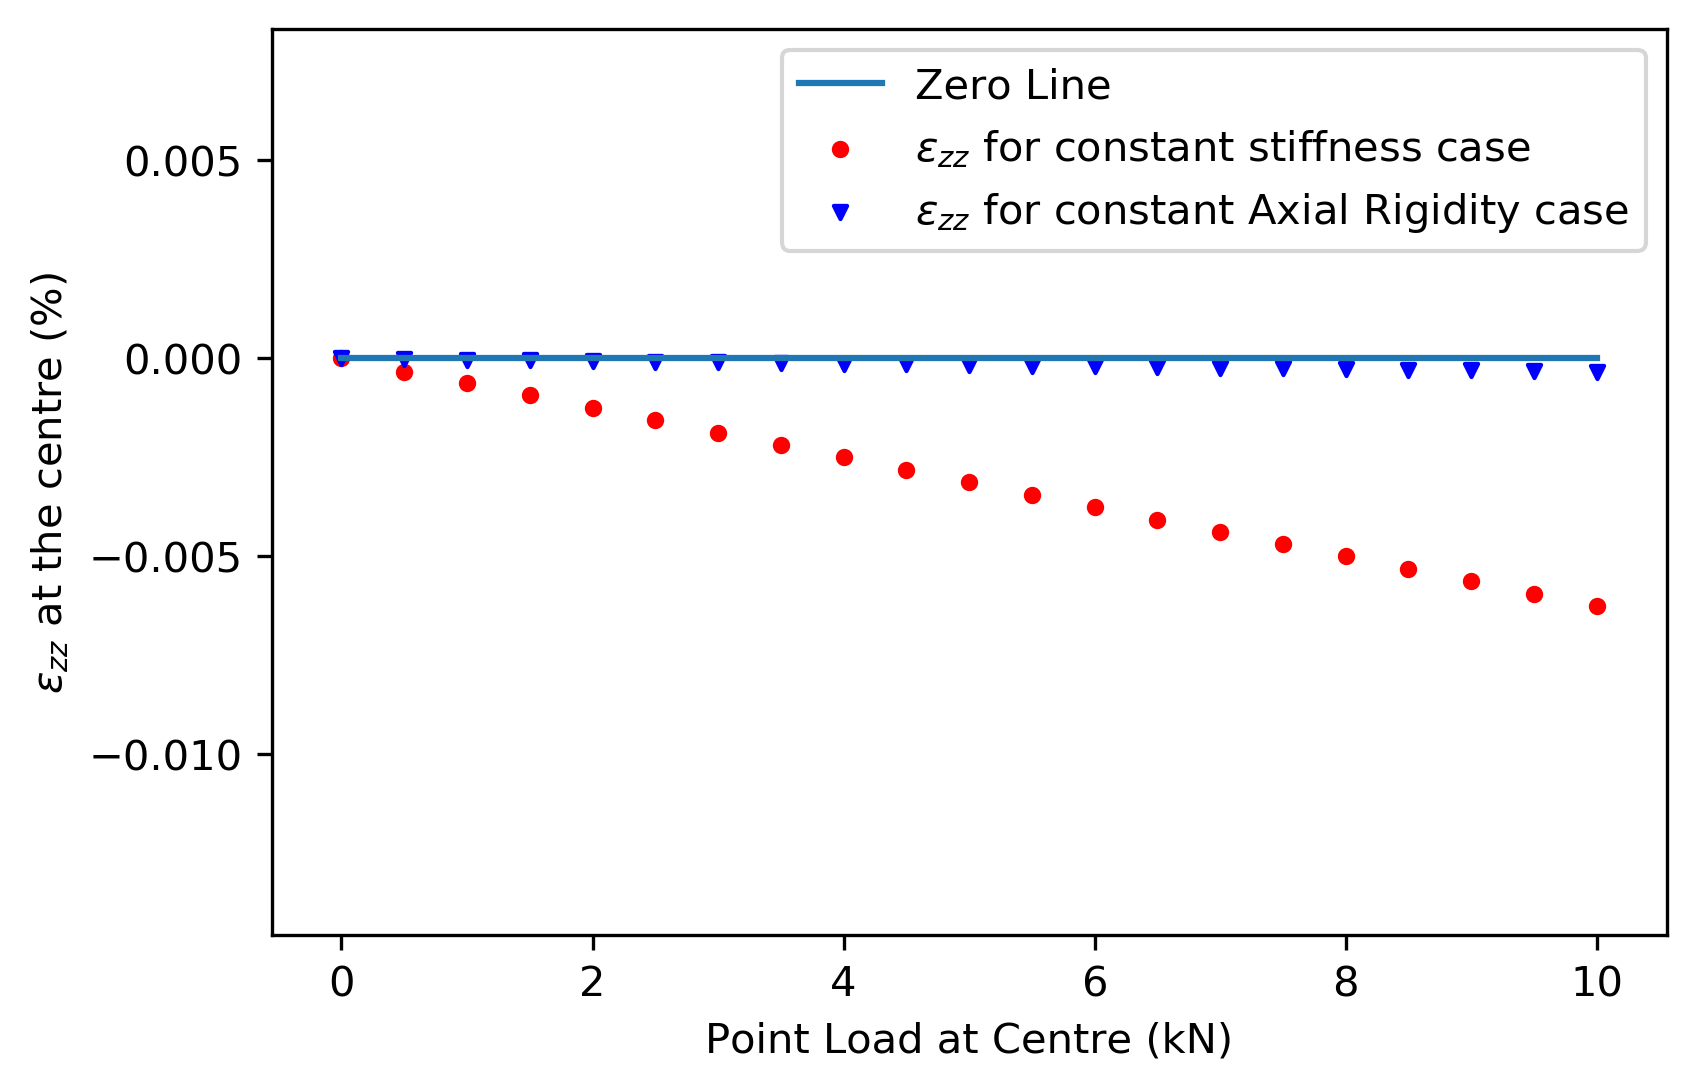
\includegraphics[width = 0.9\textwidth]{Figures/M2_b_strain.png}
    \caption{Model 2 - Type B - $\epsilon_{zz}$ with respect to Point Load at centre}
    \label{fig:M2_b_strain_plt}
\end{figure}


\begin{figure}[!htbp]
    \centering
    \includegraphics[width = 0.9\textwidth]{Figures/M2_b_energy.png}
    \caption{Model 2 - Type B - Change in Energy with respect to Point Load at centre}
    \label{fig:M2_b_energy}
\end{figure}

 \newpage
 \subsubsection{Model 2 - Type C}
 Model 2 - Type C is 20 x 20 x 2 structure of Model 2 cuboids of dimensions 0.05~m x 0.05~m x 0.01~m. The model is shown in fig~\ref{fig:M2_c_XY} - fig~\ref{fig:M2_c_3D}

\begin{figure}[!htbp]
\begin{minipage}{0.3\textwidth}
    \centering
    \includegraphics[width = 1\textwidth]{Figures/M2_type_c_XY.png}
    \caption{Model 2 - Type C - XY Projection}
    \label{fig:M2_c_XY}
\end{minipage}
\hspace{5mm}
\begin{minipage}{0.3\textwidth}
    \centering
    \includegraphics[width = 1\textwidth]{Figures/M2_type_c_YZ.png}
    \caption{Model 2 - Type C - YZ Projection}
    \label{fig:M2_c_YZ}
\end{minipage}
\hspace{5mm}
\begin{minipage}{0.3\textwidth}
    \centering
    \includegraphics[width = 1\textwidth]{Figures/M2_type_c_3D.png}
    \caption{Model 2 - Type C - 3D View}
    \label{fig:M2_c_3D}
\end{minipage}
\end{figure}

The plots corresponding to Model 2 - Type C are shown in fig~\ref{fig:M2_c_plt} - fig~\ref{fig:M2_c_energy}. For Model 2 Type C case, both, Constant Stiffness and Constant Axial Rigidity study, predict smooth deflection curve and closely resemble each other. However, they both underpredict the deflection compared to those obtained using analytical solutions. 

\begin{figure}[!htbp]
    \centering
    \includegraphics[width = 0.8\textwidth]{Figures/M2_c_plt.png}
    \caption{Model 2 - Type C - vertical Displacement with respect to Point Load at centre}
    \label{fig:M2_c_plt}
\end{figure}

\begin{figure}[!htbp]
    \centering
    \includegraphics[width = 0.9\textwidth]{Figures/M2_c_strain.png}
    \caption{Model 2 - Type C - $\epsilon_{zz}$ with respect to Point Load at centre}
    \label{fig:M2_c_strain_plt}
\end{figure}

\begin{figure}[!htbp]
    \centering
    \includegraphics[width = 0.9\textwidth]{Figures/M2_c_energy.png}
    \caption{Model 2 - Type C - Change in Energy with respect to Point Load at centre}
    \label{fig:M2_c_energy}
\end{figure}

Strain for the Model 2 - Type C case are constantly increasing with the applied load as evident from fig~\ref{fig:M2_c_strain_plt}. Strain for the Constant Axial Rigidity case are lower than those of Constant Stiffness case but both of them violate the assumption that $\epsilon_{zz} = 0$ (eq~\ref{eq:CPT_strains_last} and eq~\ref{eq:strain_z_FSDT}). This coupled with non-linear behavior of horizontal spring system under vertical loading result in underestimation of vertical deflections by the model compared to those predicted by analytical theories. The energy profile predicted by the model is also smooth as compared to Model 2 - Type A and Model 2 - Type B indicating that model is numerically stable and matrices involved have low condition number and are well conditioned.

\newpage
\subsection{Model 3}
Model 3 comprises of cuboidal unit cells with in-plane diagonals on top and bottom plane and all body diagonals. Dimension of the plate is 1~m x 1~m x 0.02~m and stiffness of the springs in model are calibrated for displacement at centre for a 2 kN point load applied at centre with displacements at centre of an equivalent plate with $E = 2$ GPa and $\nu = 0.25$).

\subsubsection{Model 3 - Type A}
These models are type 3 model with 4 x 4 x 2 structure of cuboids of dimension 0.25~m x 0.25~m x 0.01~m stacked together as shown in the fig~\ref{fig:M3_a_XY} - fig~\ref{fig:M3_a_3D}.

\begin{figure}[!htbp]
\begin{minipage}{0.3\textwidth}
    \centering
    \includegraphics[width = 1\textwidth]{Figures/M3_type_a_XY.png}
    \caption{Model 3 - Type A - XY Projection}
    \label{fig:M3_a_XY}
\end{minipage}
\hspace{5mm}
\begin{minipage}{0.3\textwidth}
    \centering
    \includegraphics[width = 1\textwidth]{Figures/M3_type_a_YZ.png}
    \caption{Model 3 - Type A - YZ Projection}
    \label{fig:M3_a_YZ}
\end{minipage}
\hspace{5mm}
\begin{minipage}{0.3\textwidth}
    \centering
    \includegraphics[width = 1\textwidth]{Figures/M3_type_a_3D.png}
    \caption{Model 3 - Type A - 3D View}
    \label{fig:M3_a_3D}
\end{minipage}
\end{figure}

The fig~\ref{fig:M3_a_plt} presents the plots for vertical deflections at centre with respect to point load applied at the centre for Constant Stiffness and Constant Axial rigidity cases. The model predicts very similar deflection for two cases which lies closer to the predictions from the First-order Shear Deformation theory compared to the Classical Plate theory, however these predictions deviate significantly from the analytical predictions. The underestimation of deflection like previous cases can be attribute to non-linear response of horizontal spring system under vertical load. However, one peculiar point to notice is that in fig~\ref{fig:M3_a_strain_plt}, even though the vertical strain for Constant axial rigidity case and Constant stiffness case differ significantly, the vertical deflection at centre predicted by the two at centre are almost equal. Also, for loading of 9 kN under Constant Axial Rigidity case, model is crushed at centre (fig~\ref{fig:M3_a_crushed}) resulting in very high strains. This anomaly might be due to some numerical instability leading to an ill conditioned matrix and hence the irregular strain.

\begin{figure}[!htbp]
    \centering
    \includegraphics[width = 0.8\textwidth]{Figures/M3_a_plt.png}
    \caption{Model 3 - Type A - vertical Displacement with respect to Point Load at centre}
    \label{fig:M3_a_plt}
\end{figure}

\begin{figure}[!htbp]
    \centering
    \includegraphics[width = 0.9\textwidth]{Figures/M3_a_strain.png}
    \caption{Model 3 - Type A - $\epsilon_{zz}$ with respect to Point Load at centre}
    \label{fig:M3_a_strain_plt}
\end{figure}

\begin{figure}
    \centering
    \includegraphics{Figures/M3_a_crushed.png}
    \caption{Model 3 - Type A - Crushed vertical springs under loading of 9 kN resulting in very high $\epsilon_{zz}$}
    \label{fig:M3_a_crushed}
\end{figure}

In fig~\ref{fig:M3_a_energy}, energies in the undeformed state for all forces are zero. Energy profile for Model 3 - Type A is smooth, uniformly decreasing with force, and is almost equal for the case of Constant Axial Rigidity and Constant Stiffness. One anamoly present at the load of 9 kN, as explained earlier, is most probably due to some numerical instability.

\begin{figure}[!htbp]
    \centering
    \includegraphics[width = 0.9\textwidth]{Figures/M3_a_energy.png}
    \caption{Model 3 - Type A - Change in Energy with respect to Point Load at centre}
    \label{fig:M3_a_energy}
\end{figure}

\subsubsection{Model 3 - Type B}
Model 3 - Type B is 10 x 10 x 2 structure of Model 2 cuboids of dimensions 0.1~m x 0.1~m x 0.01~m. The model is shown in fig~\ref{fig:M3_b_XY} - fig~\ref{fig:M3_b_3D}

\begin{figure}[!htbp]
\begin{minipage}{0.3\textwidth}
    \centering
    \includegraphics[width = 1\textwidth]{Figures/M3_b_XY.png}
    \caption{Model 3 - Type B - XY Projection}
    \label{fig:M3_b_XY}
\end{minipage}
\hspace{5mm}
\begin{minipage}{0.3\textwidth}
    \centering
    \includegraphics[width = 1\textwidth]{Figures/M3_b_YZ.png}
    \caption{Model 3 - Type B - YZ Projection}
    \label{fig:M3_b_YZ}
\end{minipage}
\hspace{5mm}
\begin{minipage}{0.3\textwidth}
    \centering
    \includegraphics[width = 1\textwidth]{Figures/M3_b_3D.png}
    \caption{Model 3 - Type B - 3D View}
    \label{fig:M3_b_3D}
\end{minipage}
\end{figure}

The plots corresponding to Model 3 - Type B are shown in fig~\ref{fig:M3_b_plt} - fig~\ref{fig:M3_b_energy}. The deflection predictions for Constant Stiffness case and Constant Axial Rigidity case are almost equal and assume a parabolic shape similar to that in Model 3 - Type A. However, the strains for this case are considerably higher than those of Model 3 - Type A despite the vertical deflection at centre being almost same. Also, the vertical strain corresponding to the Constant Axial Rigidity cases are much lower than those of Constant Stiffness case.

\begin{figure}[!htbp]
    \centering
    \includegraphics[width = 0.8\textwidth]{Figures/M3_b_plt.png}
    \caption{Model 3 - Type B - vertical Displacement with respect to Point Load at centre}
    \label{fig:M3_b_plt}
\end{figure}

\begin{figure}[!htbp]
    \centering
    \includegraphics[width = 0.9\textwidth]{Figures/M3_b_strain.png}
    \caption{Model 3 - Type B - $\epsilon_{zz}$ with respect to Point Load at centre}
    \label{fig:M3_b_strain_plt}
\end{figure}

The energy profile as shown in the fig~\ref{fig:M3_b_energy} is almost same as that of Model 3 - Type A (fig~\ref{fig:M3_a_energy}), except for the anomaly in Model 3- Type A profile at 9 kN load. 

\begin{figure}[!htbp]
    \centering
    \includegraphics[width = 0.9\textwidth]{Figures/M3_b_energy.png}
    \caption{Model 3 - Type B - Change in Energy with respect to Point Load at centre}
    \label{fig:M3_b_energy}
\end{figure}

 \newpage
 \subsubsection{Model 3 - Type C}
 Model 3 - Type C is 20 x 20 x 2 structure of Model 3 cuboids of dimensions 0.05~m x 0.05~m x 0.01~m. The model is shown in fig~\ref{fig:M3_c_XY} - fig~\ref{fig:M3_c_3D}

\begin{figure}[!htbp]
\begin{minipage}{0.3\textwidth}
    \centering
    \includegraphics[width = 1\textwidth]{Figures/M3_type_c_XY.png}
    \caption{Model 3 - Type C - XY Projection}
    \label{fig:M3_c_XY}
\end{minipage}
\hspace{5mm}
\begin{minipage}{0.3\textwidth}
    \centering
    \includegraphics[width = 1\textwidth]{Figures/M3_type_c_YZ.png}
    \caption{Model 3 - Type C - YZ Projection}
    \label{fig:M3_c_YZ}
\end{minipage}
\hspace{5mm}
\begin{minipage}{0.3\textwidth}
    \centering
    \includegraphics[width = 1\textwidth]{Figures/M3_type_c_3D.png}
    \caption{Model 3 - Type C - 3D View}
    \label{fig:M3_c_3D}
\end{minipage}
\end{figure}

The plots corresponding to Model 3 - Type C are shown in fig~\ref{fig:M3_c_plt} - fig~\ref{fig:M3_c_energy}. This model predicts deflection accurately in accordance with the First-order Shear Deformation theory and lies very close to Classical plate theory. In this model, both, Constant Axial Rigidity case and Constant Stiffness case predict the deflections accurately as can be seen from fig~\ref{fig:M3_c_plt}. The Constant Axial Rigidity case has much lower strain than constant Stiffness case, however in both the case, vertical strains are much smaller than those of Model 3 - Type A and Model 3 - Type B.

\begin{figure}[!htbp]
    \centering
    \includegraphics[width = 0.8\textwidth]{Figures/M3_c_plt.png}
    \caption{Model 3 - Type C - vertical Displacement with respect to Point Load at centre}
    \label{fig:M3_c_plt}
\end{figure}

\begin{figure}[!htbp]
    \centering
    \includegraphics[width = 0.9\textwidth]{Figures/M3_c_strain.png}
    \caption{Model 3 - Type C - $\epsilon_{zz}$ with respect to Point Load at centre}
    \label{fig:M3_c_strain_plt}
\end{figure}

As evident from the scale of Y-Axis of fig~\ref{fig:M3_c_energy}, the decrease in energy in Model C - Type 3 study is much smaller than other models and cases. Here as well, the Constant Axial Rigidity case and Constant Stiffness case, follow each other very closely.

\begin{figure}[!htbp]
    \centering
    \includegraphics[width = 0.9\textwidth]{Figures/M3_c_energy.png}
    \caption{Model 3 - Type C - Change in Energy with respect to Point Load at centre}
    \label{fig:M3_c_energy}
\end{figure}

\newpage
\section{Conclusion}

Based on the studies above, following conclusions can be drawn:
\begin{enumerate}
    \item It is observed that vertical deflections predicted by Constant Axial Stiffness case are generally higher and closer to analytical solutions as compared to those predicted by Constant Stiffness case. Also, the vertical normal strains in model under the Constant Axial Rigidity strain are closer to zero as compared to the Constant Stiffness case. This justifies the importance of the assumption that $\epsilon_{zz} = 0$ in the results of analytical solution and how squeezing of plate under the concentrated vertical loading leads to lowering of vertical deflection at the centre of the plate.
    \item The magnitude of energy change is generally higher for the Constant Axial Rigidity case compared to Constant Axial Rigidity case. This result can be attributed to the higher displacements that the vertically applied force undergoes under Constant Axial Rigidity case. For higher deflection, springs are stretched more and this tends to increase the energy system but it is overcompensated by the work of vertical springs leading to equilibrium at higher displacement as opposed to the Constant Stiffness case.
    \item It can be observed that increasing the number of nodes and springs (or equivalently breaking the plate into more number of cells), i.e. moving from Type A system to Type C systems, the displacement profiles become more regular and the predictions from the Constant Stiffness case and Constant Axial Rigidity case come closer to each other. Also adding in-plane diagonals and body diagonals, i.e. moving from Model 1 to Model 3, has a effect of regularizing and taking predictions closer to the analytical solutions, especially when going from Model 2 to Model 3. This increase in accuracy of the model might be due to bending stiffness that is added to model by using body diagonals. Model 1 and Model 2 do not have any direct connection between two layers and vertical springs provide second order reaction forces for small displacement between planes.
    \item The strains in vertical direction ($\epsilon_{zz}$) are generally higher for Constant Stiffness case than Constant Axial rigidity case. As the number of node and springs are increased, i.e. as we move from Type A to Type C models, vertical strain increases (except in case of Model 3 where vertical strain decreases on moving from Type B to Type C). Moreover, strains increase on moving from Model 1 to Model 3 as the diagonal springs are added. Also, Moving from Type A models to Type C models, the cases in which vertical strains are very high increase. All this indicates that at times it is energetically, at least locally, more favourable to crush the vertical springs in the centre rather than distributing the energy between springs of the horizontal layers.
    \item It is observed that out of Type A, Type B, and Type C Models, Type B has the highest discrepancy between strains predicted by Constant Stiffness and Constant Axial rigidity case. Also Type B models, although marginally, have less regularity compared to Type A and Type C. This indicated some kind of numerical instability in between at Type B Models as we move from Type A models to Type C Models.
    \item The energy profile for Models of all type are mostly uniform and have a predictable pattern. The difference between energy predictions for a given loading by Constant Axial Rigidity case and Constant Stiffness Case appears to increase as one moves from Type A models to Type C models. In most of the cases, the increased discrepancy is due to changes in energies change predicted by Constant Axial Rigidity case while the energy change prediction for Constant Stiffness case remains almost same among models for a given load.
    \item Interestingly, time taken by the program to minimize the energy for model is less than the time taken for minimizing the energy of model 2 despite the increased number of springs. This suggests presence of some kind of numerical stability in type 3 models compare to type 2 models.
    \item While most of the models agree with analytical solution at low loads, they deviate significantly from the analytical solution at higher loads. Model 3 - Type C which provides the deflection results matching very well at all loads has few peculiar properties which are highlighted below.
    \begin{enumerate}
        \item Magnitude of energy change in model 3 - Type C under any given load is much smaller than energy changes in all the other Type and Model despite the fact that the displacements predicted by Model 3 - Type C predicts higher deflections at the centre. This means that although the vertical load does more work, it is compensated by the energy developed in the springs and hence the system has much lower energy change compared to other types and models.
        \item Even though the strains are higher than some of the other cases and differ significantly for Constant Strain and Constant Axial Rigidity case, the energies predicted under any given vertical loading are small compared to other type and models and very close to each other for two cases.
    \end{enumerate}
\end{enumerate}

\section{Limitations of Model and Suggested Improvements}
Following this study, few short comings of the models and possible ways to remedy the situation are pointed out in the following points.
\begin{enumerate}
    \item We can the violation of the assumption $\epsilon_{zz} = 0$ for almost all the models. In some cases the vertical springs are crushed resulting in strains higher than 50\% and are source of errors and deviation from the analytical results. There are two ways in which this problem can be tackled:
    \begin{enumerate}
        \item Providing the vertical springs with stiffness orders of magnitude higher than the horizontal springs. This provides more flexibility to vary vary vertical spring stiffness to simulate different kinds of situations. However, large differences in orders of magnitude of horizontal and vertical springs result in ill conditioned problems which are prone to numerical inaccuracy and instability (as can be seen in some of the figures above). Also this leads to higher computation time and effort.
        \item An alternate way of modelling the $\epsilon_{zz} = 0$ behavior is use this as constraint in the optimization problem. Constraint can be formulated as show in eq~\ref{eq:constraint_for_epsilon}. This prevents the changes in the length of vertical springs and enforce the $\epsilon_{zz} = 0$ assumption. However, this constraint is non linear, and while the optimization algorithm used in the study (L-BFGS-B) can handle the bound constraint, it can not handle non linear constraints. The problem formulated with the constraint shown in eq~\ref{eq:constraint_for_epsilon} will need another constrained non linear optimization algorithm such as Sequential Quadratic Programming (SQP) and will also need take higher computing time and effort.
        \begin{equation}
            \sum_{i \in Z} (l_i - l_{0i})^2 = 0
            \label{eq:constraint_for_epsilon}
        \end{equation}
        Where $Z$ is set of all the vertical springs and $l_i$ and $l_{0i}$ are the actual and natural length of the $i^{th}$ spring.
    \end{enumerate}
    \item In the design function for minimization problem, some kind of regularization function can be added. This will enforce the deformed plate in assuming a smooth shape instead of rectangular tessellation which will resemble more closely with the actual plates.
    \item Model 2 can be modified to include in-plane diagonals in the vertical layers since it will help in maintaining $\epsilon_{zz} = 0$ assumption.
\end{enumerate}

\chapter{Plate Model: Thickness Variation and Arbitrary Strain Fields}

The studies were also carried to estimate and cross check the variation of displacement with thickness for various types and models which are presented in this chapter. In addition, deformation in the model for an arbitrary strain field simulated by increasing the natural length of springs selectively is shown and their qualitative justifications are provided in this chapter.

\section{Thickness Variation Study}
 These studies were carried out on the model and types described in previous chapter for a loading of 2 kN applied at the centre of the plate. All the studies are for Constant Stiffness case and are presented along with the analytical prediction from Classical Plate Theory and First-order Shear Deformation theory.
 
 \subsection{Model 1}
 The result from model 1 are presented in the fig~\ref{fig:M1_t_plt} and fig~\ref{fig:M1_t_energy}. As it can be seen from the plots, as the thickness of the model increases, there are only minor variations in the deflection at centre predicted by the model for all three types and following this, there is also not much variation in the plot for energy indicating that springs contribute negligibly to the energy and most of it comes from the work done by externally applied load. This suggests that the impact of the loading on vertical deflection do not diminish with thickness and the system behaves as if it is just made of single layer. 
 
  \subsection{Model 2}
 Fig~\ref{fig:M2_t_plt} and fig~\ref{fig:M2_t_energy} show the outputs obtained using Model 2. As evident from the figures, Model 2 types predict even lesser effect of increasing thickness on vertical deflection at centre for a given concentrated load and hence indicates that increasing number of spring in the horizontal layers has an effect of diminishing the consequences of increased thickness of the model. Some of the conclusions drawn in discussion for Model 1 corrsponding to absence of variation in the plots hold here as well.
 
  \subsection{Model 3}
 The result from model 3 are shown in the fig~\ref{fig:M3_t_plt} and fig~\ref{fig:M3_t_energy}. Although the results deviate at very small thicknesses, there is very good agreement between the model prediction and analytical results. As expected, increasing the stiffness diminishes the vertical deflection at centre for the given concentrated load and as a consequence, due to smaller deflection, there is less stretching and of springs and work done by force is smaller and hence the change in energy of the systems diminish. Also, following the analytical results, deflections reach a plateau at high thicknesses and energy profiles follow accordingly.
 
 \begin{figure}[!htbp]
     \centering
     \includegraphics{Figures/M1_t_plt.png}
     \caption{Model 1 - Vertical Displacement with respect to Thickness for a Constant Vertical Load of 2 kN}
     \label{fig:M1_t_plt}
 \end{figure}
 
 \begin{figure}[!htbp]
     \centering
     \includegraphics{Figures/M1_t_energy.png}
     \caption{Model 1 - Change in energy with respect to Thickness for a Constant Vertical Load of 2 kN}
     \label{fig:M1_t_energy}
 \end{figure}
 
 
 \begin{figure}[!htbp]
     \centering
     \includegraphics{Figures/M2_t_plt.png}
     \caption{Model 2 - Vertical Displacement with respect to Thickness for a Constant Vertical Load of 2 kN}
     \label{fig:M2_t_plt}
 \end{figure}
 
 \begin{figure}[!htbp]
     \centering
     \includegraphics{Figures/M2_t_energy.png}
     \caption{Model 2 - Change in energy with respect to Thickness for a Constant Vertical Load of 2 kN}
     \label{fig:M2_t_energy}
 \end{figure}
 
 \begin{figure}[!htbp]
     \centering
     \includegraphics{Figures/M3_t_plt.png}
     \caption{Model 3 - Vertical Displacement with respect to Thickness for a Constant Vertical Load of 2 kN}
     \label{fig:M3_t_plt}
 \end{figure}
 
 \begin{figure}[!htbp]
     \centering
     \includegraphics{Figures/M3_t_energy.png}
     \caption{Model 3 - Change in energy with respect to Thickness for a Constant Vertical Load of 2 kN}
     \label{fig:M3_t_energy}
 \end{figure}
 
 \section{Arbitrary Strain Fields}
 This section present the behavior of model under some strain for which qualitative shapes can be found in literature or by notions. Following this the deformed shapes under completely arbitrary strain fields are presented. The strain fields are translated into the model through the changes in natural lengths of the springs present in the model. Since Model 3 - Type C (1~m x 1~m x 0.02~m) performs best and predicts the results closest to the analytical solutions, it is used here to predict the deformed shapes.
 
 
\chapter{Future Work}

While current work has contributed towards modelling plates using spring ball system through an energy minimization. In addition to helping in prediction of deflection and other relevant quantities for complex loading, shape and other conditions, this project can be continued to study the following promising fields some of which pave the way for deployable Structures while others guide towards the development of metamaterials with interesting mechanical properties.

\section{Form Finding}
This will involve studying the shapes that lattice takes under different stimulus such tweaking the spring lengths, varying stiffness of the springs, providing pre-tensions in the spring and so on. This will be used to induce curvature, morphing into different shapes and so on.\cite{DU2020103370}\cite{Jones_2015}

\begin{figure}[!htbp]
    \centering
    \includegraphics[width = 1\textwidth]{Figures/form_finding.png}
\end{figure}

\section{Vibration Modes \& Wave Propagation}
Using the concepts of reciprocal lattice in addition to the program, the phonon modes of the structure and other relevant lattice characteristics can be determined which will provide insights into the vibrational modes of lattice and wave propagation characteristic of the lattice. This model will aid in understanding the effect of selective pre-stress and topology on the static and dynamic property of the model.\cite{Ma}
\begin{figure}[!htbp]
    \centering
    \includegraphics[width = 1\textwidth]{Figures/wave_prop_metamterials.jpg}
\end{figure}

\appendix
\chapter{Non Linear Behavior of Horizontal Spring System under Vertical Load}

Fig~\ref{fig:Non_linear_system} below represents the system used for carrying out the study. The plot shown in fig~\ref{fig:Non_linear_system_plot} present the response of the system. The reaction is normalized by stiffness of the linear springs and the displacement are normalized by the natural lengths of the spring.

\begin{figure}[!htbp]
    \centering
    \includegraphics[width = 0.5\textwidth]{Figures/non_linear_spring_behavior.png}
    \caption{Spring system for Non-Linear behavior}
    \label{fig:Non_linear_system}
\end{figure}

\begin{figure}[!htbp]
    \centering
    \includegraphics[width = 0.5\textwidth]{Figures/spring_response.png}
    \caption{Response of the Spring System}
    \label{fig:Non_linear_system_plot}
\end{figure}

As it can be seen from the response, initially the spring only offers second order reaction for small deflections at centre. With reference to the models presented in the project, this explains the crushing of the vertical springs at high loading since horizontal spring system offers no vertical reaction to the applied loading at the start. Adding body diagonals helps in distribution of the concentrated load and hence Model 3 is more stable performance under loading. 


\chapter{Source code for the program}

\begin{itemize}
    \item Source code for Python Program: \href{https://github.com/apoorv-s/Metamaterial-Non-Affine-deformation-and-Deployable-Strutcures}{https://github.com/apoorv-s/Metamaterial-Non-Affine-deformation-and-Deployable-Strutcures}
    \item Source code for MATLAB Origami Program: \href{https://github.com/apoorv-s/Origami-Tubes-Energy-Profile}{https://github.com/apoorv-s/Origami-Tubes-Energy-Profile}
\end{itemize}


\bibliographystyle{unsrt}
\bibliography{bibs/sample}
\addcontentsline{toc}{chapter}{Bibliography}

\end{document}